\chapter*{Tafeln}\label{sec:Tafeln}
\addcontentsline{toc}{chapter}{Tafeln} 
\chaptermark{Tafeln}
%\part{Tafeln}

%\chapter*{Tafel-Legenden}
\subsection*{Vorbemerkung zu den Tafeln}

Die Reihenfolge der Tafeln orientiert sich an der geografischen Ordnung der Fundstellen entlang der befahrenen Flussläufe und der zugrundeliegenden, \textcite{Wotzka.1995} folgenden Katalogisierung der Fundplatznummern (Anlage 1.B). Diese verläuft innerhalb der verschiedenen Flusssysteme von Süden nach Norden, jeweils entgegen der Stromrichtung. Sie spiegelt dabei die Richtung der Befahrung wider (siehe ebd. 426). Die Ordnung der Tafeln folgt des Weiteren den Ordnungsebenen Fundplatz, Komplex oder Befund, wobei die Grabungsfunde vor den Surveyfunden abgebildet werden. Soweit möglich, wurde eine chronologische Anordnung angestrebt,  beginnend mit den ältesten Funden. 

\sectionmark{Tafel-Legende}
\begin{scriptsize}
\begin{multicols}{2}
\noindent
\begin{sftabular}{@{}R{.06\columnwidth}@{}R{.05\columnwidth}P{.15\columnwidth}P{.04\columnwidth}P{.195\columnwidth}P{.025\columnwidth}P{.2\columnwidth}@{}}
\toprule
\textbf{Taf.} &  \textbf{Nr.} &              \textbf{Fundort} & \textbf{Fpl.} &         \textbf{Komplex} & \textbf{Kat.} &                   \textbf{Stilgruppe} \\
\midrule
1 &    1 &      Bruxelles-Nganda &  186 &      BRU 85/101 &        - &                     Bokwango \\
1 &    2 &               Lokekya &  188 &      LKK 85/101 &        - &                Bokwango\,(?) \\
1 &    3 &               Bobangi &  189 &      BOB 85/101 &        - &                            - \\
1 &    4 &               Bobangi &  189 &      BOB 85/101 &        - &                 Botendo\,(?) \\
2 &    1 &              Bokwango &  190 &      BKW 85/101 &        - &                     Bokwango \\
2 &    2 &              Bokwango &  190 &      BKW 85/101 &        - &                      Botendo \\
2 &    3 &                 Zamba &  191 &      ZAM 85/101 &        - &                            - \\
2 &    4 &                 Zamba &  191 &      ZAM 85/101 &        - &                            - \\
2 &    5 &                 Zamba &  191 &      ZAM 85/101 &        - &                            - \\
2 &    6 &                 Zamba &  191 &      ZAM 85/101 &        - &                            - \\
3 &    1 &                 Zamba &  191 &      ZAM 85/101 &        - &                Bondongo\,(?) \\
3 &    2 &                 Zamba &  191 &      ZAM 85/101 &        - &                            - \\
3 &    3 &                 Zamba &  191 &      ZAM 85/101 &        - &                            - \\
3 &    4 &                 Zamba &  191 &      ZAM 85/101 &        - &                            - \\
3 &    5 &                 Zamba &  191 &      ZAM 85/101 &        - &                            - \\
3 &    6 &                 Zamba &  191 &      ZAM 85/101 &        - &                Bondongo\,(?) \\
3 &    7 &                 Zamba &  191 &      ZAM 85/101 &        - &                Mbandaka\,(?) \\
3 &    8 &                 Zamba &  191 &      ZAM 85/101 &        - &                            - \\
3 &    9 &                 Zamba &  191 &      ZAM 85/101 &        - &                            - \\
3 &   10 &                Ilanga &  192 &      ILA 85/101 &        - &                            - \\
3 &   11 &                 Zamba &  191 &      ZAM 85/101 &        - &                            - \\
3 &   12 &                  Loka &  193 &      LKA 85/101 &        - &                            - \\
3 &   13 &                Ilanga &  192 &      ILA 85/101 &        - &                            - \\
3 &   14 &                  Loka &  193 &      LKA 85/101 &        - &                      Botendo \\
4 &    1 &                  Loka &  193 &      LKA 85/101 &        - &                     Bondongo \\
4 &    2 &                  Loka &  193 &      LKA 85/101 &        - &                     Bondongo \\
4 &    3 &                  Loka &  193 &      LKA 85/101 &        - &                     Bondongo \\
4 &    4 &               Bolumbu &  194 &      BLU 85/101 &        - &                      Botendo \\
4 &    5 &               Bolumbu &  194 &      BLU 85/101 &        - &                      Botendo \\
4 &    6 &               Bolumbu &  194 &      BLU 85/101 &        - &                Mbandaka\,(?) \\
4 &    7 &               Bolumbu &  194 &      BLU 85/101 &        - &                            - \\
4 &    8 &               Bolumbu &  194 &      BLU 85/101 &        - &                            - \\
5 &    1 &                Boyoka &  196 &      BYO 85/101 &        - &                     Bokwango \\
5 &    2 &                Boyoka &  196 &      BYO 85/101 &        - &                            - \\
5 &    3 &                Boyoka &  196 &      BYO 85/101 &        - &                       Bobulu \\
5 &    4 &                Boyoka &  196 &      BYO 85/101 &        - &                       Bobulu \\
5 &    5 &                Boyoka &  196 &      BYO 85/101 &        - &         Bokwango/ Botendo\,(?) \\
5 &    6 &                Boyoka &  196 &      BYO 85/101 &        - &                            - \\
5 &    7 &                 Ebeka &  197 &      EBE 85/101 &        - &  \mbox{Ngbanja}/ Batalimo-Maluba(?) \\
5 &    8 &                Bobulu &  198 &      BBL 85/101 &        - &                       Bobulu \\
5 &    9 &                Bobulu &  198 &      BBL 85/101 &        - &                            - \\
5 &   10 &                Bobulu &  198 &      BBL 85/101 &        - &                       Bobulu \\
5 &   11 &                Bobulu &  198 &      BBL 85/101 &        - &                            - \\
6 &    1 &                Bobulu &  198 &      BBL 85/101 &        - &                            - \\
\end{sftabular}
\vfill\noindent\rule{\columnwidth}{0.08em}

\noindent
\begin{sftabular}{@{}R{.06\columnwidth}@{}R{.05\columnwidth}P{.15\columnwidth}P{.04\columnwidth}P{.195\columnwidth}P{.025\columnwidth}P{.2\columnwidth}@{}}
\toprule
\textbf{Taf.} &  \textbf{Nr.} &              \textbf{Fundort} & \textbf{Fpl.} &         \textbf{Komplex} & \textbf{Kat.} &                   \textbf{Stilgruppe} \\
\midrule
6 &    2 &                Bobulu &  198 &      BBL 85/101 &        - &                            - \\
6 &    3 &                Bobulu &  198 &      BBL 85/102 &        - &                       Bobulu \\
6 &    4 &                Bobulu &  198 &      BBL 85/102 &        - &                       Bobulu \\
6 &    5 &                Bobulu &  198 &      BBL 85/102 &        - &                            - \\
6 &    6 &               \mbox{Ngbanja} &  199 &      NGB 85/101 &        - &                      \mbox{Ngbanja} \\
6 &    7 &               \mbox{Ngbanja} &  199 &      NGB 85/101 &        - &                      \mbox{Ngbanja} \\
6 &    8 &               \mbox{Ngbanja} &  199 &      NGB 85/101 &        - &                      \mbox{Ngbanja} \\
6 &    9 &               \mbox{Ngbanja} &  199 &      NGB 85/101 &        - &                      \mbox{Ngbanja} \\
6 &   10 &               \mbox{Ngbanja} &  199 &      NGB 85/101 &        - &                      \mbox{Ngbanja} \\
6 &   11 &               \mbox{Ngbanja} &  199 &      NGB 85/101 &        - &                     Bondongo \\
6 &   12 &               \mbox{Ngbanja} &  199 &      NGB 85/101 &        - &                            - \\
7 &    1 &               \mbox{Ngbanja} &  199 &      NGB 85/101 &        - &                      \mbox{Ngbanja} \\
7 &    2 &               \mbox{Ngbanja} &  199 &      NGB 85/101 &        - &                     Bondongo \\
7 &    3 &               \mbox{Ngbanja} &  199 &      NGB 85/101 &        - &                            - \\
7 &    4 &               \mbox{Ngbanja} &  199 &      NGB 85/101 &        - &                     Bondongo \\
7 &    5 &               \mbox{Ngbanja} &  199 &      NGB 85/101 &        - &                     Bondongo \\
7 &    6 &               \mbox{Ngbanja} &  199 &      NGB 85/101 &        - &                     Bondongo \\
7 &    7 &               \mbox{Ngbanja} &  199 &      NGB 85/101 &        - &                 Bondongo\,(?) \\
7 &    8 &               \mbox{Ngbanja} &  199 &      NGB 85/101 &        - &                            - \\
7 &    9 &               \mbox{Ngbanja} &  199 &      NGB 85/101 &        - &                 Bondongo\,(?) \\
7 &    9 &               \mbox{Ngbanja} &  199 &      NGB 85/101 &        - &                            - \\
7 &   10 &               \mbox{Ngbanja} &  199 &      NGB 85/101 &        - &                     Bondongo \\
7 &   11 &               \mbox{Ngbanja} &  199 &      NGB 85/101 &        - &                            - \\
7 &   12 &               \mbox{Ngbanja} &  199 &      NGB 85/101 &        - &                            - \\
7 &   13 &                 Dongo &  202 &      DON 85/101 &        - &                        Dongo \\
7 &   14 &                 Dongo &  202 &      DON 85/101 &        - &                        Dongo \\
7 &   15 &                 Dongo &  202 &      DON 85/101 &        - &                    Dongo\,(?) \\
8 &    1 &                 Dongo &  202 &      DON 85/101 &        - &                        Dongo \\
8 &    2 &                 Dongo &  202 &      DON 85/101 &        - &                        Dongo \\
8 &    3 &                 Dongo &  202 &      DON 85/101 &        - &                        Dongo \\
8 &    4 &                 Dongo &  202 &      DON 85/101 &        - &                        Dongo \\
8 &    5 &                 Dongo &  202 &      DON 85/101 &        - &             Motengo-Boma\,(?) \\
8 &    6 &                 Dongo &  202 &      DON 85/101 &        - &                        Dongo \\
8 &    7 &                 Dongo &  202 &      DON 85/101 &        - &                    Dongo\,(?) \\
8 &    8 &                 Dongo &  202 &      DON 85/101 &        - &                        Dongo \\
8 &    9 &                 Dongo &  202 &      DON 85/101 &        - &                     Dama\,(?) \\
8 &   10 &                 Dongo &  202 &      DON 85/101 &        - &                        Dongo \\
8 &   11 &                 Dongo &  202 &      DON 85/101 &        - &                    Dongo\,(?) \\
8 &   12 &                 Dongo &  202 &      DON 85/101 &        - &                    Dongo\,(?) \\
9 &    1 &                 Dongo &  202 &      DON 85/102 &        - &              Batalimo-Maluba \\
9 &    2 &                 Dongo &  202 &      DON 85/102 &        - &              Batalimo-Maluba \\
9 &    3 &                 Dongo &  202 &      DON 85/102 &        - &              Batalimo-Maluba \\
9 &    4 &                 Dongo &  202 &      DON 85/102 &        - &              Batalimo-Maluba \\
\end{sftabular}
\vfill\noindent\rule{\columnwidth}{0.08em}

\noindent
\begin{sftabular}{@{}R{.06\columnwidth}@{}R{.05\columnwidth}P{.15\columnwidth}P{.04\columnwidth}P{.195\columnwidth}P{.025\columnwidth}P{.2\columnwidth}@{}}
\toprule
\textbf{Taf.} &  \textbf{Nr.} &              \textbf{Fundort} & \textbf{Fpl.} &         \textbf{Komplex} & \textbf{Kat.} &                   \textbf{Stilgruppe} \\
\midrule
9 &    5 &                 Dongo &  202 &      DON 85/102 &        - &              Batalimo-Maluba \\
9 &    6 &                 Dongo &  202 &      DON 85/102 &        - &                    Dongo\,(?) \\
9 &    7 &          Mbati-Ngombe &  204 &      MBN 85/101 &        - &                        Dongo \\
9 &    8 &          Mbati-Ngombe &  204 &      MBN 85/101 &        - &                        Dongo \\
10 &    1 &          Mbati-Ngombe &  204 &      MBN 85/101 &        - &                        Dongo \\
10 &    2 &          Mbati-Ngombe &  204 &      MBN 85/101 &        - &                        Dongo \\
10 &    3 &          Mbati-Ngombe &  204 &      MBN 85/101 &        - &                        Dongo \\
10 &    4 &          Mbati-Ngombe &  204 &      MBN 85/101 &        - &                        Dongo \\
10 &    5 &          Mbati-Ngombe &  204 &      MBN 85/101 &        - &                 Motengo-Boma \\
10 &    6 &          Mbati-Ngombe &  204 &      MBN 85/101 &        - &                        Dongo \\
10 &    7 &          Mbati-Ngombe &  204 &      MBN 85/101 &        - &                 Motengo-Boma \\
10 &    8 &          Mbati-Ngombe &  204 &      MBN 85/101 &        - &                         Dama \\
10 &    9 &          Mbati-Ngombe &  204 &      MBN 85/501 &        - &                         Dama \\
10 &   10 &          Mbati-Ngombe &  204 &      MBN 85/501 &        - &                         Dama \\
10 &   11 &          Mbati-Ngombe &  204 &      MBN 85/501 &        - &                         Dama \\
10 &   12 &          Mbati-Ngombe &  204 &      MBN 85/502 &        - &                         Dama \\
11 &    1 &                Nzambi &  205 &      NZA 85/101 &        - &              Batalimo-Maluba \\
11 &    2 &                Nzambi &  205 &      NZA 85/101 &        - &              Batalimo-Maluba \\
11 &    3 &                Nzambi &  205 &      NZA 85/101 &        - &                        Dongo \\
11 &    4 &          Motenge-Boma &  206 &      MTB 85/101 &        - &                        Dongo \\
11 &    5 &          Motenge-Boma &  206 &      MTB 85/101 &        - &                            - \\
11 &    6 &          Motenge-Boma &  206 &      MTB 85/101 &        - &                            - \\
11 &    7 &          Motenge-Boma &  206 &      MTB 85/101 &        - &                 Motengo-Boma \\
11 &    8 &          Motenge-Boma &  206 &      MTB 85/101 &        - &                 Motengo-Boma \\
11 &    9 &          Motenge-Boma &  206 &      MTB 85/101 &        - &                    Dongo\,(?) \\
11 &   10 &          Motenge-Boma &  206 &      MTB 85/101 &        - &                 Motengo-Boma \\
12 &    1 &          Motenge-Boma &  206 &      MTB 85/101 &        - &                 Motengo-Boma \\
12 &    2 &          Motenge-Boma &  206 &      MTB 85/101 &        - &                 Motengo-Boma \\
12 &    3 &          Motenge-Boma &  206 &      MTB 85/101 &        - &                 Motengo-Boma \\
12 &    4 &          Motenge-Boma &  206 &      MTB 85/101 &        - &                 Motengo-Boma \\
12 &    5 &          Motenge-Boma &  206 &      MTB 85/101 &        - &             Motengo-Boma\,(?) \\
12 &    6 &          Motenge-Boma &  206 &      MTB 85/101 &        - &                 Motengo-Boma \\
12 &    7 &          Motenge-Boma &  206 &      MTB 85/101 &        - &                 Motengo-Boma \\
12 &    8 &          Motenge-Boma &  206 &      MTB 85/101 &        - &                    Dongo\,(?) \\
12 &    9 &          Motenge-Boma &  206 &      MTB 85/101 &        - &                 Motengo-Boma \\
12 &   10 &          Motenge-Boma &  206 &      MTB 85/101 &        - &                    Dongo\,(?) \\
\end{sftabular}
\vfill\noindent\rule{\columnwidth}{0.08em}

\noindent
\begin{sftabular}{@{}R{.06\columnwidth}@{}R{.05\columnwidth}P{.15\columnwidth}P{.04\columnwidth}P{.195\columnwidth}P{.025\columnwidth}P{.2\columnwidth}@{}}
\toprule
\textbf{Taf.} &  \textbf{Nr.} &              \textbf{Fundort} & \textbf{Fpl.} &         \textbf{Komplex} & \textbf{Kat.} &                   \textbf{Stilgruppe} \\
\midrule
12 &   11 &          Motenge-Boma &  206 &      MTB 85/101 &        - &                 Motengo-Boma \\
12 &   12 &          Motenge-Boma &  206 &      MTB 85/101 &        - &                    Dongo\,(?) \\
12 &   13 &          Motenge-Boma &  206 &      MTB 85/101 &        - &                 Motengo-Boma \\
12 &   14 &          Motenge-Boma &  206 &      MTB 85/101 &        - &                 Motengo-Boma \\
12 &   15 &          Motenge-Boma &  206 &      MTB 85/101 &        - &                            - \\
12 &   16 &          Motenge-Boma &  206 &      MTB 85/101 &        - &                         Dama \\
12 &   17 &          Motenge-Boma &  206 &      MTB 85/101 &        - &                            - \\
12 &   18 &          Motenge-Boma &  206 &      MTB 85/101 &        - &                            - \\
12 &   19 &          Motenge-Boma &  206 &      MTB 85/101 &        - &                            - \\
13 &    1 &          Motenge-Boma &  206 &      MTB 85/101 &        - &                            - \\
13 &    2 &          Motenge-Boma &  206 &      MTB 85/101 &        - &          Batalimo-Maluba\,(?) \\
13 &    3 &          Motenge-Boma &  206 &      MTB 85/101 &        - &                            - \\
13 &    4 &          Motenge-Boma &  206 &      MTB 85/101 &        - &                 Motengo-Boma \\
13 &    5 &          Motenge-Boma &  206 &      MTB 85/101 &        - &                            - \\
13 &    6 &          Motenge-Boma &  206 &      MTB 85/101 &        - &                    Dongo\,(?) \\
13 &    7 &          Motenge-Boma &  206 &      MTB 85/101 &        - &                 Motengo-Boma \\
13 &    8 &          Motenge-Boma &  206 &      MTB 85/101 &        - &                 Motengo-Boma \\
13 &    9 &          Motenge-Boma &  206 &      MTB 85/101 &        - &                 Motengo-Boma \\
13 &   10 &          Motenge-Boma &  206 &      MTB 85/101 &        - &                            - \\
13 &   11 &          Motenge-Boma &  206 &      MTB 85/101 &        - &                 Motengo-Boma \\
14 &    1 &          Motenge-Boma &  206 &      MTB 85/101 &        - &                 Motengo-Boma \\
14 &    2 &          Motenge-Boma &  206 &      MTB 85/101 &        - &                 Motengo-Boma \\
14 &    3 &          Motenge-Boma &  206 &      MTB 85/101 &        - &                 Motengo-Boma \\
14 &    4 &          Motenge-Boma &  206 &      MTB 85/101 &        - &                            - \\
14 &    5 &          Motenge-Boma &  206 &      MTB 85/101 &        - &                 Motengo-Boma \\
14 &    6 &          Motenge-Boma &  206 &      MTB 85/101 &        - &                 Motengo-Boma \\
14 &    7 &          Motenge-Boma &  206 &      MTB 85/101 &        - &                 Motengo-Boma \\
14 &    8 &          Motenge-Boma &  206 &      MTB 85/101 &        - &                            - \\
14 &    9 &          Motenge-Boma &  206 &      MTB 85/101 &        - &                 Motengo-Boma \\
14 &   10 &          Motenge-Boma &  206 &      MTB 85/101 &        - &                            - \\
14 &   11 &          Motenge-Boma &  206 &      MTB 85/101 &        - &                 Motengo-Boma \\
15 &    1 &                 Maoko &  207 &      MAO 85/101 &        - &              Batalimo-Maluba \\
15 &    2 &                 Maoko &  207 &      MAO 85/101 &        - &                  \mbox{Ngbanja}\,(?) \\
15 &    3 &                 Maoko &  207 &      MAO 85/101 &        - &                            - \\
15 &    4 &                 Maoko &  207 &      MAO 85/101 &        - &              Batalimo-Maluba \\
15 &    5 &                 Maoko &  207 &      MAO 85/101 &        - &                 Motengo-Boma \\
\end{sftabular}
\vfill\noindent\rule{\columnwidth}{0.08em}

\noindent
\begin{sftabular}{@{}R{.06\columnwidth}@{}R{.05\columnwidth}P{.15\columnwidth}P{.04\columnwidth}P{.195\columnwidth}P{.025\columnwidth}P{.2\columnwidth}@{}}
\toprule
\textbf{Taf.} &  \textbf{Nr.} &              \textbf{Fundort} & \textbf{Fpl.} &         \textbf{Komplex} & \textbf{Kat.} &                   \textbf{Stilgruppe} \\
\midrule
15 &    6 &                 Maoko &  207 &      MAO 85/101 &        - &                 Motengo-Boma \\
15 &    7 &                 Maoko &  207 &      MAO 85/101 &        - &                 Motengo-Boma \\
15 &    8 &               Libenge &  208 &      LIB 85/101 &        - &              Batalimo-Maluba \\
15 &    9 &               Libenge &  208 &      LIB 85/101 &        - &                 Motengo-Boma \\
16 &    1 &               Libenge &  208 &      LIB 85/101 &        - &                       Bangui \\
16 &    2 &               Batanga &  209 &      BAT 85/101 &        - &                 Motengo-Boma \\
16 &    3 &               Batanga &  209 &      BAT 85/101 &        - &                       Mokelo \\
16 &    4 &               Batanga &  209 &      BAT 85/101 &        - &                       Mokelo \\
16 &    5 &               Batanga &  209 &      BAT 85/101 &        - &                       Mokelo \\
16 &    6 &               Batanga &  209 &      BAT 85/101 &        - &                            - \\
16 &    7 &               Batanga &  209 &      BAT 85/101 &        - &                            - \\
16 &    8 &               Batanga &  209 &      BAT 85/101 &        - &                            - \\
16 &    9 &               Batanga &  209 &      BAT 85/101 &        - &                    Dongo\,(?) \\
16 &   10 &               Batanga &  209 &      BAT 85/101 &        - &                            - \\
17 &    1 &               Bomboko &  210 &      BMK 85/101 &        - &                            - \\
17 &    2 &               Bomboko &  210 &      BMK 85/101 &        - &                            - \\
17 &    3 &                 Mboma &  211 &      MBO 85/101 &        - &                 Motengo-Boma \\
17 &    4 &               Mondoli &  212 &      MND 85/101 &        - &                       Mokelo \\
17 &    5 &               Mondoli &  212 &      MND 85/101 &        - &                            - \\
17 &    6 &               Mondoli &  212 &      MND 85/101 &        - &             Motengo-Boma\,(?) \\
17 &    7 &               Mondoli &  212 &      MND 85/101 &        - &             Motengo-Boma\,(?) \\
17 &    8 &                Mokelo &  213 &      MKL 85/101 &        - &              Batalimo-Maluba \\
17 &    9 &                Mokelo &  213 &      MKL 85/101 &        - &              Batalimo-Maluba \\
17 &   10 &                Mokelo &  213 &      MKL 85/101 &        - &              Batalimo-Maluba \\
17 &   11 &                Mokelo &  213 &      MKL 85/101 &        - &              Batalimo-Maluba \\
17 &   12 &                Mokelo &  213 &      MKL 85/101 &        - &                            - \\
17 &   13 &                Mokelo &  213 &      MKL 85/101 &        - &                       Mokelo \\
17 &   14 &                Mokelo &  213 &      MKL 85/101 &        - &                       Mokelo \\
18 &    1 &                Mokelo &  213 &      MKL 85/101 &        - &                       Mokelo \\
18 &    2 &                Mokelo &  213 &      MKL 85/101 &        - &                       Mokelo \\
18 &    3 &                Mokelo &  213 &      MKL 85/101 &        - &                       Mokelo \\
18 &    4 &                Mokelo &  213 &      MKL 85/101 &        - &                       Mokelo \\
18 &    5 &                Mokelo &  213 &      MKL 85/101 &        - &                       Mokelo \\
18 &    6 &                Mokelo &  213 &      MKL 85/101 &        - &                       Mokelo \\
18 &    7 &                Mokelo &  213 &      MKL 85/101 &        - &                       Mokelo \\
18 &    8 &                Mokelo &  213 &      MKL 85/101 &        - &                       Mokelo \\
18 &    9 &                Mokelo &  213 &      MKL 85/101 &        - &                       Mokelo \\
18 &   10 &                Mokelo &  213 &      MKL 85/101 &        - &                       Mokelo \\
18 &   11 &                Mokelo &  213 &      MKL 85/101 &        - &                       Mokelo \\
18 &   12 &                Mokelo &  213 &      MKL 85/101 &        - &                            - \\
18 &   13 &                Mokelo &  213 &      MKL 85/101 &        - &                            - \\
18 &   14 &                Mokelo &  213 &      MKL 85/101 &        - &             Motengo-Boma\,(?) \\
19 &    1 &                Mokelo &  213 &      MKL 85/101 &        - &             Motengo-Boma\,(?) \\
19 &    2 &                Mokelo &  213 &      MKL 85/101 &        - &                   Mokelo\,(?) \\
19 &    3 &                Mokelo &  213 &      MKL 85/101 &        - &             Motengo-Boma\,(?) \\
19 &    4 &                Mokelo &  213 &      MKL 85/101 &        - &             Motengo-Boma \\
19 &    5 &                Mokelo &  213 &      MKL 85/101 &        - &                       Mokelo \\
19 &    6 &                Mokelo &  213 &      MKL 85/101 &        - &                 Motengo-Boma \\
19 &    7 &                Mokelo &  213 &      MKL 85/101 &        - &             Motengo-Boma\,(?) \\
19 &    8 &                Mokelo &  213 &      MKL 85/101 &        - &             Motengo-Boma\,(?) \\
19 &    9 &                Mokelo &  213 &      MKL 85/101 &        - &             Motengo-Boma\,(?) \\
\end{sftabular}
\vfill\noindent\rule{\columnwidth}{0.08em}

\noindent
\begin{sftabular}{@{}R{.06\columnwidth}@{}R{.05\columnwidth}P{.15\columnwidth}P{.04\columnwidth}P{.195\columnwidth}P{.025\columnwidth}P{.2\columnwidth}@{}}
\toprule
\textbf{Taf.} &  \textbf{Nr.} &              \textbf{Fundort} & \textbf{Fpl.} &         \textbf{Komplex} & \textbf{Kat.} &                   \textbf{Stilgruppe} \\
\midrule
20 &    1 &              Balongoi &  214 &      BLN 85/101 &        - &                 Motengo-Boma \\
20 &    2 &              Balongoi &  214 &      BLN 85/101 &        - &                 Motengo-Boma \\
20 &    3 &              Balongoi &  214 &      BLN 85/101 &        - &                 Motengo-Boma \\
20 &    4 &              Balongoi &  214 &      BLN 85/101 &        - &                 Motengo-Boma \\
20 &    5 &              Balongoi &  214 &      BLN 85/101 &        - &                 Motengo-Boma \\
20 &    6 &              Balongoi &  214 &      BLN 85/101 &        - &                 Motengo-Boma \\
20 &    7 &              Balongoi &  214 &      BLN 85/201 &        - &                       Bangui \\
20 &    8 &              Balongoi &  214 &      BLN 85/201 &        - &                       Bangui \\
21 &    1 &                Bangui &  215 &      BAN 85/501 &        - &                       Bangui \\
21 &    2 &               Mboko 1 &  217 &      MBK 85/101 &        - &                       Matoto \\
21 &    3 &               Mboko 1 &  217 &      MBK 85/101 &        - &                    Dongo\,(?) \\
21 &    4 &               Mboko 1 &  217 &      MBK 85/101 &        - &                       Mokelo \\
21 &    5 &               Mboko 1 &  217 &      MBK 85/101 &        - &                       Mokelo \\
21 &    6 &               Mboko 1 &  217 &      MBK 85/101 &        - &                            - \\
21 &    7 &               Mboko 1 &  217 &      MBK 85/101 &        - &                       Mokelo \\
21 &    8 &               Mboko 1 &  217 &      MBK 85/101 &        - &                            - \\
21 &    9 &               Mboko 1 &  217 &      MBK 85/101 &        - &                 Motengo-Boma \\
21 &   10 &               Mboko 1 &  217 &      MBK 85/101 &        - &                 Motengo-Boma \\
22 &    1 &               Kpetene &  220 &      KPT 85/101 &        - &                      Kpetene \\
22 &    2 &                Dama 1 &  222 &      DAM 85/503 &        - &                         Dama \\
22 &    3 &                Dama 1 &  222 &      DAM 85/503 &        - &                         Dama \\
22 &    4 &              Dokeve 2 &  224 &      DOK 85/101 &        - &                         Dama \\
23 &    1 &              Dokeve 2 &  224 &      DOK 85/101 &        - &                            - \\
23 &    2 &              Dokeve 2 &  224 &      DOK 85/101 &        - &                            - \\
23 &    3 &              Dokeve 2 &  224 &      DOK 85/101 &        - &                            - \\
23 &    4 &              Dokeve 2 &  224 &      DOK 85/101 &        - &                            - \\
23 &    5 &                Boduna &  225 &      BOD 85/101 &        - &                         Dama \\
23 &    6 &                Boduna &  225 &      BOD 85/101 &        - &                         Dama \\
23 &    7 &                Boduna &  225 &      BOD 85/101 &        - &                         Dama \\
23 &    8 &              Gbandami &  226 &      GBA 85/101 &        - &                         Dama \\
23 &    9 &              Gbandami &  226 &      GBA 85/101 &        - &                            - \\
23 &   10 &              Gbandami &  226 &      GBA 85/101 &        - &                            - \\
23 &   11 &              Gbandami &  226 &      GBA 85/101 &        - &                            - \\
23 &   12 &              Gbandami &  226 &      GBA 85/101 &        - &                            - \\
24 &    1 &                Ndengu &  227 &      NDG 85/101 &        - &                         Dama \\
24 &    2 &               Kouango &  229 &      KOU 85/101 &        - &                   Bangui\,(?) \\
24 &    3 &               Kouango &  229 &      KOU 85/101 &        - &                            - \\
24 &    4 &               Kouango &  229 &      KOU 85/101 &        - &                            - \\
24 &    5 &               Kouango &  229 &      KOU 85/101 &        - &                     Dama\,(?) \\
24 &    6 &               Kouango &  229 &      KOU 85/101 &        - &                            - \\
24 &    7 &                Maluba &  230 &      MLB 85/101 &        - &                    Dongo\,(?) \\
24 &    8 &                Maluba &  230 &      MLB 85/101 &        - &                    Dongo\,(?) \\
24 &    9 &                Maluba &  230 &      MLB 85/101 &        - &                            - \\
24 &   10 &                Maluba &  230 &      MLB 85/101 &        - &                    Dongo\,(?) \\
25 &    1 &                Maluba &  230 &    MLB 85/1-3-1 &        1 &              Batalimo-Maluba \\
25 &    2 &                Maluba &  230 &    MLB 85/1-3-1 &        1 &              Batalimo-Maluba \\
25 &    3 &                Maluba &  230 &    MLB 85/1-3-1 &        1 &              Batalimo-Maluba \\
25 &    4 &                Maluba &  230 &    MLB 85/1-3-1 &        1 &              Batalimo-Maluba \\
25 &    5 &                Maluba &  230 &    MLB 85/1-3-1 &        1 &              Batalimo-Maluba \\
25 &    6 &                Maluba &  230 &    MLB 85/1-3-1 &        1 &              Batalimo-Maluba \\
25 &    7 &                Maluba &  230 &    MLB 85/1-3-1 &        1 &                            - \\
25 &    8 &                Maluba &  230 &    MLB 85/1-3-1 &        1 &              Batalimo-Maluba \\
25 &    9 &                Maluba &  230 &    MLB 85/1-3-1 &        1 &              Batalimo-Maluba \\
25 &   10 &                Maluba &  230 &    MLB 85/1-3-1 &        1 &              Batalimo-Maluba \\
\end{sftabular}
\vfill\noindent\rule{\columnwidth}{0.08em}

\noindent
\begin{sftabular}{@{}R{.06\columnwidth}@{}R{.05\columnwidth}P{.15\columnwidth}P{.04\columnwidth}P{.195\columnwidth}P{.025\columnwidth}P{.2\columnwidth}@{}}
\toprule
\textbf{Taf.} &  \textbf{Nr.} &              \textbf{Fundort} & \textbf{Fpl.} &         \textbf{Komplex} & \textbf{Kat.} &                   \textbf{Stilgruppe} \\
\midrule
25 &   11 &                Maluba &  230 &    MLB 85/1-3-1 &        1 &              Batalimo-Maluba \\
25 &   12 &                Maluba &  230 &    MLB 85/1-3-1 &        1 &              Batalimo-Maluba \\
25 &   13 &                Maluba &  230 &    MLB 85/1-3-1 &        1 &                       Bobulu \\
26 &    1 &                Maluba &  230 &    MLB 85/1-3-1 &        1 &              Batalimo-Maluba \\
26 &    2 &                Maluba &  230 &    MLB 85/1-3-1 &        1 &              Batalimo-Maluba \\
26 &    3 &                Maluba &  230 &    MLB 85/1-3-1 &        1 &              Batalimo-Maluba \\
26 &    4 &                Maluba &  230 &    MLB 85/1-3-1 &        1 &              Batalimo-Maluba \\
26 &    5 &                Maluba &  230 &    MLB 85/1-3-1 &        1 &              Batalimo-Maluba \\
26 &    6 &                Maluba &  230 &    MLB 85/1-3-1 &        1 &              Batalimo-Maluba \\
26 &    7 &                Maluba &  230 &    MLB 85/1-3-1 &        1 &              Batalimo-Maluba \\
26 &    8 &                Maluba &  230 &    MLB 85/1-3-1 &        1 &              Batalimo-Maluba \\
26 &    9 &                Maluba &  230 &    MLB 85/1-3-2 &        2 &              Batalimo-Maluba \\
26 &   10 &                Maluba &  230 &    MLB 85/1-3-2 &        2 &              Batalimo-Maluba \\
26 &   11 &                Maluba &  230 &    MLB 85/1-3-2 &        2 &              Batalimo-Maluba \\
26 &   12 &                Maluba &  230 &    MLB 85/1-3-2 &        2 &              Batalimo-Maluba \\
27 &    1 &                Maluba &  230 &    MLB 85/1-3-2 &        2 &                            - \\
27 &    2 &                Maluba &  230 &    MLB 85/1-3-2 &        2 &              Batalimo-Maluba \\
27 &    3 &                Maluba &  230 &    MLB 85/1-3-2 &        2 &              Batalimo-Maluba \\
27 &    4 &                Maluba &  230 &    MLB 85/1-3-2 &        2 &              Batalimo-Maluba \\
27 &    5 &                Maluba &  230 &    MLB 85/1-3-2 &        2 &          Batalimo-Maluba\,(?) \\
27 &    6 &                Maluba &  230 &    MLB 85/1-3-2 &        2 &                  \mbox{Ngbanja}\,(?) \\
27 &    7 &                Maluba &  230 &    MLB 85/1-3-2 &        2 &              Batalimo-Maluba \\
27 &    8 &                Maluba &  230 &    MLB 85/1-3-2 &        2 &              Batalimo-Maluba \\
27 &    9 &                Maluba &  230 &    MLB 85/1-4-3 &        3 &              Batalimo-Maluba \\
27 &   10 &                Maluba &  230 &      MLB 85/103 &        5 &                         Dama \\
27 &   11 &                Maluba &  230 &      MLB 85/103 &        5 &                         Dama \\
27 &   12 &                Maluba &  230 &      MLB 85/103 &        5 &                 Motengo-Boma \\
27 &   13 &                Maluba &  230 &      MLB 85/103 &        5 &                 Motengo-Boma \\
27 &   14 &                 Ilawa &  232 &      ILW 85/101 &        - &                            - \\
27 &   15 &                 Ilawa &  232 &      ILW 85/501 &        - &                         Dama \\
27 &   16 &                 Ilawa &  232 &      ILW 85/501 &        - &                         Dama \\
28 &    1 &                Maberu &  235 &      MBR 87/101 &        - &       Pikunda-Munda/ Epena\,(?) \\
28 &    2 &                Maberu &  235 &      MBR 87/101 &        - &                            - \\\\
28 &    3 &                Maberu &  235 &      MBR 87/101 &        - &                   Bobusa\,(?) \\
28 &    4 &                Maberu &  235 &      MBR 87/101 &        - &                 Mbandaka\,(?) \\
28 &    5 &                Maberu &  235 &      MBR 87/101 &        - &                            - \\
28 &    6 &                Maberu &  235 &      MBR 87/101 &        - &                            - \\
28 &    7 &                Maberu &  235 &      MBR 87/101 &        - &                 Bondongo\,(?) \\
28 &    8 &                Maberu &  235 &      MBR 87/101 &        - &                            - \\
28 &    9 &                Maberu &  235 &      MBR 87/101 &        - &                            - \\
28 &   10 &                Maberu &  235 &      MBR 87/101 &        - &                 Mbandaka\,(?) \\
28 &   11 &                Maberu &  235 &      MBR 87/101 &        - &                 Bondongo\,(?) \\
28 &   12 &                Maberu &  235 &      MBR 87/101 &        - &                 Mbandaka\,(?) \\
28 &   13 &                Maberu &  235 &      MBR 87/101 &        - &                 Bondongo\,(?) \\
28 &   14 &                Maberu &  235 &      MBR 87/101 &        - &                 Bondongo\,(?) \\
\end{sftabular}
\vfill\noindent\rule{\columnwidth}{0.08em}

\noindent
\begin{sftabular}{@{}R{.06\columnwidth}@{}R{.05\columnwidth}P{.15\columnwidth}P{.04\columnwidth}P{.195\columnwidth}P{.025\columnwidth}P{.2\columnwidth}@{}}
\toprule
\textbf{Taf.} &  \textbf{Nr.} &              \textbf{Fundort} & \textbf{Fpl.} &         \textbf{Komplex} & \textbf{Kat.} &                   \textbf{Stilgruppe} \\
\midrule
28 &   15 &                Maberu &  235 &      MBR 87/101 &        - &                            - \\
28 &   16 &                Maberu &  235 &      MBR 87/101 &        - &                            - \\
28 &   17 &                Maberu &  235 &      MBR 87/101 &        - &                            - \\
28 &   18 &                Maberu &  235 &      MBR 87/101 &        - &                            - \\
28 &   19 &                Maberu &  235 &      MBR 87/101 &        - &                            - \\
28 &   20 &                Maberu &  235 &      MBR 87/101 &        - &                            - \\
28 &   21 &                Maberu &  235 &      MBR 87/101 &        - &                            - \\
29 &    1 &                Maberu &  235 &      MBR 87/101 &        - &                            - \\
29 &    2 &                Maberu &  235 &      MBR 87/101 &        - &                            - \\
29 &    3 &                Maberu &  235 &      MBR 87/101 &        - &                            - \\
29 &    4 &                Maberu &  235 &      MBR 87/101 &        - &                            - \\
29 &    5 &                Maberu &  235 &      MBR 87/101 &        - &                            - \\
29 &    6 &                Maberu &  235 &      MBR 87/101 &        - &                            - \\
29 &    7 &                Maberu &  235 &      MBR 87/101 &        - &                            - \\
29 &    8 &                Maberu &  235 &      MBR 87/101 &        - &                            - \\
29 &    9 &                Maberu &  235 &      MBR 87/101 &        - &                            - \\
29 &   10 &                Maberu &  235 &      MBR 87/101 &        - &                            - \\
29 &   11 &                Maberu &  235 &      MBR 87/101 &        - &            Pikunda-Munda\,(?) \\
29 &   12 &                Maberu &  235 &      MBR 87/101 &        - &                            - \\
29 &   13 &                Maberu &  235 &      MBR 87/101 &        - &                            - \\
29 &   14 &                Maberu &  235 &      MBR 87/101 &        - &                            - \\
29 &   15 &                Maberu &  235 &      MBR 87/101 &        - &                   Ngombe\,(?) \\
29 &   16 &                Maberu &  235 &      MBR 87/101 &        - &                   Ngombe\,(?) \\
30 &    1 &                Maberu &  235 &      MBR 87/101 &        - &                 Bondongo\,(?) \\
30 &    2 &                Maberu &  235 &      MBR 87/101 &        - &                   Ngombe\,(?) \\
30 &    3 &                Maberu &  235 &      MBR 87/101 &        - &                            - \\
30 &    4 &                Maberu &  235 &      MBR 87/101 &        - &                   Ngombe\,(?) \\
30 &    5 &                Maberu &  235 &      MBR 87/101 &        - &          Bondongo/ Bobusa\,(?) \\
30 &    6 &                Maberu &  235 &      MBR 87/101 &        - &                            - \\
30 &    7 &                Maberu &  235 &      MBR 87/101 &        - &                            - \\
30 &    8 &                Maberu &  235 &      MBR 87/101 &        - &                            - \\
30 &    9 &                Maberu &  235 &      MBR 87/101 &        - &                            - \\
30 &   10 &                Maberu &  235 &      MBR 87/101 &        - &                     Epena\,(?) \\
30 &   11 &                Maberu &  235 &      MBR 87/101 &        - &                            - \\
30 &   12 &                Maberu &  235 &      MBR 87/101 &        - &                            - \\
30 &   13 &                Maberu &  235 &      MBR 87/101 &        - &                 Bondongo\,(?) \\
30 &   14 &                Maberu &  235 &      MBR 87/101 &        - &                            - \\
30 &   15 &                Maberu &  235 &      MBR 87/101 &        - &                            - \\
31 &    1 &                Maberu &  235 &      MBR 87/101 &        - &                 Bondongo\,(?) \\
31 &    2 &                Maberu &  235 &      MBR 87/101 &        - &                            - \\
31 &    3 &                Maberu &  235 &      MBR 87/101 &        - &                 Bondongo\,(?) \\
31 &    4 &                Maberu &  235 &      MBR 87/101 &        - &                            - \\
31 &    5 &                Maberu &  235 &      MBR 87/101 &        - &          Bondongo/ Bobusa\,(?) \\
31 &    6 &                Maberu &  235 &      MBR 87/101 &        - &                            - \\
31 &    7 &                Maberu &  235 &      MBR 87/101 &        - &                            - \\
31 &    8 &                Maberu &  235 &      MBR 87/101 &        - &        Bondongo/ Mbandaka\,(?) \\
31 &    9 &                Maberu &  235 &      MBR 87/101 &        - &                            - \\
31 &   10 &                Maberu &  235 &      MBR 87/101 &        - &                 Bondongo\,(?) \\
31 &   11 &                Maberu &  235 &      MBR 87/101 &        - &        Bondongo/ Mbandaka\,(?) \\
31 &   12 &                Maberu &  235 &      MBR 87/101 &        - &                            - \\
31 &   13 &                Maberu &  235 &      MBR 87/101 &        - &                            - \\
31 &   14 &                Maberu &  235 &      MBR 87/101 &        - &                            - \\
32 &    1 &                 Sungu &  236 &      SUN 87/101 &        - &                Pikunda-Munda \\
32 &    2 &                 Sungu &  236 &      SUN 87/101 &        - &                   Bobusa\,(?) \\
32 &    3 &                 Sungu &  236 &      SUN 87/101 &        - &                    Bokonongo \\
32 &    4 &                 Sungu &  236 &      SUN 87/101 &        - &          Ngombe/ Mbandaka\,(?) \\
32 &    5 &                 Sungu &  236 &      SUN 87/101 &        - &                 Mbandaka\,(?) \\
32 &    6 &                 Sungu &  236 &      SUN 87/101 &        - &                 Mbandaka\,(?) \\
32 &    7 &                 Sungu &  236 &      SUN 87/101 &        - &                            - \\
32 &    8 &                 Sungu &  236 &      SUN 87/101 &        - &                 Mbandaka\,(?) \\
32 &    9 &                 Sungu &  236 &      SUN 87/101 &        - &                 Mbandaka\,(?) \\
32 &   10 &                 Sungu &  236 &      SUN 87/101 &        - &                 Mbandaka\,(?) \\
32 &   11 &                 Sungu &  236 &      SUN 87/101 &        - &                 Mbandaka\,(?) \\
32 &   12 &                 Sungu &  236 &      SUN 87/101 &        - &                            - \\
\end{sftabular}
\vfill\noindent\rule{\columnwidth}{0.08em}

\noindent
\begin{sftabular}{@{}R{.06\columnwidth}@{}R{.05\columnwidth}P{.15\columnwidth}P{.04\columnwidth}P{.195\columnwidth}P{.025\columnwidth}P{.2\columnwidth}@{}}
\toprule
\textbf{Taf.} &  \textbf{Nr.} &              \textbf{Fundort} & \textbf{Fpl.} &         \textbf{Komplex} & \textbf{Kat.} &                   \textbf{Stilgruppe} \\
\midrule
32 &   13 &                 Sungu &  236 &      SUN 87/101 &        - &                            - \\
32 &   14 &                 Sungu &  236 &      SUN 87/101 &        - &                            - \\
32 &   15 &                 Sungu &  236 &      SUN 87/101 &        - &                      Botendo \\
32 &   16 &                 Sungu &  236 &      SUN 87/101 &        - &                 Mbandaka\,(?) \\
32 &   17 &                 Sungu &  236 &      SUN 87/101 &        - &                            - \\
33 &    1 &                 Gombe &  237 &      GMB 87/101 &        - &          Ngombe/ Mbandaka\,(?) \\
33 &    2 &                 Gombe &  237 &      GMB 87/101 &        - &         Imbonga/ Bondongo\,(?) \\
33 &    3 &                 Gombe &  237 &      GMB 87/101 &        - &                  Botendo\,(?) \\
33 &    4 &                 Gombe &  237 &      GMB 87/101 &        - &                      Imbonga \\
33 &    5 &                 Bonga &  238 &      BGA 87/101 &        - &                            - \\
33 &    6 &                 Bonga &  238 &      BGA 87/101 &        - &                            - \\
33 &    7 &                 Bonga &  238 &      BGA 87/101 &        - &                            - \\
33 &    8 &                 Bonga &  238 &      BGA 87/101 &        - &                            - \\
33 &    9 &                 Bonga &  238 &      BGA 87/101 &        - &                     Bondongo \\
33 &   10 &                 Bonga &  238 &      BGA 87/102 &        - &                       Bobusa \\
33 &   11 &                 Bonga &  238 &      BGA 87/102 &        - &                       Bobusa \\
33 &   12 &                Bobusa &  239 &        BBS 87/1 &        6 &                       Bobusa \\
33 &   13 &                Bobusa &  239 &        BBS 87/1 &        6 &                       Bobusa \\
33 &   14 &                Bobusa &  239 &        BBS 87/1 &        6 &                     Mbandaka \\
33 &   15 &                Bobusa &  239 &        BBS 87/1 &        6 &                     Mbandaka \\
33 &   16 &                Bobusa &  239 &        BBS 87/2 &        7 &                       Bobusa \\
33 &   17 &                Bobusa &  239 &        BBS 87/2 &        7 &                       Bobusa \\
34 &    1 &                Bobusa &  239 &      BBS 87/101 &        - &                            - \\
34 &    2 &                Bobusa &  239 &      BBS 87/101 &        - &                            - \\
34 &    3 &                Bobusa &  239 &      BBS 87/101 &        - &                   Bobusa\,(?) \\
34 &    4 &                Bobusa &  239 &      BBS 87/102 &        - &                            - \\
34 &    5 &                Bobusa &  239 &      BBS 87/102 &        - &                  Botendo\,(?) \\
34 &    6 &                Bobusa &  239 &      BBS 87/102 &        - &                            - \\
34 &    7 &                Bobusa &  239 &      BBS 87/102 &        - &                  Botendo\,(?) \\
34 &    8 &                Bobusa &  239 &      BBS 87/102 &        - &                      Botendo \\
34 &    9 &                Bobusa &  239 &      BBS 87/102 &        - &                            - \\
34 &   10 &                Bobusa &  239 &      BBS 87/102 &        - &                  Botendo\,(?) \\
34 &   11 &                Bobusa &  239 &      BBS 87/102 &        - &                  Botendo\,(?) \\
34 &   12 &                Bobusa &  239 &      BBS 87/102 &        - &                  Botendo\,(?) \\
34 &   13 &                Bobusa &  239 &      BBS 87/102 &        - &                            - \\
35 &    1 &                Bobusa &  239 &      BBS 87/102 &        - &          Bobusa/ Bondongo\,(?) \\
35 &    2 &                Bobusa &  239 &      BBS 87/102 &        - &                            - \\
35 &    3 &                Bobusa &  239 &      BBS 87/102 &        - &                            - \\
35 &    4 &                Bobusa &  239 &      BBS 87/102 &        - &                   Bobusa\,(?) \\
35 &    5 &                Bobusa &  239 &      BBS 87/102 &        - &                  Botendo\,(?) \\
35 &    6 &                Bobusa &  239 &      BBS 87/102 &        - &                     Epena\,(?) \\
35 &    7 &                Bobusa &  239 &      BBS 87/102 &        - &                            - \\
35 &    8 &                Bobusa &  239 &      BBS 87/102 &        - &                            - \\
35 &    9 &         \mbox{Sangha} Fkm 40 &  240 &   SGH 40 87/040 &        - &                    Bokonongo \\
35 &   10 &         \mbox{Sangha} Fkm 40 &  240 &   SGH 40 87/040 &        - &                    Bokonongo \\
35 &   11 &         \mbox{Sangha} Fkm 40 &  240 &   SGH 40 87/040 &        - &                            - \\
35 &   12 &                Sosolo &  241 &      SSL 87/101 &        - &            Pikunda-Munda\,(?) \\
35 &   13 &                Sosolo &  241 &      SSL 87/101 &        - &                            - \\
35 &   14 &                Sosolo &  241 &      SSL 87/101 &        - &                            - \\\\
36 &    1 &                Sosolo &  241 &      SSL 87/101 &        - &                            - \\
36 &    2 &                Sosolo &  241 &      SSL 87/101 &        - &                            - \\
36 &    3 &                Sosolo &  241 &      SSL 87/101 &        - &                            - \\
36 &    4 &                Sosolo &  241 &      SSL 87/101 &        - &                  Bokonongo/ Bobusa\,(?) \\
36 &    5 &                Sosolo &  241 &      SSL 87/101 &        - &                  Bokonongo/ Bobusa\,(?) \\
36 &    6 &                Sosolo &  241 &      SSL 87/101 &        - &                  Bokonongo/ Bobusa\,(?) \\
36 &    7 &                Sosolo &  241 &      SSL 87/101 &        - &                  Bokonongo/ Bobusa\,(?) \\
36 &    8 &                Sosolo &  241 &      SSL 87/101 &        - &                   Bobusa\,(?) \\
36 &    9 &                Sosolo &  241 &      SSL 87/101 &        - &                  - \\
36 &   10 &                Sosolo &  241 &      SSL 87/101 &        - &        Bokonongo\,(?) \\
\end{sftabular}
\vfill\noindent\rule{\columnwidth}{0.08em}

\noindent
\begin{sftabular}{@{}R{.06\columnwidth}@{}R{.05\columnwidth}P{.15\columnwidth}P{.04\columnwidth}P{.195\columnwidth}P{.025\columnwidth}P{.2\columnwidth}@{}}
\toprule
\textbf{Taf.} &  \textbf{Nr.} &              \textbf{Fundort} & \textbf{Fpl.} &         \textbf{Komplex} & \textbf{Kat.} &                   \textbf{Stilgruppe} \\
\midrule
36 &   11 &                Sosolo &  241 &      SSL 87/101 &        - &        Bokonongo\,(?) \\
36 &   12 &                Sosolo &  241 &      SSL 87/101 &        - &                            - \\
36 &   13 &                Sosolo &  241 &      SSL 87/101 &        - &                       Ngombe \\
36 &   14 &                Sosolo &  241 &      SSL 87/101 &        - &                   Bobusa\,(?) \\
36 &   15 &                Sosolo &  241 &      SSL 87/101 &        - &                     Epena\,(?) \\
36 &   16 &                Sosolo &  241 &      SSL 87/101 &        - &                       Ngombe \\
36 &   17 &                Sosolo &  241 &      SSL 87/101 &        - &                       Ngombe \\
36 &   18 &                Sosolo &  241 &      SSL 87/101 &        - &                  Botendo\,(?) \\
36 &   19 &                Sosolo &  241 &      SSL 87/101 &        - &             Epena/ Botendo\,(?) \\
36 &   20 &                Sosolo &  241 &      SSL 87/101 &        - &             Epena/ Botendo\,(?) \\
36 &   21 &                Sosolo &  241 &      SSL 87/101 &        - &             Epena/ Botendo\,(?) \\
37 &    1 &                Sosolo &  241 &      SSL 87/101 &        - &                   Ngombe\,(?) \\
37 &    2 &                Sosolo &  241 &      SSL 87/101 &        - &                       Ngombe \\
37 &    3 &                Sosolo &  241 &      SSL 87/101 &        - &                   Ngombe\,(?) \\
37 &    4 &                Sosolo &  241 &      SSL 87/101 &        - &                       Ngombe \\
37 &    5 &                Sosolo &  241 &      SSL 87/101 &        - &                       Ngombe \\
37 &    6 &                Sosolo &  241 &      SSL 87/101 &        - &                       Bobusa \\
37 &    7 &                Sosolo &  241 &      SSL 87/101 &        - &                   Ngombe\,(?) \\
37 &    8 &                Sosolo &  241 &      SSL 87/101 &        - &                      Botendo \\
37 &    9 &                Sosolo &  241 &      SSL 87/101 &        - &                       Mobaka \\
37 &   10 &                Sosolo &  241 &      SSL 87/101 &        - &                       Mobaka \\
37 &   11 &                Sosolo &  241 &      SSL 87/101 &        - &            Pikunda-Munda\,(?) \\
37 &   12 &                Sosolo &  241 &      SSL 87/101 &        - &                   Bobusa\,(?) \\
37 &   13 &                Sosolo &  241 &      SSL 87/101 &        - &                            - \\
37 &   14 &                Sosolo &  241 &      SSL 87/101 &        - &                            - \\
37 &   15 &                Sosolo &  241 &      SSL 87/101 &        - &                   Bobusa\,(?) \\
38 &    1 &                Sosolo &  241 &      SSL 87/101 &        - &                   Ngombe\,(?) \\
38 &    2 &                Sosolo &  241 &      SSL 87/101 &        - &                   Bobusa\,(?) \\
38 &    3 &                Sosolo &  241 &      SSL 87/101 &        - &                 Bondongo\,(?) \\
38 &    4 &                Sosolo &  241 &      SSL 87/101 &        - &            Pikunda-Munda\,(?) \\
38 &    5 &                Sosolo &  241 &      SSL 87/101 &        - &                 Bondongo\,(?) \\
38 &    6 &                Sosolo &  241 &      SSL 87/101 &        - &                            - \\
38 &    7 &                Sosolo &  241 &      SSL 87/101 &        - &                            - \\
38 &    8 &                Sosolo &  241 &      SSL 87/101 &        - &                   Ebambe\,(?) \\
38 &    9 &                Sosolo &  241 &      SSL 87/101 &        - &                   Bobusa\,(?) \\
38 &   10 &                Sosolo &  241 &      SSL 87/101 &        - &                  Botendo\,(?) \\
38 &   11 &                Sosolo &  241 &      SSL 87/101 &        - &                            - \\
38 &   12 &                Sosolo &  241 &      SSL 87/101 &        - &                            - \\
38 &   13 &         \mbox{Sangha} Fkm 72 &  242 &   SGH 72 87/072 &        - &                         Epena \\
38 &   14 &            Monjo"-lomba &  243 &      MJL 87/101 &        - &                            - \\
38 &   15 &            Monjo"-lomba &  243 &      MJL 87/101 &        - &                       Ngombe \\
38 &   16 &            Monjo"-lomba &  243 &      MJL 87/101 &        - &                            - \\
39 &    1 &            Monjo"-lomba &  243 &      MJL 87/101 &        - &                            - \\
39 &    2 &            Monjo"-lomba &  243 &      MJL 87/101 &        - &                            - \\
39 &    3 &            Monjo"-lomba &  243 &      MJL 87/101 &        - &                            - \\
39 &    4 &                Mobaka &  246 &      MKA 87/101 &        - &                       Mobaka \\
39 &    5 &                Mobaka &  246 &      MKA 87/102 &       13 &                      Imbonga \\
40 &    1 &                Loboko &  248 &      LBK 87/101 &        - &                            - \\
40 &    2 &                Loboko &  248 &      LBK 87/101 &        - &                            - \\
40 &    3 &                Loboko &  248 &      LBK 87/101 &        - &                    Bokonongo \\
40 &    4 &               Inyenge &  249 &      INS 87/101 &        - &                            - \\
40 &    5 &               Inyenge &  249 &      INS 87/101 &        - &                            - \\
40 &    6 &               Inyenge &  249 &      INS 87/101 &        - &                            - \\
40 &    7 &               Inyenge &  249 &      INS 87/102 &        - &                       Ngombe \\
40 &    8 &             Bokon\-ongo &  250 &      BOG 87/101 &        - &                    Bokonongo \\
40 &    9 &             Bokon\-ongo &  250 &      BOG 87/102 &        - &                       Ngombe \\
\end{sftabular}
\vfill\noindent\rule{\columnwidth}{0.08em}

\noindent
\begin{sftabular}{@{}R{.06\columnwidth}@{}R{.05\columnwidth}P{.15\columnwidth}P{.04\columnwidth}P{.195\columnwidth}P{.025\columnwidth}P{.2\columnwidth}@{}}
\toprule
\textbf{Taf.} &  \textbf{Nr.} &              \textbf{Fundort} & \textbf{Fpl.} &         \textbf{Komplex} & \textbf{Kat.} &                   \textbf{Stilgruppe} \\
\midrule
40 &   10 &             Bokon\-ongo &  250 &      BOG 87/102 &        - &                       Ngombe \\
41 &    1 &             Bokon\-ongo &  250 &      BOG 87/102 &        - &                            - \\
41 &    2 &             Bokon\-ongo &  250 &      BOG 87/102 &        - &            Pikunda-Munda\,(?) \\
41 &    3 &             Bokon\-ongo &  250 &      BOG 87/102 &        - &                  Imbonga\,(?) \\
41 &    4 &             Bokon\-ongo &  250 &      BOG 87/102 &        - &                       Ngombe \\
41 &    5 &             Bokon\-ongo &  250 &      BOG 87/102 &        - &                            - \\
41 &    6 &             Bokon\-ongo &  250 &      BOG 87/103 &        - &                   Bobusa\,(?) \\
41 &    7 &             Bokon\-ongo &  250 &      BOG 87/103 &        - &                            - \\
41 &    8 &             Bokon\-ongo &  250 &      BOG 87/103 &        - &                            - \\
41 &    9 &             Bokon\-ongo &  250 &      BOG 87/103 &        - &                       Ebambe \\
41 &   10 &             Bokon\-ongo &  250 &      BOG 87/103 &        - &                            - \\
41 &   11 &             Bokon\-ongo &  250 &      BOG 87/103 &        - &                            - \\
41 &   12 &             Bokon\-ongo &  250 &      BOG 87/103 &        - &                   Ebambe\,(?) \\
41 &   13 &                Mitula &  251 &      MIT 87/101 &        - &                            - \\
41 &   14 &                Mitula &  251 &      MIT 87/101 &        - &                            - \\
41 &   15 &                Mitula &  251 &      MIT 87/101 &        - &                  Imbonga\,(?) \\
41 &   16 &                Mitula &  251 &      MIT 87/101 &        - &                      Imbonga \\
41 &   17 &                Mitula &  251 &      MIT 87/101 &        - &                            - \\
41 &   18 &                Mitula &  251 &      MIT 87/102 &        - &                Pikunda-Munda \\
42 &    1 &                Mitula &  251 &      MIT 87/102 &        - &                            - \\
42 &    2 &                Mitula &  251 &      MIT 87/102 &        - &                 Bondongo\,(?) \\
42 &    3 &                Mitula &  251 &      MIT 87/102 &        - &            Pikunda-Munda\,(?) \\
42 &    4 &                Mitula &  251 &      MIT 87/102 &        - &                            - \\
42 &    5 &                Mitula &  251 &      MIT 87/102 &        - &                   Bobusa\,(?) \\
42 &    6 &                Mitula &  251 &      MIT 87/102 &        - &                  Botendo\,(?) \\
42 &    7 &                Mitula &  251 &      MIT 87/102 &        - &                            - \\
42 &    8 &                Mitula &  251 &      MIT 87/102 &        - &                            - \\
42 &    9 &                Mitula &  251 &      MIT 87/102 &        - &                            - \\
42 &   10 &                Mitula &  251 &      MIT 87/103 &       12 &                      Imbonga \\
42 &   11 &                Mitula &  251 &      MIT 87/103 &       12 &                   Bobusa\,(?) \\
42 &   12 &                Mitula &  251 &      MIT 87/103 &       12 &                            - \\
42 &   13 &                Mitula &  251 &      MIT 87/103 &       12 &                            - \\
42 &   14 &                Mitula &  251 &      MIT 87/103 &       12 &                            - \\
42 &   15 &                Ngombe &  252 &      NGO 87/102 &       11 &                       Ngombe \\
42 &   16 &                Ngombe &  252 &      NGO 87/102 &       11 &                       Ngombe \\
43 &    1 &                Ngombe &  252 &      NGO 87/102 &       11 &                       Ngombe \\
44 &    1 &                Ngombe &  252 &      NGO 87/102 &       11 &                       Ngombe \\
44 &    2 &                Ngombe &  252 &      NGO 87/102 &       11 &                       Ngombe \\
44 &    3 &               Pikunda &  255 &        PIK 87/1 &        8 &                Pikunda-Munda \\
45 &    1 &               Pikunda &  255 &        PIK 87/1 &        8 &                            - \\
45 &    2 &               Pikunda &  255 &        PIK 87/1 &        8 &                Pikunda-Munda \\
45 &    3 &               Pikunda &  255 &        PIK 87/1 &        8 &                Pikunda-Munda \\
45 &    4 &               Pikunda &  255 &        PIK 87/1 &        8 &                Pikunda-Munda \\
45 &    5 &               Pikunda &  255 &        PIK 87/1 &        8 &                            - \\
45 &    6 &               Pikunda &  255 &        PIK 87/1 &        8 &                Pikunda-Munda \\
45 &    7 &               Pikunda &  255 &        PIK 87/1 &        8 &                Pikunda-Munda \\
45 &    8 &               Pikunda &  255 &        PIK 87/1 &        8 &                Pikunda-Munda \\
45 &    9 &               Pikunda &  255 &        PIK 87/1 &        8 &                Pikunda-Munda \\
\end{sftabular}
\vfill\noindent\rule{\columnwidth}{0.08em}

\noindent
\begin{sftabular}{@{}R{.06\columnwidth}@{}R{.05\columnwidth}P{.15\columnwidth}P{.04\columnwidth}P{.195\columnwidth}P{.025\columnwidth}P{.2\columnwidth}@{}}
\toprule
\textbf{Taf.} &  \textbf{Nr.} &              \textbf{Fundort} & \textbf{Fpl.} &         \textbf{Komplex} & \textbf{Kat.} &                   \textbf{Stilgruppe} \\
\midrule
45 &   10 &               Pikunda &  255 &        PIK 87/1 &        8 &                Pikunda-Munda \\
45 &   11 &               Pikunda &  255 &        PIK 87/1 &        8 &                Pikunda-Munda \\
45 &   12 &               Pikunda &  255 &        PIK 87/1 &        8 &                Pikunda-Munda \\
45 &   13 &               Pikunda &  255 &        PIK 87/1 &        8 &                Pikunda-Munda \\
45 &   14 &               Pikunda &  255 &        PIK 87/1 &        8 &                Pikunda-Munda \\
45 &   15 &               Pikunda &  255 &        PIK 87/1 &        8 &                Pikunda-Munda \\
45 &   16 &               Pikunda &  255 &        PIK 87/1 &        8 &                       Lusako \\
46 &    1 &               Pikunda &  255 &        PIK 87/1 &        8 &                Pikunda-Munda \\
46 &    2 &               Pikunda &  255 &        PIK 87/1 &        8 &                Pikunda-Munda \\
46 &    3 &               Pikunda &  255 &        PIK 87/1 &        8 &                Pikunda-Munda \\
46 &    4 &               Pikunda &  255 &        PIK 87/1 &        8 &                Pikunda-Munda \\
46 &    5 &               Pikunda &  255 &        PIK 87/1 &        8 &                Pikunda-Munda \\
46 &    6 &               Pikunda &  255 &        PIK 87/1 &        8 &            Pikunda-Munda\,(?) \\
46 &    7 &               Pikunda &  255 &        PIK 87/1 &        8 &                Pikunda-Munda \\
46 &    8 &               Pikunda &  255 &        PIK 87/1 &        8 &                Pikunda-Munda \\
46 &    9 &               Pikunda &  255 &        PIK 87/1 &        8 &                Pikunda-Munda \\
46 &   10 &               Pikunda &  255 &        PIK 87/1 &        8 &                Pikunda-Munda \\
46 &   11 &               Pikunda &  255 &        PIK 87/1 &        8 &                Pikunda-Munda \\
46 &   12 &               Pikunda &  255 &        PIK 87/1 &        8 &                Pikunda-Munda \\
46 &   13 &               Pikunda &  255 &        PIK 87/1 &        8 &                Pikunda-Munda \\
46 &   14 &               Pikunda &  255 &        PIK 87/1 &        8 &                Pikunda-Munda \\
46 &   15 &               Pikunda &  255 &        PIK 87/1 &        8 &                Pikunda-Munda \\
46 &   16 &               Pikunda &  255 &        PIK 87/1 &        8 &                            - \\
46 &   17 &               Pikunda &  255 &        PIK 87/1 &        8 &                Pikunda-Munda \\
46 &   18 &               Pikunda &  255 &        PIK 87/1 &        8 &                Pikunda-Munda \\
46 &   19 &               Pikunda &  255 &        PIK 87/1 &        8 &                Pikunda-Munda \\
46 &   20 &               Pikunda &  255 &        PIK 87/1 &        8 &                Pikunda-Munda \\
46 &   21 &               Pikunda &  255 &        PIK 87/1 &        8 &                Pikunda-Munda \\
46 &   22 &               Pikunda &  255 &        PIK 87/1 &        8 &                Pikunda-Munda \\
46 &   23 &               Pikunda &  255 &        PIK 87/1 &        8 &                Pikunda-Munda \\
46 &   24 &               Pikunda &  255 &        PIK 87/1 &        8 &                Pikunda-Munda \\
47 &    1 &               Pikunda &  255 &        PIK 87/1 &        8 &                Pikunda-Munda \\
47 &    2 &               Pikunda &  255 &        PIK 87/1 &        8 &                Pikunda-Munda \\
47 &    3 &               Pikunda &  255 &        PIK 87/1 &        8 &                Pikunda-Munda \\
47 &    4 &               Pikunda &  255 &        PIK 87/1 &        8 &                Pikunda-Munda \\
47 &    5 &               Pikunda &  255 &        PIK 87/1 &        8 &                Pikunda-Munda \\
\end{sftabular}
\vfill\noindent\rule{\columnwidth}{0.08em}

\noindent
\begin{sftabular}{@{}R{.06\columnwidth}@{}R{.05\columnwidth}P{.15\columnwidth}P{.04\columnwidth}P{.195\columnwidth}P{.025\columnwidth}P{.2\columnwidth}@{}}
\toprule
\textbf{Taf.} &  \textbf{Nr.} &              \textbf{Fundort} & \textbf{Fpl.} &         \textbf{Komplex} & \textbf{Kat.} &                   \textbf{Stilgruppe} \\
\midrule
47 &    6 &               Pikunda &  255 &        PIK 87/1 &        8 &                Pikunda-Munda \\
47 &    7 &               Pikunda &  255 &        PIK 87/1 &        8 &                Pikunda-Munda \\
47 &    8 &               Pikunda &  255 &        PIK 87/1 &        8 &                Pikunda-Munda \\
47 &    9 &               Pikunda &  255 &        PIK 87/1 &        8 &                Pikunda-Munda \\
47 &   10 &               Pikunda &  255 &        PIK 87/1 &        8 &                Pikunda-Munda \\
47 &   11 &               Pikunda &  255 &        PIK 87/1 &        8 &                Pikunda-Munda \\
47 &   12 &               Pikunda &  255 &        PIK 87/1 &        8 &                Pikunda-Munda \\
47 &   13 &               Pikunda &  255 &        PIK 87/1 &        8 &                Pikunda-Munda \\
47 &   14 &               Pikunda &  255 &        PIK 87/1 &        8 &                Pikunda-Munda \\
47 &   15 &               Pikunda &  255 &        PIK 87/1 &        8 &                Pikunda-Munda \\
47 &   16 &               Pikunda &  255 &        PIK 87/1 &        8 &                Pikunda-Munda \\
47 &   17 &               Pikunda &  255 &        PIK 87/1 &        8 &                            - \\
47 &   18 &               Pikunda &  255 &        PIK 87/1 &        8 &                            - \\
47 &   19 &               Pikunda &  255 &        PIK 87/1 &        8 &                  \mbox{Ngbanja}\,(?) \\
47 &   20 &               Pikunda &  255 &        PIK 87/1 &        8 &                  \mbox{Ngbanja}\,(?) \\
47 &   21 &               Pikunda &  255 &        PIK 87/1 &        8 &                  \mbox{Ngbanja}\,(?) \\
47 &   22 &               Pikunda &  255 &        PIK 87/1 &        8 &                     Mandombe \\
47 &   23 &               Pikunda &  255 &        PIK 87/1 &        8 &                            - \\
47 &   24 &               Pikunda &  255 &        PIK 87/1 &        8 &                     Mandombe \\
48 &    1 &               Pikunda &  255 &        PIK 87/1 &        8 &                     Mandombe \\
48 &    2 &               Pikunda &  255 &        PIK 87/1 &        8 &                     Mandombe \\
48 &    3 &               Pikunda &  255 &        PIK 87/1 &        8 &                     Mandombe \\
48 &    4 &               Pikunda &  255 &        PIK 87/1 &        8 &                     Mandombe \\
48 &    5 &               Pikunda &  255 &        PIK 87/1 &        8 &                     Mandombe \\
48 &    6 &               Pikunda &  255 &        PIK 87/1 &        8 &                     Mandombe \\
48 &    7 &               Pikunda &  255 &        PIK 87/1 &        8 &                Pikunda-Munda \\
48 &    8 &               Pikunda &  255 &        PIK 87/1 &        8 &                 Mandombe\,(?) \\
48 &    9 &               Pikunda &  255 &        PIK 87/1 &        8 &                 Mandombe\,(?) \\
48 &   10 &               Pikunda &  255 &        PIK 87/1 &        8 &                     Mandombe \\
48 &   11 &               Pikunda &  255 &        PIK 87/1 &        8 &                   Matoto\,(?) \\
48 &   12 &               Pikunda &  255 &        PIK 87/1 &        8 &                Pikunda-Munda \\
48 &   13 &               Pikunda &  255 &        PIK 87/1 &        8 &                 Mandombe\,(?) \\
48 &   14 &               Pikunda &  255 &        PIK 87/1 &        8 &                            - \\
48 &   15 &               Pikunda &  255 &        PIK 87/1 &        8 &                            - \\
48 &   16 &               Pikunda &  255 &        PIK 87/1 &        8 &                     Mandombe \\
48 &   17 &               Pikunda &  255 &        PIK 87/2 &        9 &                Pikunda-Munda \\
48 &   18 &               Pikunda &  255 &        PIK 87/2 &        9 &                Pikunda-Munda \\
48 &   19 &               Pikunda &  255 &        PIK 87/2 &        9 &                Pikunda-Munda \\
48 &   20 &               Pikunda &  255 &        PIK 87/2 &        9 &                Pikunda-Munda \\
48 &   21 &               Pikunda &  255 &        PIK 87/2 &        9 &                            - \\
48 &   22 &               Pikunda &  255 &        PIK 87/2 &        9 &                Pikunda-Munda \\
48 &   23 &               Pikunda &  255 &        PIK 87/2 &        9 &                Pikunda-Munda \\
48 &   24 &               Pikunda &  255 &        PIK 87/2 &        9 &                            - \\
48 &   25 &               Pikunda &  255 &        PIK 87/2 &        9 &                Pikunda-Munda \\
48 &   26 &               Pikunda &  255 &        PIK 87/2 &        9 &                            - \\
48 &   27 &               Pikunda &  255 &        PIK 87/2 &        9 &                            - \\
49 &    1 &               Pikunda &  255 &        PIK 87/2 &        9 &                      Pandama \\
49 &    2 &               Pikunda &  255 &        PIK 87/2 &        9 &                            - \\
49 &    3 &               Pikunda &  255 &        PIK 87/2 &        9 &                            - \\
49 &    4 &               Pikunda &  255 &        PIK 87/2 &        9 &                            - \\
49 &    5 &               Pikunda &  255 &        PIK 87/2 &        9 &                  Pandama\,(?) \\
\end{sftabular}
\vfill\noindent\rule{\columnwidth}{0.08em}

\noindent
\begin{sftabular}{@{}R{.06\columnwidth}@{}R{.05\columnwidth}P{.15\columnwidth}P{.04\columnwidth}P{.195\columnwidth}P{.025\columnwidth}P{.2\columnwidth}@{}}
\toprule
\textbf{Taf.} &  \textbf{Nr.} &              \textbf{Fundort} & \textbf{Fpl.} &         \textbf{Komplex} & \textbf{Kat.} &                   \textbf{Stilgruppe} \\
\midrule
49 &    6 &               Pikunda &  255 &        PIK 87/2 &        9 &                            - \\
49 &    7 &               Pikunda &  255 &        PIK 87/2 &        9 &            Pikunda-Munda\,(?) \\
49 &    8 &               Pikunda &  255 &        PIK 87/2 &        9 &            Pikunda-Munda\,(?) \\
49 &    9 &               Pikunda &  255 &        PIK 87/2 &        9 &                            - \\
49 &   10 &               Pikunda &  255 &        PIK 87/2 &        9 &                       Ebambe \\
49 &   11 &               Pikunda &  255 &        PIK 87/2 &        9 &                            - \\
49 &   12 &               Pikunda &  255 &        PIK 87/2 &        9 &                       Ebambe \\
49 &   13 &               Pikunda &  255 &        PIK 87/2 &        9 &                            - \\
49 &   14 &               Pikunda &  255 &        PIK 87/2 &        9 &                            - \\
49 &   15 &               Pikunda &  255 &        PIK 87/2 &        9 &            Pikunda-Munda\,(?) \\
49 &   16 &               Pikunda &  255 &        PIK 87/3 &       10 &                       Ebambe \\
49 &   17 &               Pikunda &  255 &        PIK 87/3 &       10 &            Pikunda-Munda\,(?) \\
49 &   18 &               Pikunda &  255 &        PIK 87/3 &       10 &                    Mandombe/ Konda\,(?) \\
50 &    1 &               Pikunda &  255 &      PIK 87/101 &        - &                Pikunda-Munda \\
50 &    2 &               Pikunda &  255 &      PIK 87/101 &        - &                Pikunda-Munda \\
50 &    3 &               Pikunda &  255 &      PIK 87/101 &        - &                Pikunda-Munda \\
50 &    4 &               Pikunda &  255 &      PIK 87/101 &        - &                Pikunda-Munda \\
50 &    5 &               Pikunda &  255 &      PIK 87/101 &        - &                Pikunda-Munda \\
50 &    6 &               Pikunda &  255 &      PIK 87/101 &        - &                Pikunda-Munda \\
50 &    7 &               Pikunda &  255 &      PIK 87/101 &        - &                Pikunda-Munda \\
50 &    8 &               Pikunda &  255 &      PIK 87/101 &        - &                Pikunda-Munda \\
50 &    9 &               Pikunda &  255 &      PIK 87/101 &        - &                Pikunda-Munda \\
50 &   10 &               Pikunda &  255 &      PIK 87/101 &        - &                Pikunda-Munda \\
51 &    1 &               Pikunda &  255 &      PIK 87/101 &        - &                Pikunda-Munda \\
51 &    2 &               Pikunda &  255 &      PIK 87/101 &        - &                Pikunda-Munda \\
51 &    3 &               Pikunda &  255 &      PIK 87/101 &        - &                Pikunda-Munda \\
51 &    4 &               Pikunda &  255 &      PIK 87/101 &        - &                Pikunda-Munda \\
51 &    5 &               Pikunda &  255 &      PIK 87/101 &        - &                Pikunda-Munda \\
51 &    6 &               Pikunda &  255 &      PIK 87/101 &        - &                Pikunda-Munda \\
51 &    7 &               Pikunda &  255 &      PIK 87/101 &        - &                Pikunda-Munda \\
51 &    8 &               Pikunda &  255 &      PIK 87/101 &        - &                Pikunda-Munda \\
51 &    9 &               Pikunda &  255 &      PIK 87/101 &        - &                Pikunda-Munda \\
51 &   10 &               Pikunda &  255 &      PIK 87/101 &        - &                Pikunda-Munda \\
51 &   11 &               Pikunda &  255 &      PIK 87/101 &        - &                Pikunda-Munda \\
51 &   12 &               Pikunda &  255 &      PIK 87/101 &        - &                Pikunda-Munda \\
51 &   13 &               Pikunda &  255 &      PIK 87/101 &        - &                Pikunda-Munda \\
52 &    1 &               Pikunda &  255 &      PIK 87/101 &        - &                Pikunda-Munda \\
52 &    2 &               Pikunda &  255 &      PIK 87/101 &        - &                Pikunda-Munda \\
52 &    3 &               Pikunda &  255 &      PIK 87/101 &        - &                Pikunda-Munda \\
\end{sftabular}
\vfill\noindent\rule{\columnwidth}{0.08em}

\noindent
\begin{sftabular}{@{}R{.06\columnwidth}@{}R{.05\columnwidth}P{.15\columnwidth}P{.04\columnwidth}P{.195\columnwidth}P{.025\columnwidth}P{.2\columnwidth}@{}}
\toprule
\textbf{Taf.} &  \textbf{Nr.} &              \textbf{Fundort} & \textbf{Fpl.} &         \textbf{Komplex} & \textbf{Kat.} &                   \textbf{Stilgruppe} \\
\midrule
52 &    4 &               Pikunda &  255 &      PIK 87/101 &        - &                Pikunda-Munda \\
52 &    5 &               Pikunda &  255 &      PIK 87/101 &        - &                Pikunda-Munda \\
52 &    6 &               Pikunda &  255 &      PIK 87/101 &        - &                Pikunda-Munda \\
52 &    7 &               Pikunda &  255 &      PIK 87/101 &        - &                Pikunda-Munda \\
52 &    8 &               Pikunda &  255 &      PIK 87/101 &        - &                Pikunda-Munda \\
52 &    9 &               Pikunda &  255 &      PIK 87/101 &        - &                Pikunda-Munda \\
52 &   10 &               Pikunda &  255 &      PIK 87/101 &        - &                Pikunda-Munda \\
52 &   11 &               Pikunda &  255 &      PIK 87/101 &        - &                Pikunda-Munda \\
52 &   12 &               Pikunda &  255 &      PIK 87/101 &        - &            Pikunda-Munda\,(?) \\
52 &   13 &               Pikunda &  255 &      PIK 87/101 &        - &                Pikunda-Munda \\
52 &   14 &               Pikunda &  255 &      PIK 87/101 &        - &                Pikunda-Munda \\
52 &   15 &               Pikunda &  255 &      PIK 87/101 &        - &                Pikunda-Munda \\
52 &   16 &               Pikunda &  255 &      PIK 87/101 &        - &                Pikunda-Munda \\
52 &   17 &               Pikunda &  255 &      PIK 87/101 &        - &                Pikunda-Munda \\
52 &   18 &               Pikunda &  255 &      PIK 87/101 &        - &                Pikunda-Munda \\
52 &   19 &               Pikunda &  255 &      PIK 87/101 &        - &                Pikunda-Munda \\
52 &   20 &               Pikunda &  255 &      PIK 87/101 &        - &                Pikunda-Munda \\
52 &   21 &               Pikunda &  255 &      PIK 87/101 &        - &                     Epena\,(?) \\
52 &   22 &               Pikunda &  255 &      PIK 87/101 &        - &                Pikunda-Munda \\
53 &    1 &               Pikunda &  255 &      PIK 87/101 &        - &                Pikunda-Munda \\
53 &    2 &               Pikunda &  255 &      PIK 87/101 &        - &                Pikunda-Munda \\
53 &    3 &               Pikunda &  255 &      PIK 87/101 &        - &                Pikunda-Munda \\
53 &    4 &               Pikunda &  255 &      PIK 87/101 &        - &                Pikunda-Munda \\
53 &    5 &               Pikunda &  255 &      PIK 87/101 &        - &                Pikunda-Munda \\
53 &    6 &               Pikunda &  255 &      PIK 87/101 &        - &                Pikunda-Munda \\
53 &    7 &               Pikunda &  255 &      PIK 87/101 &        - &                Pikunda-Munda \\
53 &    8 &               Pikunda &  255 &      PIK 87/101 &        - &                Pikunda-Munda \\
53 &    9 &               Pikunda &  255 &      PIK 87/101 &        - &                     Mandombe \\
53 &   10 &               Pikunda &  255 &      PIK 87/101 &        - &                Pikunda-Munda \\
53 &   11 &               Pikunda &  255 &      PIK 87/101 &        - &            Pikunda-Munda\,(?) \\
53 &   12 &               Pikunda &  255 &      PIK 87/101 &        - &                Pikunda-Munda \\
53 &   13 &               Pikunda &  255 &      PIK 87/101 &        - &                Pikunda-Munda \\
54 &    1 &               Pikunda &  255 &      PIK 87/101 &        - &                    Bokonongo \\
54 &    2 &               Pikunda &  255 &      PIK 87/101 &        - &                            - \\
54 &    3 &               Pikunda &  255 &      PIK 87/101 &        - &                            - \\
54 &    4 &               Pikunda &  255 &      PIK 87/101 &        - &                            - \\
54 &    5 &               Pikunda &  255 &      PIK 87/101 &        - &                            - \\
54 &    6 &               Pikunda &  255 &      PIK 87/101 &        - &                            - \\
54 &    7 &               Pikunda &  255 &      PIK 87/101 &        - &                            - \\
54 &    8 &               Pikunda &  255 &      PIK 87/101 &        - &                            - \\
54 &    9 &               Pikunda &  255 &      PIK 87/101 &        - &                            - \\
\end{sftabular}
\vfill\noindent\rule{\columnwidth}{0.08em}

\noindent
\begin{sftabular}{@{}R{.06\columnwidth}@{}R{.05\columnwidth}P{.15\columnwidth}P{.04\columnwidth}P{.195\columnwidth}P{.025\columnwidth}P{.2\columnwidth}@{}}
\toprule
\textbf{Taf.} &  \textbf{Nr.} &              \textbf{Fundort} & \textbf{Fpl.} &         \textbf{Komplex} & \textbf{Kat.} &                   \textbf{Stilgruppe} \\
\midrule
54 &   10 &               Pikunda &  255 &      PIK 87/101 &        - &            Pikunda-Munda\,(?) \\
54 &   11 &               Pikunda &  255 &      PIK 87/101 &        - &                            - \\
54 &   12 &               Pikunda &  255 &      PIK 87/101 &        - &                       Ouesso \\
54 &   13 &               Pikunda &  255 &      PIK 87/101 &        - &                 Mandombe\,(?) \\
54 &   14 &               Pikunda &  255 &      PIK 87/101 &        - &                Pikunda-Munda \\
54 &   15 &               Pikunda &  255 &      PIK 87/101 &        - &                 Bondongo\,(?) \\
54 &   16 &               Pikunda &  255 &      PIK 87/101 &        - &                  \mbox{Ngbanja}\,(?) \\
55 &    1 &               Pikunda &  255 &      PIK 87/101 &        - &                            - \\
55 &    2 &               Pikunda &  255 &      PIK 87/101 &        - &            \mbox{Ngbanja}/ Konda\,(?) \\
55 &    3 &               Pikunda &  255 &      PIK 87/101 &        - &                            - \\
55 &    4 &               Pikunda &  255 &      PIK 87/101 &        - &                 Bondongo\,(?) \\
55 &    5 &               Pikunda &  255 &      PIK 87/101 &        - &                       Ebambe \\
55 &    6 &               Pikunda &  255 &      PIK 87/101 &        - &                       Ebambe \\
55 &    7 &               Pikunda &  255 &      PIK 87/101 &        - &                            - \\
55 &    8 &               Pikunda &  255 &      PIK 87/101 &        - &                   Ebambe\,(?) \\
55 &    9 &               Pikunda &  255 &      PIK 87/101 &        - &                            - \\
55 &   10 &               Pikunda &  255 &      PIK 87/101 &        - &                 Mandombe\,(?) \\
55 &   11 &               Pikunda &  255 &      PIK 87/101 &        - &                     Mandombe \\
55 &   12 &               Pikunda &  255 &      PIK 87/101 &        - &                     Mandombe \\
55 &   13 &               Pikunda &  255 &      PIK 87/101 &        - &                     Mandombe \\
55 &   14 &               Pikunda &  255 &      PIK 87/101 &        - &                     Mandombe \\
55 &   15 &               Pikunda &  255 &      PIK 87/101 &        - &                            - \\
55 &   16 &               Pikunda &  255 &      PIK 87/101 &        - &             Pandama /Dama\,(?) \\
56 &    1 &               Pikunda &  255 &      PIK 87/101 &        - &            Pikunda-Munda\,(?) \\
56 &    2 &               Pikunda &  255 &      PIK 87/101 &        - &                            - \\
56 &    3 &               Pikunda &  255 &      PIK 87/101 &        - &                            - \\
56 &    4 &               Pikunda &  255 &      PIK 87/101 &        - &                 Mandombe\,(?) \\
56 &    5 &               Pikunda &  255 &      PIK 87/101 &        - &                            - \\
56 &    6 &               Pikunda &  255 &      PIK 87/101 &        - &                Pikunda-Munda \\
56 &    7 &               Pikunda &  255 &      PIK 87/101 &        - &                            - \\
56 &    8 &               Pikunda &  255 &      PIK 87/101 &        - &                            - \\
56 &    9 &               Pikunda &  255 &      PIK 87/101 &        - &                       Ebambe \\
56 &   10 &               Pikunda &  255 &      PIK 87/101 &        - &                Pikunda-Munda \\
56 &   11 &               Pikunda &  255 &      PIK 87/101 &        - &                            - \\
56 &   12 &               Pikunda &  255 &      PIK 87/101 &        - &                            - \\
56 &   13 &               Pikunda &  255 &      PIK 87/101 &        - &                     Mandombe \\
56 &   14 &               Pikunda &  255 &      PIK 87/101 &        - &                            - \\
56 &   15 &               Pikunda &  255 &      PIK 87/102 &        - &                       Ebambe \\
57 &    1 &               Molanda &  258 &      MLD 87/101 &        - &                            - \\
57 &    2 &               Molanda &  258 &      MLD 87/101 &        - &                            - \\
57 &    3 &               Molanda &  258 &      MLD 87/101 &        - &                       Mbenja \\
57 &    4 &               Molanda &  258 &      MLD 87/101 &        - &                            - \\
57 &    5 &               Molanda &  258 &      MLD 87/101 &        - &                            - \\
57 &    6 &               Molanda &  258 &      MLD 87/101 &        - &                 Mandombe\,(?) \\
57 &    7 &               Molanda &  258 &      MLD 87/103 &        - &                   Ebambe\,(?) \\
57 &    8 &               Molanda &  258 &      MLD 87/103 &        - &                            - \\
57 &    9 &               Molanda &  258 &      MLD 87/103 &        - &                            - \\
57 &   10 &              Mandombe &  259 &      MDB 87/101 &        - &                   Bobusa\,(?) \\
57 &   11 &              Mandombe &  259 &      MDB 87/101 &        - &                     Mandombe \\
57 &   12 &              Mandombe &  259 &      MDB 87/101 &        - &                 Mandombe/ Konda\,(?) \\
57 &   13 &              Mandombe &  259 &      MDB 87/101 &        - &           Mandombe/ Konda\,(?) \\
57 &   14 &              Mandombe &  259 &      MDB 87/101 &        - &                       Matoto/ Konda\,(?) \\
57 &   15 &              Mandombe &  259 &      MDB 87/101 &        - &                   Ngombe/ Ebambe\,(?) \\
57 &   16 &              Mandombe &  259 &      MDB 87/101 &        - &                     Mandombe \\
57 &   17 &              Mandombe &  259 &      MDB 87/101 &        - &                     Mandombe \\
57 &   18 &              Mandombe &  259 &      MDB 87/101 &        - &                            - \\
57 &   19 &              Mandombe &  259 &      MDB 87/101 &        - &                    Konda\,(?) \\
57 &   20 &              Mandombe &  259 &      MDB 87/101 &        - &                     Mandombe \\
57 &   21 &              Mandombe &  259 &      MDB 87/101 &        - &                      Pandama \\
57 &   22 &              Mandombe &  259 &      MDB 87/101 &        - &                    Konda\,(?) \\
\end{sftabular}
\vfill\noindent\rule{\columnwidth}{0.08em}

\noindent
\begin{sftabular}{@{}R{.06\columnwidth}@{}R{.05\columnwidth}P{.15\columnwidth}P{.04\columnwidth}P{.195\columnwidth}P{.025\columnwidth}P{.2\columnwidth}@{}}
\toprule
\textbf{Taf.} &  \textbf{Nr.} &              \textbf{Fundort} & \textbf{Fpl.} &         \textbf{Komplex} & \textbf{Kat.} &                   \textbf{Stilgruppe} \\
\midrule
57 &   23 &              Mandombe &  259 &      MDB 87/101 &        - &                    Konda\,(?) \\
57 &   24 &              Mandombe &  259 &      MDB 87/101 &        - &                            - \\
57 &   25 &              Mandombe &  259 &      MDB 87/101 &        - &                  Pandama\,(?) \\
58 &    1 &              Mandombe &  259 &      MDB 87/101 &        - &                            - \\
58 &    2 &              Mandombe &  259 &      MDB 87/101 &        - &                            - \\
58 &    3 &              Mandombe &  259 &      MDB 87/101 &        - &                  Pandama\,(?) \\
58 &    4 &              Mandombe &  259 &      MDB 87/101 &        - &                      Pandama \\
58 &    5 &              Mandombe &  259 &      MDB 87/101 &        - &                            - \\
58 &    6 &              Mandombe &  259 &      MDB 87/101 &        - &                  Pandama\,(?) \\
58 &    7 &              Mandombe &  259 &      MDB 87/101 &        - &                     Mandombe \\
58 &    8 &              Mandombe &  259 &      MDB 87/101 &        - &                 Mandombe\,(?) \\
58 &    9 &              Mandombe &  259 &      MDB 87/101 &        - &                   Ebambe\,(?) \\
58 &   10 &              Mandombe &  259 &      MDB 87/101 &        - &                 Mandombe\,(?) \\
58 &   11 &              Ikelemba &  260 &      IKM 87/101 &        - &                Pikunda-Munda \\
58 &   12 &              Ikelemba &  260 &      IKM 87/101 &        - &                Pikunda-Munda \\
58 &   13 &              Ikelemba &  260 &      IKM 87/101 &        - &                  \mbox{Ngbanja}\,(?) \\
58 &   14 &              Ikelemba &  260 &      IKM 87/101 &        - &                  \mbox{Ngbanja}\,(?) \\
58 &   15 &              Ikelemba &  260 &      IKM 87/101 &        - &                  \mbox{Ngbanja}\,(?) \\
58 &   16 &              Ikelemba &  260 &      IKM 87/101 &        - &                  \mbox{Ngbanja}\,(?) \\
58 &   17 &              Ikelemba &  260 &      IKM 87/101 &        - &                Pikunda-Munda \\
58 &   18 &              Ikelemba &  260 &      IKM 87/101 &        - &                Pikunda-Munda \\
58 &   19 &              Ikelemba &  260 &      IKM 87/101 &        - &                Pikunda-Munda \\
58 &   20 &              Ikelemba &  260 &      IKM 87/101 &        - &            Pikunda-Munda\,(?) \\
58 &   21 &              Ikelemba &  260 &      IKM 87/101 &        - &                Pikunda-Munda \\
58 &   22 &              Ikelemba &  260 &      IKM 87/101 &        - &                  \mbox{Ngbanja}\,(?) \\
58 &   23 &              Ikelemba &  260 &      IKM 87/101 &        - &            Pikunda-Munda\,(?) \\
58 &   24 &              Ikelemba &  260 &      IKM 87/101 &        - &                            - \\
58 &   25 &              Ikelemba &  260 &      IKM 87/101 &        - &                            - \\
59 &    1 &              Ikelemba &  260 &      IKM 87/101 &        - &                       Matoto \\
59 &    2 &              Ikelemba &  260 &      IKM 87/101 &        - &                       Matoto \\
59 &    3 &              Ikelemba &  260 &      IKM 87/101 &        - &                   Mobaka\,(?) \\
59 &    4 &              Ikelemba &  260 &      IKM 87/101 &        - &                Pikunda-Munda \\
59 &    5 &              Ikelemba &  260 &      IKM 87/101 &        - &                  \mbox{Ngbanja}\,(?) \\
59 &    6 &              Ikelemba &  260 &      IKM 87/101 &        - &                            - \\
59 &    7 &              Ikelemba &  260 &      IKM 87/101 &        - &                            - \\
59 &    8 &              Ikelemba &  260 &      IKM 87/101 &        - &                            - \\
59 &    9 &              Ikelemba &  260 &      IKM 87/101 &        - &                            - \\
59 &   10 &              Ikelemba &  260 &      IKM 87/101 &        - &                            - \\
59 &   11 &              Ikelemba &  260 &      IKM 87/101 &        - &                            - \\
59 &   12 &              Ikelemba &  260 &      IKM 87/101 &        - &                  Pandama\,(?) \\
59 &   13 &              Ikelemba &  260 &      IKM 87/101 &        - &                  Pandama\,(?) \\
59 &   14 &              Ikelemba &  260 &      IKM 87/101 &        - &                       Mbenja \\
59 &   15 &              Ikelemba &  260 &      IKM 87/101 &        - &                  Pandama\,(?) \\
59 &   16 &              Ikelemba &  260 &      IKM 87/101 &        - &                       Mbenja \\
59 &   17 &              Ikelemba &  260 &      IKM 87/101 &        - &                       Mbenja \\
59 &   18 &              Ikelemba &  260 &      IKM 87/101 &        - &                       Mbenja \\
59 &   19 &              Ikelemba &  260 &      IKM 87/101 &        - &                       Mbenja \\
59 &   20 &              Ikelemba &  260 &      IKM 87/101 &        - &                       Mbenja \\
59 &   21 &              Ikelemba &  260 &      IKM 87/101 &        - &                       Mbenja \\
59 &   22 &              Ikelemba &  260 &      IKM 87/101 &        - &                  Pandama\,(?) \\
59 &   23 &              Ikelemba &  260 &      IKM 87/101 &        - &                       Mbenja \\
59 &   24 &              Ikelemba &  260 &      IKM 87/101 &        - &                       Mbenja \\
59 &   25 &               Mosanya &  262 &      MOS 87/101 &        - &                  \mbox{Ngbanja}\,(?) \\
59 &   26 &                Matoto &  264 &      MAT 87/101 &        - &                       Matoto \\
59 &   27 &                Matoto &  264 &      MAT 87/101 &        - &                       Matoto \\
59 &   28 &                Matoto &  264 &      MAT 87/101 &        - &                       Matoto \\
59 &   29 &                Matoto &  264 &      MAT 87/101 &        - &                       Matoto \\
59 &   30 &                Matoto &  264 &      MAT 87/101 &        - &                       Matoto \\
59 &   31 &                Matoto &  264 &      MAT 87/101 &        - &                       Matoto \\
60 &    1 &                Matoto &  264 &      MAT 87/101 &        - &                       Matoto \\
60 &    2 &                Matoto &  264 &      MAT 87/101 &        - &                            - \\
60 &    3 &                Matoto &  264 &      MAT 87/101 &        - &                   Matoto\,(?) \\
\end{sftabular}
\vfill\noindent\rule{\columnwidth}{0.08em}

\noindent
\begin{sftabular}{@{}R{.06\columnwidth}@{}R{.05\columnwidth}P{.15\columnwidth}P{.04\columnwidth}P{.195\columnwidth}P{.025\columnwidth}P{.2\columnwidth}@{}}
\toprule
\textbf{Taf.} &  \textbf{Nr.} &              \textbf{Fundort} & \textbf{Fpl.} &         \textbf{Komplex} & \textbf{Kat.} &                   \textbf{Stilgruppe} \\
\midrule
60 &    4 &                Matoto &  264 &      MAT 87/101 &        - &                       Ebambe \\
60 &    5 &                Matoto &  264 &      MAT 87/101 &        - &                   Mobaka\,(?) \\
60 &    6 &                Matoto &  264 &      MAT 87/101 &        - &                  Pandama\,(?) \\
60 &    7 &                Matoto &  264 &      MAT 87/101 &        - &                            - \\
60 &    8 &                Matoto &  264 &      MAT 87/101 &        - &                        Konda \\
60 &    9 &                Matoto &  264 &      MAT 87/101 &        - &                   Ouesso\,(?) \\
60 &   10 &                Matoto &  264 &      MAT 87/101 &        - &                  Pandama\,(?) \\
60 &   11 &                Matoto &  264 &      MAT 87/101 &        - &                            - \\
60 &   12 &                Matoto &  264 &      MAT 87/101 &        - &                            - \\
60 &   13 &                Matoto &  264 &      MAT 87/101 &        - &                            - \\
60 &   14 &                Matoto &  264 &      MAT 87/101 &        - &                      \mbox{Ngbanja} \\
60 &   15 &                Matoto &  264 &      MAT 87/101 &        - &                  Pandama\,(?) \\
60 &   16 &                Matoto &  264 &      MAT 87/101 &        - &                  \mbox{Ngbanja}\,(?) \\
60 &   17 &                Matoto &  264 &      MAT 87/101 &        - &                            - \\
60 &   18 &                Matoto &  264 &      MAT 87/101 &        - &                            - \\
60 &   19 &                Maboko &  267 &      MAB 87/101 &        - &                       Ebambe \\
60 &   20 &                Maboko &  267 &      MAB 87/101 &        - &         Mandombe/ Pandama\,(?) \\
60 &   21 &                Maboko &  267 &      MAB 87/101 &        - &            Pandama/ Konda\,(?) \\
60 &   22 &                Maboko &  267 &      MAB 87/101 &        - &                  Pandama\,(?) \\
60 &   23 &                Maboko &  267 &      MAB 87/101 &        - &                      Pandama \\
60 &   24 &                Maboko &  267 &      MAB 87/101 &        - &                    Konda\,(?) \\
60 &   25 &                Maboko &  267 &      MAB 87/101 &        - &                       Mbenja \\
61 &    1 &                 Konda &  268 &      KON 87/101 &        - &                        Konda \\
61 &    2 &                 Konda &  268 &      KON 87/101 &        - &                        Konda \\
61 &    3 &                 Konda &  268 &      KON 87/101 &        - &                        Konda \\
61 &    4 &                 Konda &  268 &      KON 87/101 &        - &                        Konda \\
61 &    5 &                 Konda &  268 &      KON 87/101 &        - &                        Konda \\
61 &    6 &                 Konda &  268 &      KON 87/101 &        - &                      Pandama \\
61 &    7 &                 Konda &  268 &      KON 87/101 &        - &                     Mandombe \\
61 &    8 &                 Konda &  268 &      KON 87/101 &        - &                        Konda \\
61 &    9 &                 Konda &  268 &      KON 87/101 &        - &                    Konda\,(?) \\
61 &   10 &                 Konda &  268 &      KON 87/101 &        - &                      Pandama \\
61 &   11 &                 Konda &  268 &      KON 87/101 &        - &                      Pandama \\
61 &   12 &                 Konda &  268 &      KON 87/101 &        - &                      Pandama \\
61 &   13 &                 Konda &  268 &      KON 87/101 &        - &                      Pandama \\
61 &   14 &                 Konda &  268 &      KON 87/101 &        - &                      Pandama \\
61 &   15 &                 Konda &  268 &      KON 87/101 &        - &                            - \\
61 &   16 &                  Leme &  269 &      LMS 87/101 &        - &                         Epena \\
61 &   17 &                  Leme &  269 &      LMS 87/101 &        - &                            - \\
62 &    1 &                  Leme &  269 &      LMS 87/101 &        - &             Dama/ Pandama\,(?) \\
62 &    2 &           Mai mpembe &  271 &      MPB 87/101 &        - &                   Mbenja\,(?) \\
62 &    3 &           Mai mpembe &  271 &      MPB 87/101 &        - &                       Mbenja \\
62 &    4 &           Mai mpembe &  271 &      MPB 87/101 &        - &                          MPB \\
62 &    5 &           Mai mpembe &  271 &      MPB 87/101 &        - &                            - \\
62 &    6 &           Mai mpembe &  271 &      MPB 87/102 &        - &                 Mandombe\,(?) \\
62 &    7 &           Mai mpembe &  271 &      MPB 87/102 &        - &                   Mbenja\,(?) \\
62 &    8 &           Mai mpembe &  271 &      MPB 87/102 &        - &                   Mbenja\,(?) \\
62 &    9 &           Mai mpembe &  271 &      MPB 87/102 &        - &                  Pandama\,(?) \\
62 &   10 &           Mai mpembe &  271 &      MPB 87/103 &        - &                    Konda\,(?) \\
62 &   11 &           Mai mpembe &  271 &      MPB 87/103 &        - &                   Mbenja\,(?) \\
62 &   12 &           Mai mpembe &  271 &      MPB 87/103 &        - &                            - \\
62 &   13 &           Mai mpembe &  271 &      MPB 87/103 &        - &                   Mbenja\,(?) \\
62 &   14 &           Mai mpembe &  271 &      MPB 87/103 &        - &                            - \\
62 &   15 &                 Bonda &  272 &      BDA 87/101 &        - &                            - \\
62 &   16 &                 Bonda &  272 &      BDA 87/101 &        - &                       Mbenja \\
\end{sftabular}
\vfill\noindent\rule{\columnwidth}{0.08em}

\noindent
\begin{sftabular}{@{}R{.06\columnwidth}@{}R{.05\columnwidth}P{.15\columnwidth}P{.04\columnwidth}P{.195\columnwidth}P{.025\columnwidth}P{.2\columnwidth}@{}}
\toprule
\textbf{Taf.} &  \textbf{Nr.} &              \textbf{Fundort} & \textbf{Fpl.} &         \textbf{Komplex} & \textbf{Kat.} &                   \textbf{Stilgruppe} \\
\midrule
63 &    1 &                 Sakao &  273 &      SAK 87/101 &        - &                            - \\
63 &    2 &                 Sakao &  273 &      SAK 87/101 &        - &                            - \\
63 &    3 &                 Sakao &  273 &      SAK 87/101 &        - &                            - \\
63 &    4 &                 Sakao &  273 &      SAK 87/101 &        - &                   Mbenja\,(?) \\
63 &    5 &                 Sakao &  273 &      SAK 87/101 &        - &                            - \\
63 &    6 &               Pandama &  276 &      PDM 87/101 &        - &                       Ouesso \\
63 &    7 &               Pandama &  276 &      PDM 87/101 &        - &                       Ouesso \\
63 &    8 &               Pandama &  276 &      PDM 87/101 &        - &                       Ouesso \\
63 &    9 &               Pandama &  276 &      PDM 87/101 &        - &                   Ouesso\,(?) \\
63 &   10 &               Pandama &  276 &      PDM 87/101 &        - &                       Ouesso \\
63 &   11 &               Pandama &  276 &      PDM 87/101 &        - &                       Ouesso \\
63 &   12 &               Pandama &  276 &      PDM 87/101 &        - &            Pandama/ Konda\,(?) \\
63 &   13 &               Pandama &  276 &      PDM 87/101 &        - &                            - \\
63 &   14 &               Pandama &  276 &      PDM 87/101 &        - &                    Konda\,(?) \\
63 &   15 &               Pandama &  276 &      PDM 87/101 &        - &                      Pandama \\
63 &   16 &               Pandama &  276 &      PDM 87/101 &        - &                      Pandama \\
63 &   17 &               Pandama &  276 &      PDM 87/101 &        - &                      Pandama \\
63 &   18 &               Pandama &  276 &      PDM 87/101 &        - &                      Pandama \\
63 &   19 &               Pandama &  276 &      PDM 87/101 &        - &                  Pandama\,(?) \\
63 &   20 &               Pandama &  276 &      PDM 87/101 &        - &                      Pandama \\
64 &    1 &               Pandama &  276 &      PDM 87/101 &        - &                      Pandama \\
64 &    2 &               Pandama &  276 &      PDM 87/101 &        - &                      Pandama \\
64 &    3 &               Pandama &  276 &      PDM 87/101 &        - &                      Pandama \\
64 &    4 &               Pandama &  276 &      PDM 87/101 &        - &                      Pandama \\
64 &    5 &               Pandama &  276 &      PDM 87/101 &        - &                      Pandama \\
64 &    6 &               Pandama &  276 &      PDM 87/101 &        - &                      Pandama \\
64 &    7 &               Pandama &  276 &      PDM 87/101 &        - &                      Pandama \\
64 &    8 &               Pandama &  276 &      PDM 87/101 &        - &                      Pandama \\
64 &    9 &               Pandama &  276 &      PDM 87/101 &        - &                      Pandama \\
64 &   10 &               Pandama &  276 &      PDM 87/101 &        - &                       Mbenja \\
64 &   11 &               Pandama &  276 &      PDM 87/101 &        - &                       Mbenja \\
64 &   12 &               Pandama &  276 &      PDM 87/101 &        - &                       Mbenja \\
64 &   13 &               Pandama &  276 &      PDM 87/101 &        - &                       Mbenja \\
64 &   14 &               Pandama &  276 &      PDM 87/101 &        - &                       Mbenja \\
64 &   15 &               Pandama &  276 &      PDM 87/101 &        - &                            - \\
65 &    1 &               Pandama &  276 &      PDM 87/101 &        - &                            - \\
65 &    2 &               Pandama &  276 &      PDM 87/101 &        - &         Mandombe/ Pandama\,(?) \\
65 &    3 &               Pandama &  276 &      PDM 87/101 &        - &                            - \\
65 &    4 &               Pandama &  276 &      PDM 87/101 &        - &                            - \\
65 &    5 &               Pandama &  276 &      PDM 87/101 &        - &                      Pandama \\
65 &    6 &               Pandama &  276 &      PDM 87/101 &        - &                            - \\
65 &    7 &               Pandama &  276 &      PDM 87/101 &        - &                            - \\
65 &    8 &               Pandama &  276 &      PDM 87/101 &        - &                       Ouesso \\
65 &    9 &               Pandama &  276 &      PDM 87/101 &        - &                            - \\
65 &   10 &               Pandama &  276 &      PDM 87/101 &        - &                            - \\
65 &   11 &               Pandama &  276 &      PDM 87/102 &        - &                            - \\
65 &   12 &               Pandama &  276 &      PDM 87/102 &        - &                       Ouesso \\
66 &    1 &               Pandama &  276 &      PDM 87/102 &        - &                  Pandama\,(?) \\
66 &    2 &               Pandama &  276 &      PDM 87/102 &        - &           Mandombe/ Konda\,(?) \\
66 &    3 &               Pandama &  276 &      PDM 87/102 &        - &                            - \\
66 &    4 &               Pandama &  276 &      PDM 87/102 &        - &                  \mbox{Ngbanja}\,(?) \\
66 &    5 &               Pandama &  276 &      PDM 87/102 &        - &                            - \\
66 &    6 &               Pandama &  276 &      PDM 87/102 &        - &                      Pandama \\
66 &    7 &               Pandama &  276 &      PDM 87/102 &        - &                            - \\
66 &    8 &               Pandama &  276 &      PDM 87/102 &        - &                      Pandama \\
66 &    9 &                Mbenja &  277 &      MBJ 87/101 &        - &                    Konda\,(?) \\
66 &   10 &                Mbenja &  277 &      MBJ 87/101 &        - &                            - \\
66 &   11 &                Mbenja &  277 &      MBJ 87/101 &        - &           Pandama/ Mbenja\,(?) \\
66 &   12 &                Mbenja &  277 &      MBJ 87/101 &        - &                        Konda \\
66 &   13 &                Mbenja &  277 &      MBJ 87/101 &        - &                            - \\
66 &   14 &                Mbenja &  277 &      MBJ 87/101 &        - &                            - \\
66 &   15 &                Mbenja &  277 &      MBJ 87/101 &        - &                    Konda\,(?) \\
66 &   16 &                 Ngama &  281 &      NGA 87/101 &        - &                        Konda \\
66 &   17 &                 Ngama &  281 &      NGA 87/101 &        - &                        Konda \\
66 &   18 &                 Ngama &  281 &      NGA 87/101 &        - &                        Konda \\
66 &   19 &                 Ngama &  281 &      NGA 87/101 &        - &                        Konda \\
66 &   20 &                 Ngama &  281 &      NGA 87/101 &        - &                        Konda \\
\end{sftabular}
\vfill\noindent\rule{\columnwidth}{0.08em}

\noindent
\begin{sftabular}{@{}R{.06\columnwidth}@{}R{.05\columnwidth}P{.15\columnwidth}P{.04\columnwidth}P{.195\columnwidth}P{.025\columnwidth}P{.2\columnwidth}@{}}
\toprule
\textbf{Taf.} &  \textbf{Nr.} &              \textbf{Fundort} & \textbf{Fpl.} &         \textbf{Komplex} & \textbf{Kat.} &                   \textbf{Stilgruppe} \\
\midrule
67 &    1 &                 Ngama &  281 &      NGA 87/101 &        - &                      Pandama \\
67 &    2 &                 Ngama &  281 &      NGA 87/101 &        - &                      Pandama \\
67 &    3 &                 Ngama &  281 &      NGA 87/101 &        - &                            - \\
67 &    4 &                 Ngama &  281 &      NGA 87/101 &        - &                      Pandama \\
67 &    5 &                 Ngama &  281 &      NGA 87/101 &        - &           Mbenja/ Pandama\,(?) \\
67 &    6 &                 Ngama &  281 &      NGA 87/101 &        - &                            - \\
67 &    7 &                 Ngama &  281 &      NGA 87/101 &        - &                       Mbenja \\
67 &    8 &                 Ngama &  281 &      NGA 87/101 &        - &           Mbenja/ Pandama\,(?) \\
67 &    9 &                 Ngama &  281 &      NGA 87/101 &        - &                            - \\
67 &   10 &                 Ngama &  281 &      NGA 87/101 &        - &           Mbenja/ Pandama\,(?) \\
67 &   11 &                 Ngama &  281 &      NGA 87/101 &        - &                            - \\
67 &   12 &                 Ngama &  281 &      NGA 87/101 &        - &                            - \\
67 &   13 &                 Ngama &  281 &      NGA 87/101 &        - &                            - \\
67 &   14 &                 Ngama &  281 &      NGA 87/101 &        - &                       Mbenja \\
67 &   15 &                 Ngama &  281 &      NGA 87/101 &        - &                       Mbenja \\
67 &   16 &                 Ngama &  281 &      NGA 87/101 &        - &                       Mbenja \\
67 &   17 &                 Ngama &  281 &      NGA 87/101 &        - &                       Mbenja \\
67 &   18 &                 Ngama &  281 &      NGA 87/101 &        - &                   Mbenja\,(?) \\
67 &   19 &                 Ngama &  281 &      NGA 87/101 &        - &                       Mbenja \\
67 &   20 &                 Ngama &  281 &      NGA 87/101 &        - &                   Mbenja\,(?) \\
67 &   21 &                 Ngama &  281 &      NGA 87/101 &        - &                       Mbenja \\
67 &   22 &                 Ngama &  281 &      NGA 87/101 &        - &                       Mbenja \\
67 &   23 &                 Ngama &  281 &      NGA 87/101 &        - &                            - \\
68 &    1 &                Ngombe &  283 &      NGL 87/101 &        - &                            - \\
68 &    2 &               Boyenge &  284 &      BYN 87/101 &        - &                  Botendo\,(?) \\
68 &    3 &               Boyenge &  284 &      BYN 87/101 &        - &                      Botendo \\
68 &    4 &                Boleko &  285 &        BLK 87/1 &       14 &              Epena/ Mobaka\,(?) \\
68 &    5 &                Boleko &  285 &        BLK 87/1 &       14 &                  Botendo\,(?) \\
69 &    1 &                Boleko &  285 &        BLK 87/1 &       14 &                  Botendo\,(?) \\
69 &    2 &                Boleko &  285 &        BLK 87/1 &       14 &                  Botendo\,(?) \\
69 &    3 &                Boleko &  285 &        BLK 87/1 &       14 &                     Epena\,(?) \\
69 &    4 &                Boleko &  285 &        BLK 87/1 &       14 &                         Epena \\
69 &    5 &                Boleko &  285 &      BLK 87/101 &        - &                         Epena \\
69 &    6 &                Boleko &  285 &      BLK 87/101 &        - &                            - \\
69 &    7 &                Boleko &  285 &      BLK 87/101 &        - &                     Epena\,(?) \\
69 &    8 &                Boleko &  285 &      BLK 87/101 &        - &                       Mobaka \\
70 &    1 &                Boleko &  285 &      BLK 87/101 &        - &                       Ngombe \\
70 &    2 &                Boleko &  285 &      BLK 87/101 &        - &                  Botendo\,(?) \\
70 &    3 &                Boleko &  285 &      BLK 87/101 &        - &                  Botendo\,(?) \\
70 &    4 &                Boleko &  285 &      BLK 87/101 &        - &                  Botendo\,(?) \\
70 &    5 &                Boleko &  285 &      BLK 87/501 &        - &                     Epena\,(?) \\
71 &    1 &               Botwale &  286 &      BTW 87/101 &        - &                  Botendo\,(?) \\
71 &    2 &               Botwale &  286 &      BTW 87/101 &        - &                   Ebambe\,(?) \\
71 &    3 &               Botwale &  286 &      BTW 87/101 &        - &                      Botendo \\
71 &    4 &               Botwale &  286 &      BTW 87/101 &        - &                   Ebambe\,(?) \\
72 &    1 &                 Ilebo &  287 &      ILL 87/101 &        - &                   Mobaka\,(?) \\
72 &    2 &               Misongo &  288 &      MIS 87/101 &        - &                            - \\
72 &    3 &               Misongo &  288 &      MIS 87/101 &        - &                            - \\
72 &    4 &               Misongo &  288 &      MIS 87/101 &        - &                            - \\
72 &    5 &               Misongo &  288 &      MIS 87/101 &        - &                   Mobaka\,(?) \\
72 &    6 &               Misongo &  288 &      MIS 87/101 &        - &                            - \\
72 &    7 &               Misongo &  288 &      MIS 87/101 &        - &                            - \\
72 &    8 &               Misongo &  288 &      MIS 87/101 &        - &                            - \\
73 &    1 &                 Yumba &  289 &      YUM 87/101 &        - &                         Epena \\
73 &    2 &                 Yumba &  289 &      YUM 87/102 &        - &                         Epena \\
73 &    3 &                 Yumba &  289 &      YUM 87/102 &        - &                       Mobaka \\
73 &    4 &                 Yumba &  289 &      YUM 87/102 &        - &                      Botendo \\
73 &    5 &                 Yumba &  289 &      YUM 87/102 &        - &                       Mobaka \\
73 &    6 &                 Yumba &  289 &      YUM 87/102 &        - &                     Epena\,(?) \\
73 &    7 &                 Yumba &  289 &      YUM 87/102 &        - &                            - \\
73 &    8 &                 Yumba &  289 &      YUM 87/102 &        - &                  Botendo\,(?) \\
73 &    9 &                 Yumba &  289 &      YUM 87/102 &        - &                      Botendo \\
73 &   10 &                 Yumba &  289 &      YUM 87/102 &        - &                         Epena \\
73 &   11 &                 Yumba &  289 &      YUM 87/102 &        - &                            - \\
74 &    1 &                 Yumba &  289 &      YUM 87/102 &        - &                            - \\
74 &    2 &                 Yumba &  289 &      YUM 87/102 &        - &     Mobaka\,(?) \\
74 &    3 &                 Yumba &  289 &      YUM 87/103 &        - &                       Mobaka \\
\end{sftabular}
\vfill\noindent\rule{\columnwidth}{0.08em}

\noindent
\begin{sftabular}{@{}R{.06\columnwidth}@{}R{.05\columnwidth}P{.15\columnwidth}P{.04\columnwidth}P{.195\columnwidth}P{.025\columnwidth}P{.2\columnwidth}@{}}
\toprule
\textbf{Taf.} &  \textbf{Nr.} &              \textbf{Fundort} & \textbf{Fpl.} &         \textbf{Komplex} & \textbf{Kat.} &                   \textbf{Stilgruppe} \\
\midrule
74 &    4 &                 Yumba &  289 &      YUM 87/103 &        - &                         Epena \\
74 &    5 &                 Yumba &  289 &      YUM 87/103 &        - &                  Botendo\,(?) \\
74 &    6 &                 Yumba &  289 &      YUM 87/103 &        - &                            - \\
74 &    7 &                 Yumba &  289 &      YUM 87/103 &        - &                       Mobaka \\
74 &    8 &                 Yumba &  289 &      YUM 87/103 &        - &                       Mobaka \\
74 &    9 &                 Yumba &  289 &      YUM 87/103 &        - &                   Mobaka\,(?) \\
75 &    1 &                 Yumba &  289 &      YUM 87/103 &        - &                       Mobaka \\
75 &    2 &                 Yumba &  289 &      YUM 87/103 &        - &                       Mobaka \\
75 &    3 &                 Yumba &  289 &      YUM 87/103 &        - &                       Mobaka \\
75 &    4 &                 Yumba &  289 &      YUM 87/103 &        - &                  Botendo\,(?) \\
75 &    5 &                 Yumba &  289 &      YUM 87/103 &        - &                            - \\
75 &    6 &                 Yumba &  289 &      YUM 87/103 &        - &                  Botendo\,(?) \\
75 &    7 &                 Yumba &  289 &      YUM 87/103 &        - &                         Epena \\
75 &    8 &                 Yumba &  289 &      YUM 87/103 &        - &                            - \\
76 &    1 &  Likwala-Esobe km 186 &  291 &  LKW 186 87/186 &       19 &                          - \\
76 &    2 &  Likwala-Esobe km 186 &  291 &  LKW 186 87/186 &       19 &                          - \\
76 &    3 &  Likwala-Esobe km 186 &  291 &  LKW 186 87/186 &       19 &                          - \\
76 &    4 &  Likwala-Esobe km 186 &  291 &  LKW 186 87/186 &       19 &                          - \\
76 &    5 &  Likwala-Esobe km 186 &  291 &  LKW 186 87/186 &       19 &                          - \\
76 &    6 &  Likwala-Esobe km 186 &  291 &  LKW 186 87/186 &       19 &                            - \\
76 &    7 &  Likwala-Esobe km 186 &  291 &  LKW 186 87/186 &       19 &                            - \\
76 &    8 &  Likwala-Esobe km 186 &  291 &  LKW 186 87/186 &       19 &                            - \\
76 &    9 &  Likwala-Esobe km 186 &  291 &  LKW 186 87/186 &       19 &                            - \\
76 &   10 &  Likwala-Esobe km 186 &  291 &  LKW 186 87/186 &       19 &                            - \\
76 &   11 &  Likwala-Esobe km 186 &  291 &  LKW 186 87/186 &       19 &                            - \\
76 &   12 &               Bojenjo &  292 &      BJJ 87/101 &        - &            Pikunda-Munda\,(?) \\
76 &   13 &               Bojenjo &  292 &      BJJ 87/101 &        - &                            - \\
76 &   14 &               Bojenjo &  292 &      BJJ 87/101 &        - &            Pikunda-Munda\,(?) \\
76 &   15 &               Bojenjo &  292 &      BJJ 87/101 &        - &                   Mobaka\,(?) \\
76 &   16 &               Bojenjo &  292 &      BJJ 87/101 &        - &                            - \\
77 &    1 &               Bojenjo &  292 &      BJJ 87/101 &        - &                       Mobaka \\
77 &    2 &               Bojenjo &  292 &      BJJ 87/101 &        - &                       Mobaka \\
77 &    3 &               Bojenjo &  292 &      BJJ 87/101 &        - &                       Mobaka \\
77 &    4 &               Bojenjo &  292 &      BJJ 87/101 &        - &                       Mobaka \\
77 &    5 &               Bojenjo &  292 &      BJJ 87/101 &        - &                       Mobaka \\
77 &    6 &               Bojenjo &  292 &      BJJ 87/101 &        - &             Epena/ Botendo\,(?) \\
77 &    7 &               Bojenjo &  292 &      BJJ 87/101 &        - &            Pikunda-Munda\,(?) \\
77 &    8 &               Bojenjo &  292 &      BJJ 87/101 &        - &                     Mandombe \\
77 &    9 &               Bojenjo &  292 &      BJJ 87/101 &        - &                            - \\
77 &   10 &               Bojenjo &  292 &      BJJ 87/101 &        - &                            - \\
77 &   11 &               Bojenjo &  292 &      BJJ 87/101 &        - &                  Botendo\,(?) \\
77 &   12 &               Bojenjo &  292 &      BJJ 87/101 &        - &                            - \\
77 &   13 &               Bojenjo &  292 &      BJJ 87/101 &        - &                            - \\
77 &   14 &               Bojenjo &  292 &      BJJ 87/101 &        - &                         Epena \\
\end{sftabular}
\vfill\noindent\rule{\columnwidth}{0.08em}

\noindent
\begin{sftabular}{@{}R{.06\columnwidth}@{}R{.05\columnwidth}P{.15\columnwidth}P{.04\columnwidth}P{.195\columnwidth}P{.025\columnwidth}P{.2\columnwidth}@{}}
\toprule
\textbf{Taf.} &  \textbf{Nr.} &              \textbf{Fundort} & \textbf{Fpl.} &         \textbf{Komplex} & \textbf{Kat.} &                   \textbf{Stilgruppe} \\
\midrule
78 &    1 &               Bojenjo &  292 &      BJJ 87/101 &        - &             Epena/ Botendo\,(?) \\
78 &    2 &               Bojenjo &  292 &      BJJ 87/101 &        - &                     Epena\,(?) \\
78 &    3 &               Bojenjo &  292 &      BJJ 87/101 &        - &            Pikunda-Munda\,(?) \\
78 &    4 &               Bojenjo &  292 &      BJJ 87/101 &        - &                         Epena \\
78 &    5 &               Bojenjo &  292 &      BJJ 87/101 &        - &                         Epena \\
78 &    6 &               Bojenjo &  292 &      BJJ 87/101 &        - &                         Epena \\
78 &    7 &               Bojenjo &  292 &      BJJ 87/101 &        - &                     Epena\,(?) \\
78 &    8 &               Bojenjo &  292 &      BJJ 87/101 &        - &                            - \\
78 &    9 &               Bojenjo &  292 &      BJJ 87/101 &        - &                         Epena \\
78 &   10 &               Bojenjo &  292 &      BJJ 87/101 &        - &                         Epena \\
78 &   11 &               Bojenjo &  292 &      BJJ 87/101 &        - &                         Epena \\
78 &   12 &               Bojenjo &  292 &      BJJ 87/101 &        - &                            - \\
78 &   13 &               Bojenjo &  292 &      BJJ 87/101 &        - &                     Epena\,(?) \\
79 &    1 &               Bojenjo &  292 &      BJJ 87/101 &        - &                            - \\
79 &    2 &               Bojenjo &  292 &      BJJ 87/101 &        - &                            - \\
79 &    3 &               Bojenjo &  292 &      BJJ 87/101 &        - &                            - \\
79 &    4 &                Bokoma &  295 &      BKA 87/101 &        - &                            - \\
79 &    5 &               Mosengi &  296 &      MSN 87/101 &        - &                       Ebambe \\
79 &    6 &               Mosengi &  296 &      MSN 87/101 &        - &                         Epena \\
79 &    7 &               Mosengi &  296 &      MSN 87/101 &        - &                         Epena \\
79 &    8 &               Mosengi &  296 &      MSN 87/101 &        - &                       Ebambe \\
79 &    9 &               Mosengi &  296 &      MSN 87/101 &        - &                         Epena \\
79 &   10 &               Mosengi &  296 &      MSN 87/101 &        - &                         Epena \\
80 &    1 &               Mosengi &  296 &      MSN 87/101 &        - &                     Epena\,(?) \\
80 &    2 &               Mosengi &  296 &      MSN 87/101 &        - &                   Ebambe\,(?) \\
80 &    3 &               Mosengi &  296 &      MSN 87/101 &        - &                         Epena \\
80 &    4 &               Mosengi &  296 &      MSN 87/101 &        - &                         Epena \\
80 &    5 &               Mosengi &  296 &      MSN 87/101 &        - &                       Ebambe \\
80 &    6 &               Mosengi &  296 &      MSN 87/101 &        - &                         Epena \\
80 &    7 &               Mosengi &  296 &      MSN 87/101 &        - &                         Epena \\
80 &    8 &               Mosengi &  296 &      MSN 87/101 &        - &                         Epena \\
80 &    9 &               Mosengi &  296 &      MSN 87/101 &        - &                         Epena \\
81 &    1 &                Ebambe &  297 &      EBA 87/101 &        - &            Pikunda-Munda\,(?) \\
81 &    2 &                Ebambe &  297 &      EBA 87/101 &        - &                            - \\
81 &    3 &                Ebambe &  297 &      EBA 87/101 &        - &                         Epena \\
81 &    4 &                Ebambe &  297 &      EBA 87/101 &        - &                         Epena \\
81 &    5 &                Ebambe &  297 &      EBA 87/101 &        - &                       Ebambe \\
81 &    6 &                Ebambe &  297 &      EBA 87/101 &        - &                         Epena \\
81 &    7 &                Ebambe &  297 &      EBA 87/101 &        - &                     Epena\,(?) \\
81 &    8 &                Ebambe &  297 &      EBA 87/101 &        - &                         Epena \\
81 &    9 &                Ebambe &  297 &      EBA 87/101 &        - &                   Ebambe\,(?) \\
81 &   10 &                Ebambe &  297 &      EBA 87/101 &        - &                     Epena\,(?) \\
81 &   11 &                Ebambe &  297 &      EBA 87/101 &        - &                         Epena \\
81 &   12 &                Ebambe &  297 &      EBA 87/101 &        - &                            - \\
81 &   13 &                Ebambe &  297 &      EBA 87/101 &        - &                         Epena \\
81 &   14 &                Ebambe &  297 &      EBA 87/101 &        - &                   Ebambe\,(?) \\
81 &   15 &                Ebambe &  297 &      EBA 87/101 &        - &                       Ebambe \\
81 &   16 &                Ebambe &  297 &      EBA 87/101 &        - &                         Epena \\
81 &   17 &                Ebambe &  297 &      EBA 87/101 &        - &                          Epena \\
81 &   18 &                Ebambe &  297 &      EBA 87/101 &        - &                            - \\
82 &    1 &                Ebambe &  297 &      EBA 87/101 &        - &                         Epena \\
82 &    2 &                Ebambe &  297 &      EBA 87/101 &        - &                   Ebambe\,(?) \\
82 &    3 &                Ebambe &  297 &      EBA 87/101 &        - &                            - \\
82 &    4 &                Ebambe &  297 &      EBA 87/101 &        - &                       Ebambe \\
82 &    5 &                Ebambe &  297 &      EBA 87/101 &        - &                         Epena \\
82 &    6 &                Ebambe &  297 &      EBA 87/101 &        - &                       Ebambe \\
82 &    7 &                Ebambe &  297 &      EBA 87/101 &        - &                       Ebambe \\
82 &    8 &                Ebambe &  297 &      EBA 87/101 &        - &                         Epena \\
82 &    9 &                Ebambe &  297 &      EBA 87/101 &        - &                       Ebambe \\
82 &   10 &                Ebambe &  297 &      EBA 87/101 &        - &                         Epena \\
82 &   11 &                Ebambe &  297 &      EBA 87/101 &        - &                   Ebambe\,(?) \\
82 &   12 &                Ebambe &  297 &      EBA 87/101 &        - &                     Epena\,(?) \\
83 &    1 &                Ebambe &  297 &      EBA 87/101 &        - &                         Epena \\
83 &    2 &                Ebambe &  297 &      EBA 87/101 &        - &                            - \\
83 &    3 &                Ebambe &  297 &      EBA 87/101 &        - &                         Epena \\
83 &    4 &                Ebambe &  297 &      EBA 87/101 &        - &                       Ebambe \\
83 &    5 &                Ebambe &  297 &      EBA 87/101 &        - &                       Ebambe \\
83 &    6 &                Ebambe &  297 &      EBA 87/101 &        - &                            - \\
\end{sftabular}
\vfill\noindent\rule{\columnwidth}{0.08em}

\noindent
\begin{sftabular}{@{}R{.06\columnwidth}@{}R{.05\columnwidth}P{.15\columnwidth}P{.04\columnwidth}P{.195\columnwidth}P{.025\columnwidth}P{.2\columnwidth}@{}}
\toprule
\textbf{Taf.} &  \textbf{Nr.} &              \textbf{Fundort} & \textbf{Fpl.} &         \textbf{Komplex} & \textbf{Kat.} &                   \textbf{Stilgruppe} \\
\midrule
83 &    7 &                Ebambe &  297 &      EBA 87/101 &        - &                         Epena \\
83 &    8 &                Ebambe &  297 &      EBA 87/101 &        - &                       Mobaka \\
83 &    9 &                Ebambe &  297 &      EBA 87/101 &        - &                            - \\
83 &   10 &                Ebambe &  297 &      EBA 87/101 &        - &                     Epena\,(?) \\
83 &   11 &                Ebambe &  297 &      EBA 87/101 &        - &                            - \\
83 &   12 &                Ebambe &  297 &      EBA 87/101 &        - &                     Epena\,(?) \\
83 &   13 &                Ebambe &  297 &      EBA 87/101 &        - &                            - \\
83 &   14 &                Ebambe &  297 &      EBA 87/101 &        - &                            - \\
83 &   15 &                Ebambe &  297 &      EBA 87/101 &        - &                            - \\
84 &    1 &               Bwanela &  298 &      BWA 87/102 &        - &                     Epena\,(?) \\
84 &    2 &               Mosenge &  299 &      MSG 87/101 &        - &                       Ebambe \\
84 &    3 &               Mosenge &  299 &      MSG 87/101 &        - &                         Epena \\
84 &    4 &               Mosenge &  299 &      MSG 87/101 &        - &                       Ebambe \\
84 &    5 &               Mosenge &  299 &      MSG 87/101 &        - &                     Epena\,(?) \\
84 &    6 &               Mosenge &  299 &      MSG 87/101 &        - &                  Ebambe/ Epena \\
84 &    7 &               Mosenge &  299 &      MSG 87/101 &        - &                         Ebambe/ Epena \\
84 &    8 &               Mosenge &  299 &      MSG 87/101 &        - &                         Epena \\
85 &    1 &               Mosenge &  299 &      MSG 87/101 &        - &                         Epena \\
85 &    2 &               Mosenge &  299 &      MSG 87/101 &        - &                         Epena \\
85 &    3 &               Mosenge &  299 &      MSG 87/101 &        - &                         Epena \\
85 &    4 &               Mosenge &  299 &      MSG 87/102 &        - &                         Epena \\
85 &    5 &               Mosenge &  299 &      MSG 87/102 &        - &                         Epena \\
85 &    6 &               Mosenge &  299 &      MSG 87/102 &        - &                         Epena \\
85 &    7 &               Mosenge &  299 &      MSG 87/102 &        - &                         Epena \\
85 &    8 &               Mosenge &  299 &      MSG 87/102 &        - &                     Epena\,(?) \\
86 &    1 &               Mosenge &  299 &      MSG 87/102 &        - &                         Epena \\
86 &    2 &               Mosenge &  299 &      MSG 87/102 &        - &                         Epena \\
86 &    3 &               Likunda &  300 &      LKN 87/101 &        - &                         Epena \\
86 &    4 &               Likunda &  300 &      LKN 87/101 &        - &                         Epena \\
86 &    5 &               Likunda &  300 &      LKN 87/101 &        - &                         Epena \\
86 &    6 &               Likunda &  300 &      LKN 87/101 &        - &                       Ebambe \\
87 &    1 &               Likunda &  300 &      LKN 87/101 &        - &                         Epena \\
87 &    2 &               Likunda &  300 &      LKN 87/101 &        - &                         Epena \\
87 &    3 &  Likwala-Esobe km 401 &  301 &  LKW 401 87/401 &        - &                       Matoto \\
87 &    4 &                  Jeke &  303 &      JEK 87/101 &        - &                            - \\
87 &    5 &                  Jeke &  303 &      JEK 87/101 &        - &                   Ngombe\,(?) \\
87 &    6 &                  Jeke &  303 &      JEK 87/101 &        - &            Pikunda-Munda\,(?) \\
87 &    7 &                  Jeke &  303 &      JEK 87/101 &        - &                       Ebambe \\
87 &    8 &                  Jeke &  303 &      JEK 87/101 &        - &                         Epena \\
87 &    9 &                  Jeke &  303 &      JEK 87/101 &        - &                         Epena \\
88 &    1 &                  Jeke &  303 &      JEK 87/101 &        - &                         Epena \\
88 &    2 &                  Jeke &  303 &      JEK 87/101 &        - &                         Epena \\
88 &    3 &                  Jeke &  303 &      JEK 87/101 &        - &                         Epena \\
88 &    4 &                 Munda &  304 &        MUN 87/1 &       15 &            Pikunda-Munda\,(?) \\
88 &    5 &                 Munda &  304 &        MUN 87/1 &       15 &                            - \\
88 &    6 &                 Munda &  304 &        MUN 87/1 &       15 &            Pikunda-Munda\,(?) \\
88 &    7 &                 Munda &  304 &        MUN 87/1 &       15 &                       Ebambe \\
88 &    8 &                 Munda &  304 &        MUN 87/1 &       15 &              Ebambe/ Epena\,(?) \\
88 &    9 &                 Munda &  304 &        MUN 87/1 &       15 &                            - \\
89 &    1 &                 Munda &  304 &        MUN 87/1 &       15 &                       Ebambe \\
89 &    2 &                 Munda &  304 &        MUN 87/1 &       15 &                       Ebambe \\
89 &    3 &                 Munda &  304 &        MUN 87/1 &       15 &                       Ebambe \\
89 &    4 &                 Munda &  304 &        MUN 87/1 &       15 &                       Ebambe \\
89 &    5 &                 Munda &  304 &        MUN 87/1 &       15 &                       Ebambe \\
89 &    6 &                 Munda &  304 &        MUN 87/1 &       15 &                       Ebambe \\
89 &    7 &                 Munda &  304 &        MUN 87/1 &       15 &                       Ebambe \\
89 &    8 &                 Munda &  304 &        MUN 87/1 &       15 &                       Ebambe \\
90 &    1 &                 Munda &  304 &        MUN 87/1 &       15 &                       Ebambe \\
90 &    2 &                 Munda &  304 &        MUN 87/1 &       15 &                       Ebambe \\
91 &    1 &                 Munda &  304 &    MUN 87/2-1-1 &       16 &                Pikunda-Munda \\
91 &    2 &                 Munda &  304 &    MUN 87/2-1-1 &       16 &                Pikunda-Munda \\
\end{sftabular}
\vfill\noindent\rule{\columnwidth}{0.08em}

\noindent
\begin{sftabular}{@{}R{.06\columnwidth}@{}R{.05\columnwidth}P{.15\columnwidth}P{.04\columnwidth}P{.195\columnwidth}P{.025\columnwidth}P{.2\columnwidth}@{}}
\toprule
\textbf{Taf.} &  \textbf{Nr.} &              \textbf{Fundort} & \textbf{Fpl.} &         \textbf{Komplex} & \textbf{Kat.} &                   \textbf{Stilgruppe} \\
\midrule
91 &    3 &                 Munda &  304 &    MUN 87/2-1-1 &       16 &                Pikunda-Munda \\
91 &    4 &                 Munda &  304 &    MUN 87/2-1-1 &       16 &                Pikunda-Munda \\
91 &    5 &                 Munda &  304 &    MUN 87/2-1-1 &       16 &                Pikunda-Munda \\
91 &    6 &                 Munda &  304 &    MUN 87/2-1-1 &       16 &                Pikunda-Munda \\
91 &    7 &                 Munda &  304 &    MUN 87/2-1-1 &       16 &                Pikunda-Munda \\
91 &    8 &                 Munda &  304 &    MUN 87/2-1-1 &       16 &                Pikunda-Munda \\
92 &    1 &                 Munda &  304 &    MUN 87/2-1-3 &       17 &                Pikunda-Munda \\
92 &    2 &                 Munda &  304 &    MUN 87/2-1-3 &       17 &                Pikunda-Munda \\
92 &    3 &                 Munda &  304 &    MUN 87/2-1-3 &       17 &                Pikunda-Munda \\
92 &    4 &                 Munda &  304 &    MUN 87/2-1-3 &       17 &                Pikunda-Munda \\
92 &    5 &                 Munda &  304 &    MUN 87/2-1-3 &       17 &                Pikunda-Munda \\
92 &    6 &                 Munda &  304 &    MUN 87/2-1-3 &       17 &                Pikunda-Munda \\
92 &    7 &                 Munda &  304 &    MUN 87/2-1-3 &       17 &                Pikunda-Munda \\
92 &    8 &                 Munda &  304 &    MUN 87/2-1-3 &       17 &                Pikunda-Munda \\
92 &    9 &                 Munda &  304 &    MUN 87/2-1-3 &       17 &                Pikunda-Munda \\
93 &    1 &                 Munda &  304 &    MUN 87/2-1-3 &       17 &                Pikunda-Munda \\
93 &    2 &                 Munda &  304 &    MUN 87/2-1-3 &       17 &                Pikunda-Munda \\
93 &    3 &                 Munda &  304 &    MUN 87/2-1-3 &       17 &                Pikunda-Munda \\
93 &    4 &                 Munda &  304 &    MUN 87/2-1-3 &       17 &                Pikunda-Munda \\
93 &    5 &                 Munda &  304 &    MUN 87/2-1-3 &       17 &                Pikunda-Munda \\
93 &    6 &                 Munda &  304 &    MUN 87/2-1-3 &       17 &                Pikunda-Munda \\
93 &    7 &                 Munda &  304 &    MUN 87/2-1-3 &       17 &                Pikunda-Munda \\
93 &    8 &                 Munda &  304 &    MUN 87/2-1-3 &       17 &            Pikunda-Munda\,(?) \\
94 &    1 &                 Munda &  304 &        MUN 87/3 &       18 &                Pikunda-Munda \\
94 &    2 &                 Munda &  304 &        MUN 87/3 &       18 &                Pikunda-Munda \\
94 &    3 &                 Munda &  304 &        MUN 87/3 &       18 &                Pikunda-Munda \\
94 &    4 &                 Munda &  304 &      MUN 87/101 &        - &                     Epena\,(?) \\
94 &    5 &                 Munda &  304 &      MUN 87/101 &        - &                            - \\
94 &    6 &                Itanga &  305 &      ITN 87/101 &        - &                         Epena \\
94 &    7 &                Itanga &  305 &      ITN 87/101 &        - &                         Epena \\
94 &    8 &                Itanga &  305 &      ITN 87/103 &        - &                         Epena \\
94 &    9 &                Itanga &  305 &      ITN 87/103 &        - &                         Epena \\
95 &    1 &                Itanga &  305 &      ITN 87/103 &        - &                         Epena \\
95 &    2 &                Itanga &  305 &      ITN 87/103 &        - &                         Epena \\
95 &    3 &                Itanga &  305 &      ITN 87/103 &        - &                         Epena \\
95 &    4 &                Itanga &  305 &      ITN 87/103 &        - &                     Epena\,(?) \\
95 &    5 &                Itanga &  305 &      ITN 87/103 &        - &            Pikunda-Munda\,(?) \\
96 &    1 &                Itanga &  305 &      ITN 87/103 &        - &                         Epena \\
96 &    2 &                Itanga &  305 &      ITN 87/103 &        - &                       Ebambe \\
96 &    3 &                Itanga &  305 &      ITN 87/103 &        - &                         Epena \\
96 &    4 &                Itanga &  305 &      ITN 87/103 &        - &                       Ebambe \\
96 &    5 &                Itanga &  305 &      ITN 87/103 &        - &                       Ebambe \\
96 &    6 &                Itanga &  305 &      ITN 87/103 &        - &                         Epena \\
97 &    1 &                Itanga &  305 &      ITN 87/103 &        - &                         Epena \\
\end{sftabular}
\vfill\noindent\rule{\columnwidth}{0.08em}

\noindent
\begin{sftabular}{@{}R{.06\columnwidth}@{}R{.05\columnwidth}P{.15\columnwidth}P{.04\columnwidth}P{.195\columnwidth}P{.025\columnwidth}P{.2\columnwidth}@{}}
\toprule
\textbf{Taf.} &  \textbf{Nr.} &              \textbf{Fundort} & \textbf{Fpl.} &         \textbf{Komplex} & \textbf{Kat.} &                   \textbf{Stilgruppe} \\
\midrule
97 &    2 &                Itanga &  305 &      ITN 87/103 &        - &                         Epena \\
97 &    3 &                Itanga &  305 &      ITN 87/103 &        - &                         Epena \\
97 &    4 &                Itanga &  305 &      ITN 87/103 &        - &                         Epena \\
97 &    5 &                Itanga &  305 &      ITN 87/103 &        - &              Mobaka/ Epena\,(?) \\
97 &    6 &                 Epena &  306 &      EPE 87/101 &        - &                            - \\
97 &    7 &                 Epena &  306 &      EPE 87/101 &        - &                     Epena\,(?) \\
\bottomrule
\end{sftabular}

\noindent
\begin{sftabular}{@{}R{.06\columnwidth}@{}R{.05\columnwidth}P{.15\columnwidth}P{.04\columnwidth}P{.195\columnwidth}P{.025\columnwidth}P{.2\columnwidth}@{}}
\toprule
\textbf{Taf.} &  \textbf{Nr.} &              \textbf{Fundort} & \textbf{Fpl.} &         \textbf{Komplex} & \textbf{Kat.} &                   \textbf{Stilgruppe} \\
\midrule
98 &    1 &                Ouesso &  265 &      OUE 87/101 &        - &                            - \\
98 &    2 &                Ouesso &  265 &      OUE 87/101 &        - &                            - \\
98 &    3 &                Ouesso &  265 &      OUE 87/101 &        - &                            - \\
98 &    4 &                Ouesso &  265 &      OUE 87/101 &        - &                            - \\
98 &    5 &                Ouesso &  265 &      OUE 87/101 &        - &                            - \\
98 &    6 &                Ouesso &  265 &      OUE 87/101 &        - &                            - \\
 &     &                 &   &       &         &                            \\
\bottomrule
\end{sftabular}
\end{multicols}
\end{scriptsize}

\clearpage
\pagenumbering{gobble} % entfernt die Seitenzahl
\markboth{Tafeln}{Tafeln} % erzeugt den Eintrag für die Kopfzeile
\pagestyle{plain}
\begin{pl}[H]
	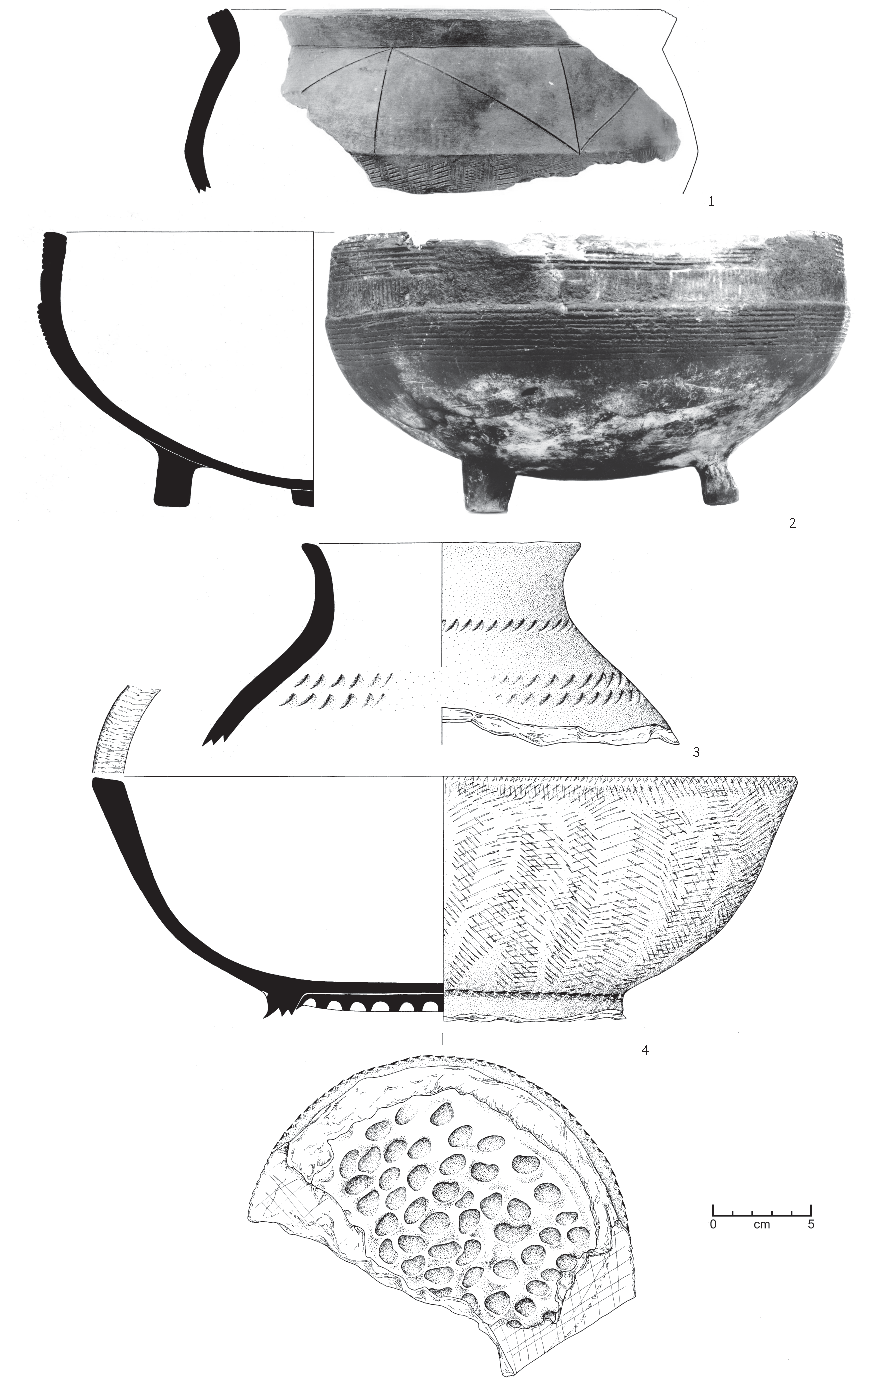
\includegraphics{plt/Taf1.pdf}
	\vspace{.75em}\caption{\mbox{Ubangi}, Oberflächenfunde \\ 1 BRU~85/101; 2 LKK~85/101; 3--4 BOB~85/101.}
	\label{pl:1}
\end{pl}

\begin{pl}[H]
	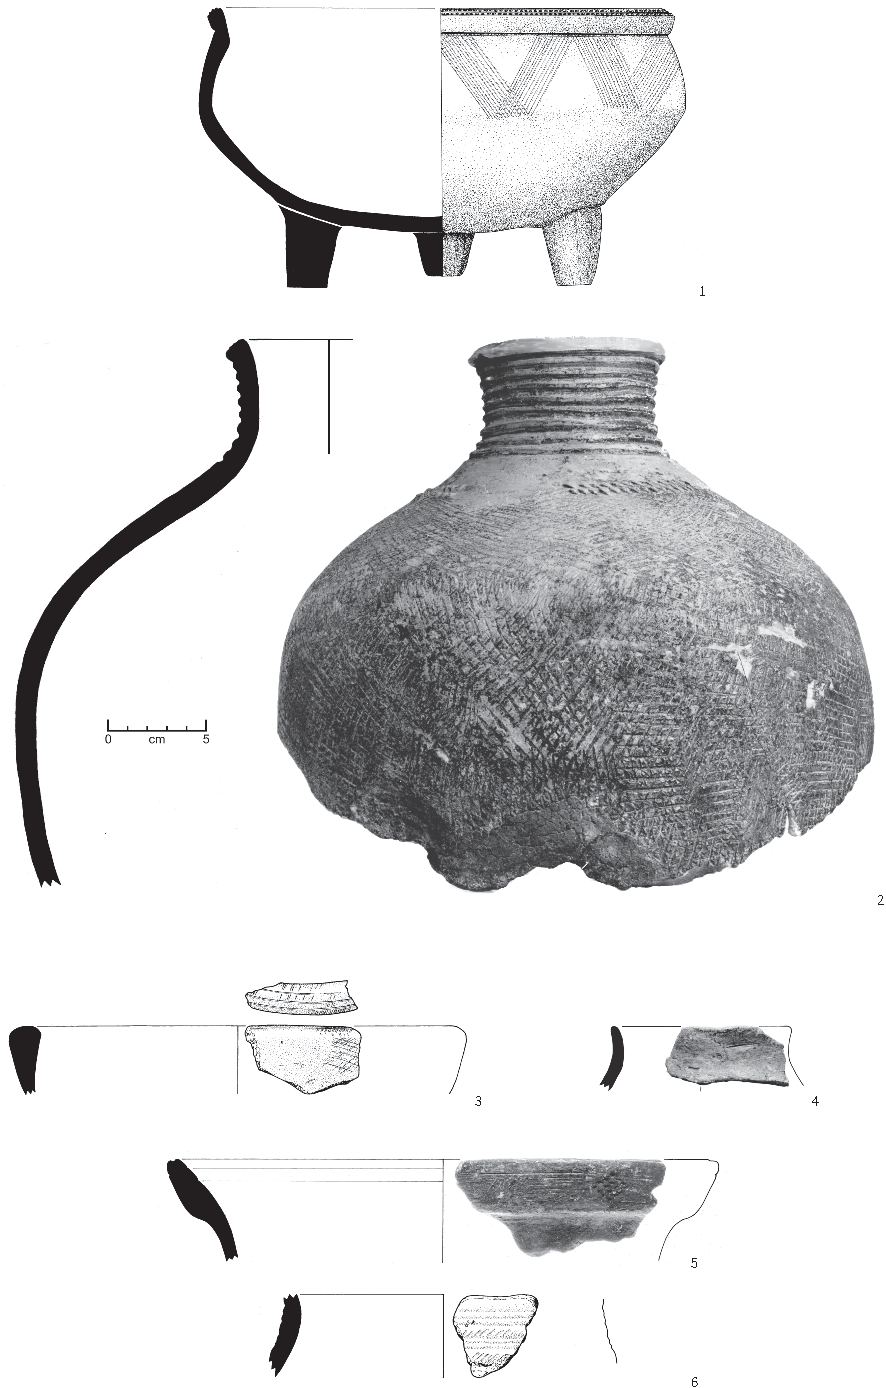
\includegraphics{plt/Taf2.pdf}
	\vspace{.75em}\caption{\mbox{Ubangi}, Oberflächenfunde \\ 1--2 BWK~85/101; 3--7 ZAM~85/101.}
	\label{pl:2}
\end{pl}

\begin{pl}[H]
	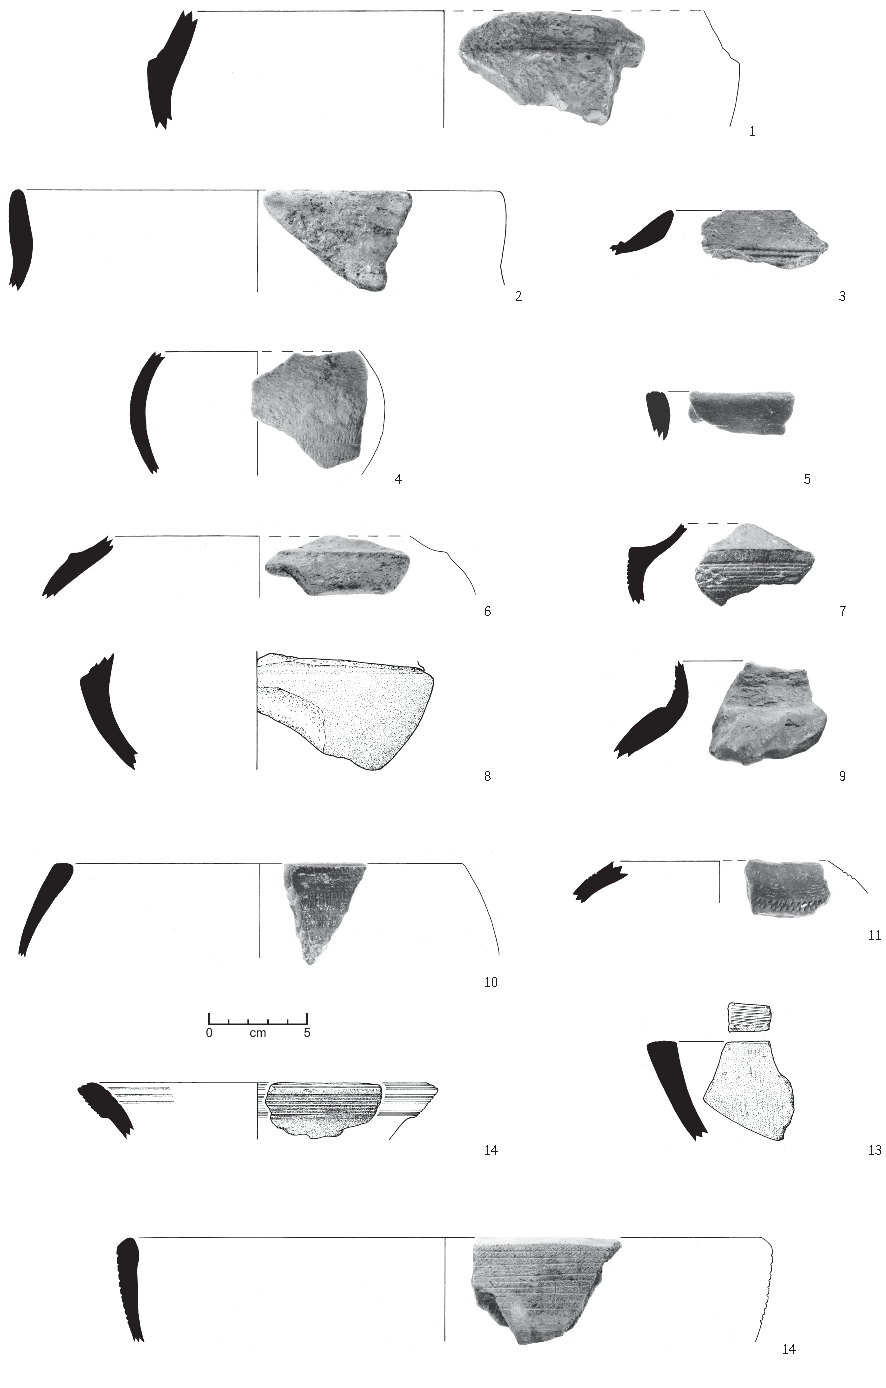
\includegraphics{plt/Taf3.pdf}
	\vspace{.75em}\caption{\mbox{Ubangi}, Oberflächenfunde \\ 1--11 ZAM~85/101; 12--13 ILA~85/101; 14--15 LKA~85/101.}
	\label{pl:3}
\end{pl}

\begin{pl}[H]
	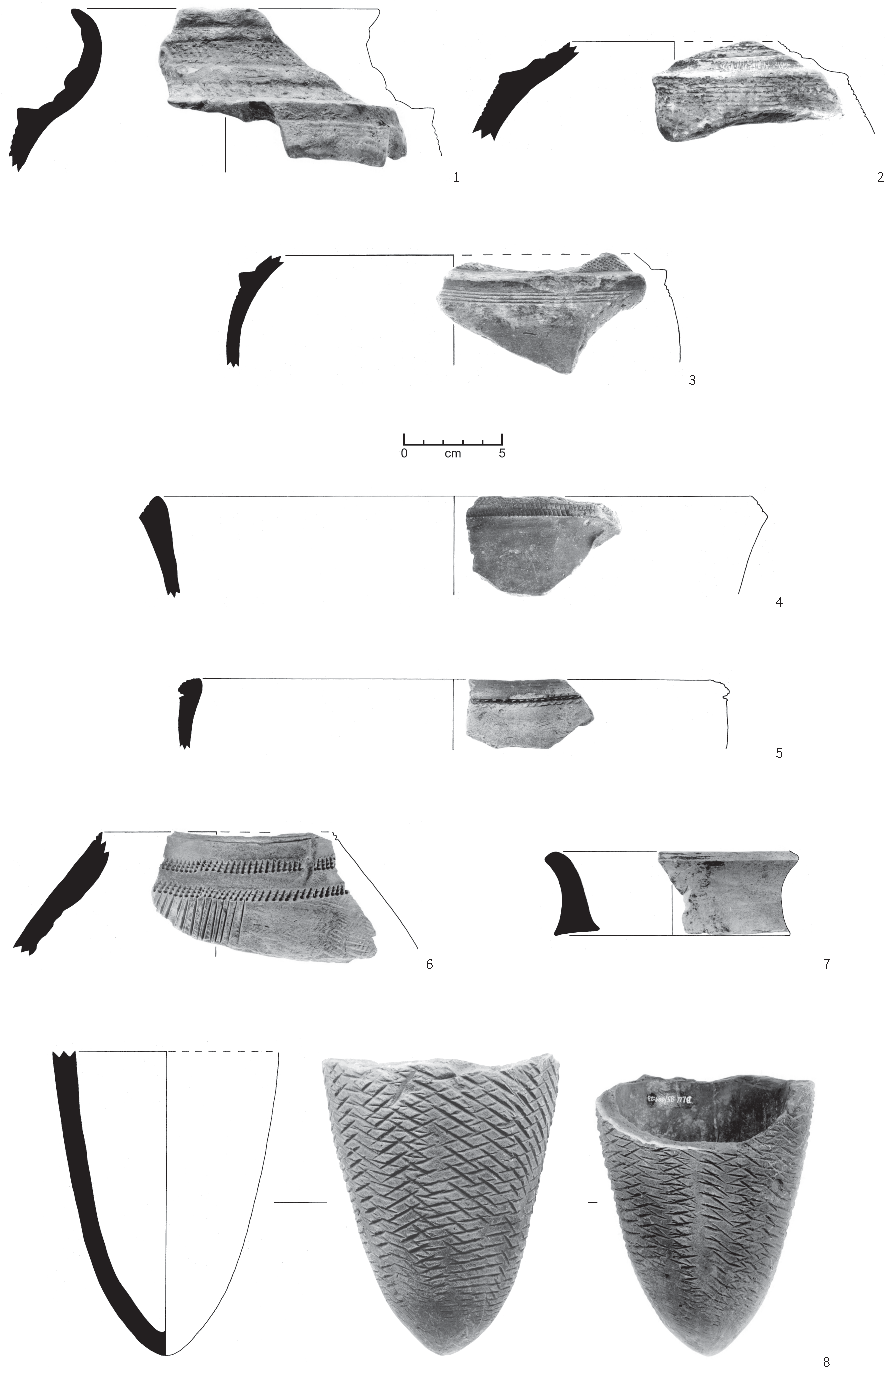
\includegraphics{plt/Taf4.pdf}
	\vspace{.75em}\caption{\mbox{Ubangi}, Oberflächenfunde \\ 1--3 LKA~85/101; 4--8 BLU~85/101.}
	\label{pl:4}
\end{pl}

\begin{pl}[H]
	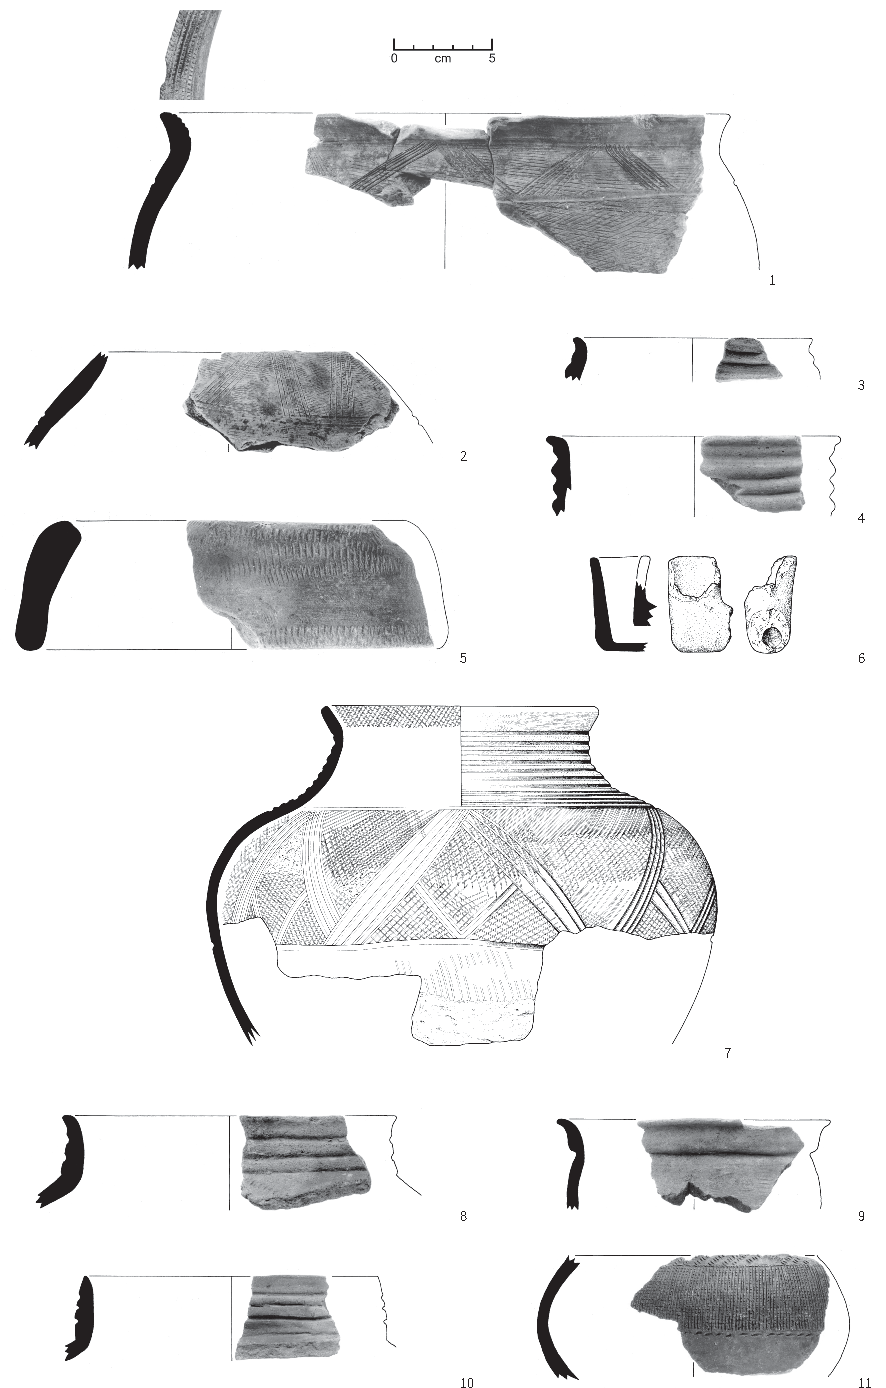
\includegraphics{plt/Taf5.pdf}
	\vspace{.75em}\caption{\mbox{Ubangi}, Oberflächenfunde \\ 1--6 BYO~85/101; 7 EBE~85/101; 8--11 BBL~85/101.}
	\label{pl:5}
\end{pl}

\begin{pl}[H]
	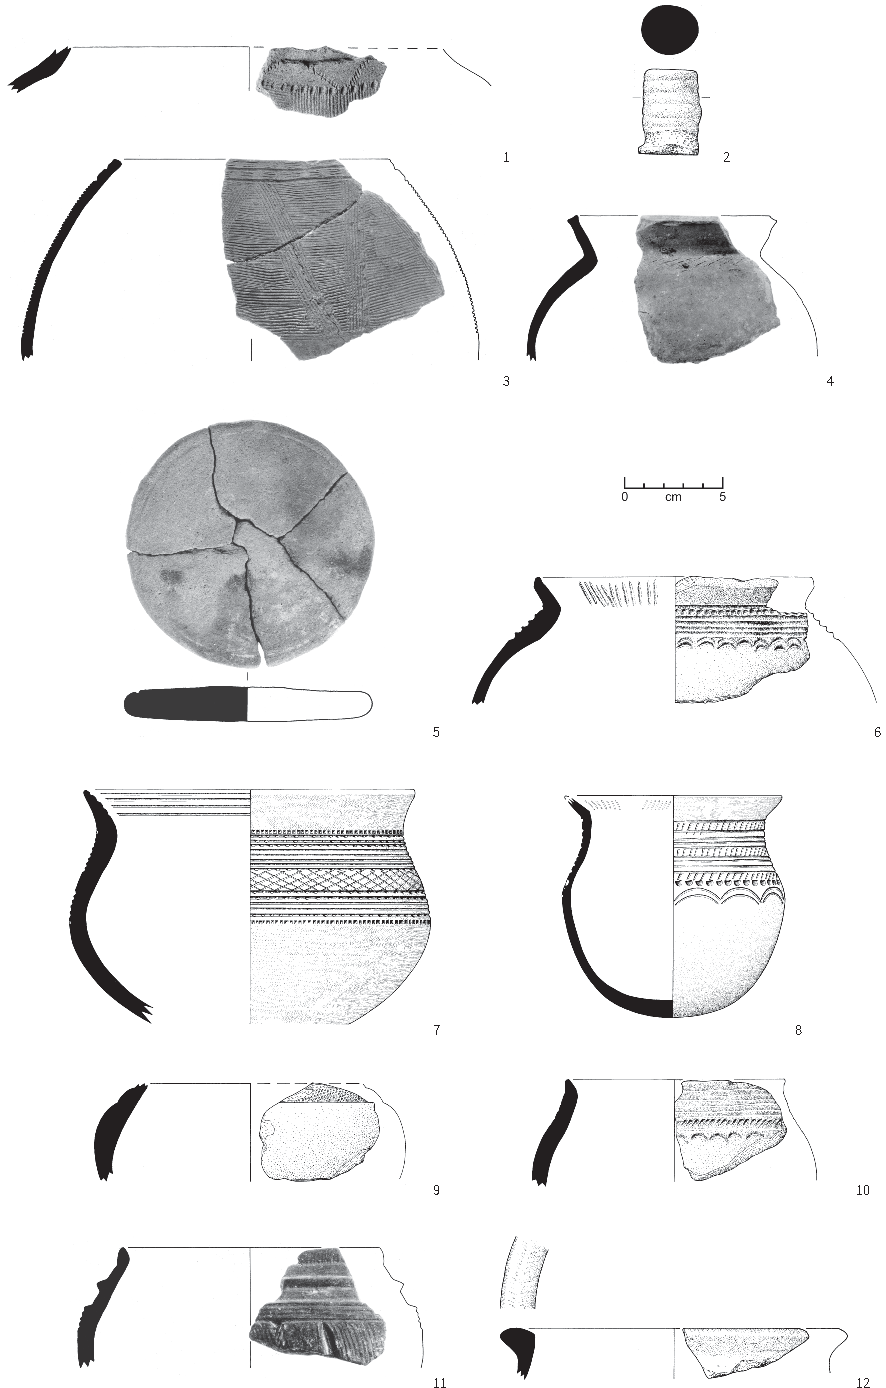
\includegraphics{plt/Taf6.pdf}
	\vspace{.75em}\caption{\mbox{Ubangi}, Oberflächenfunde \\ 1--2 BBL~85/101; 3--5 BBL~85/102; 6--12 NGB~85/101.}
	\label{pl:6}
\end{pl}

\begin{pl}[H]
	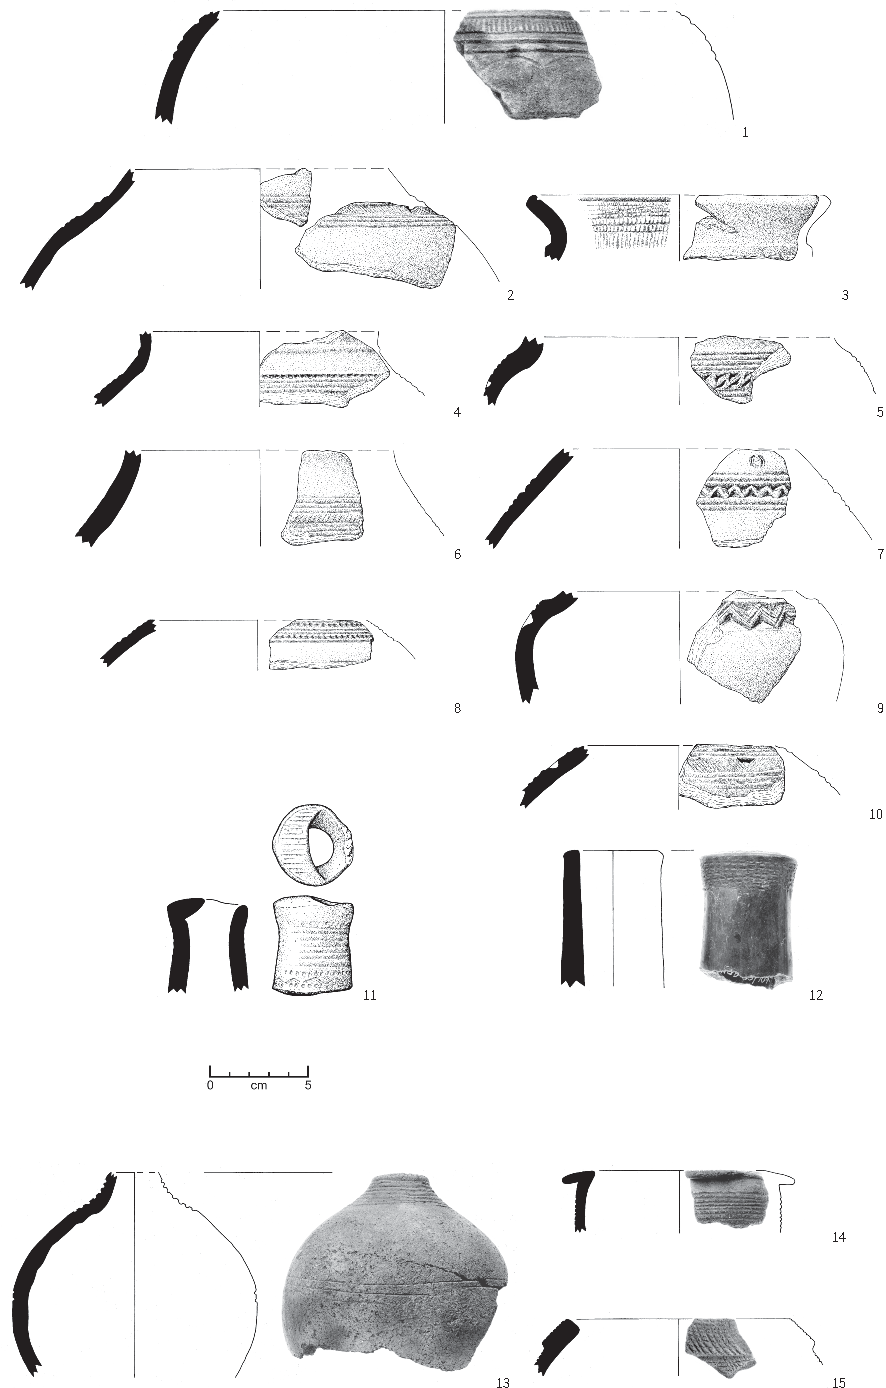
\includegraphics{plt/Taf7.pdf}
	\vspace{.75em}\caption{\mbox{Ubangi}, Oberflächenfunde \\ 1--12 NGB~85/101; 13 BMN~85/101; 14--16 DON~85/101.}
	\label{pl:7}
\end{pl}

\begin{pl}[H]
	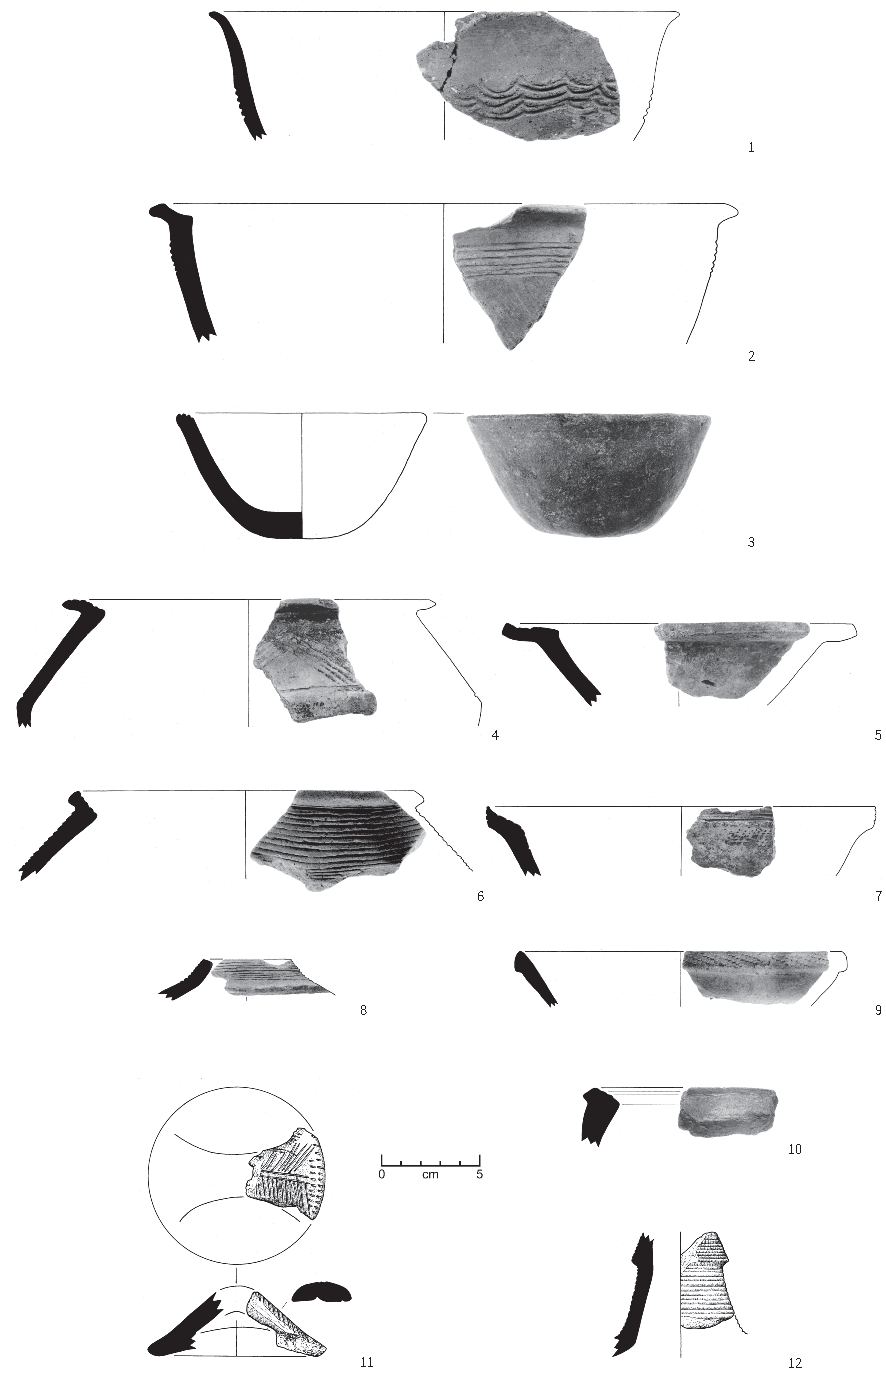
\includegraphics{plt/Taf8.pdf}
	\vspace{.75em}\caption{\mbox{Ubangi}, Oberflächenfunde \\ 1--12 DON~85/101.}
	\label{pl:8}
\end{pl}

\begin{pl}[H]
	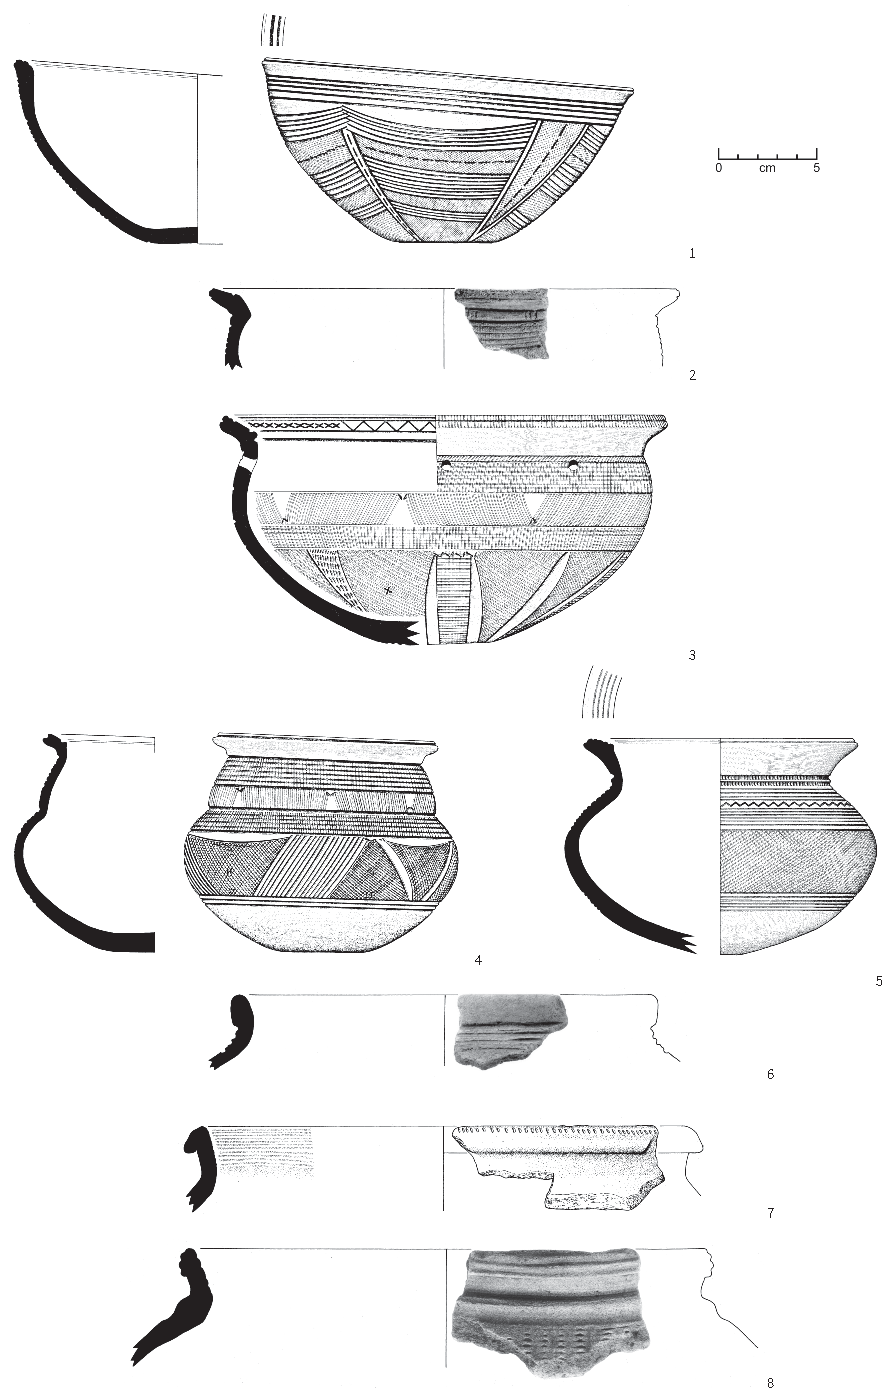
\includegraphics{plt/Taf9.pdf}
	\vspace{.75em}\caption{\mbox{Ubangi}, Oberflächenfunde \\ 1--6 DON~85/102; 7--8 MBN~85/101.}
	\label{pl:9}
\end{pl}

\begin{pl}[H]
	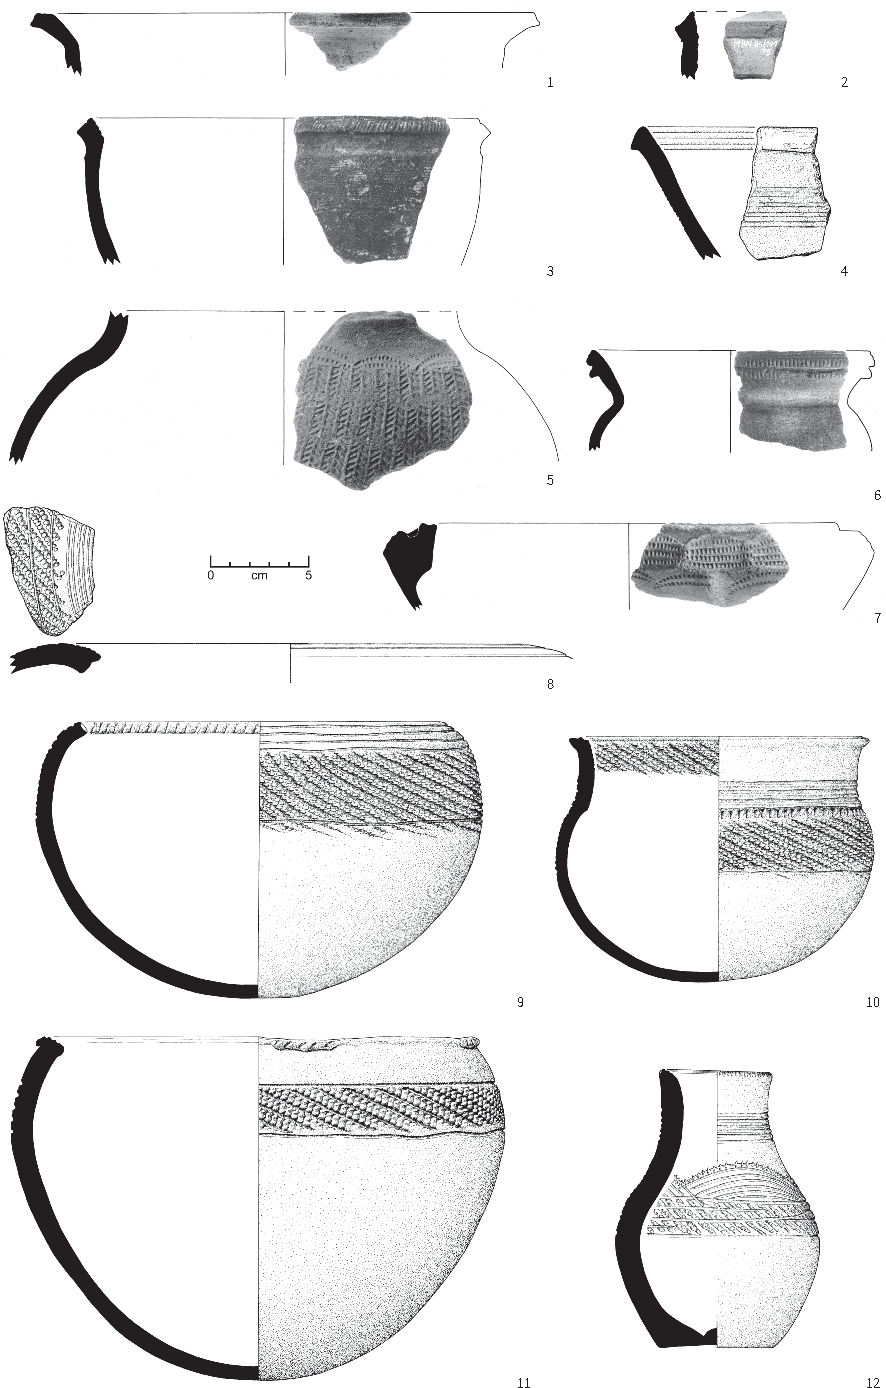
\includegraphics{plt/Taf10.pdf}
	\vspace{.75em}\caption{\mbox{Ubangi}, Oberflächenfunde \& Ankauf (9--12) \\ 1--8 MBN~85/101; 9--11 MBN~85/501; 12 MBN~85/502.}
	\label{pl:10}
\end{pl}

\begin{pl}[H]
	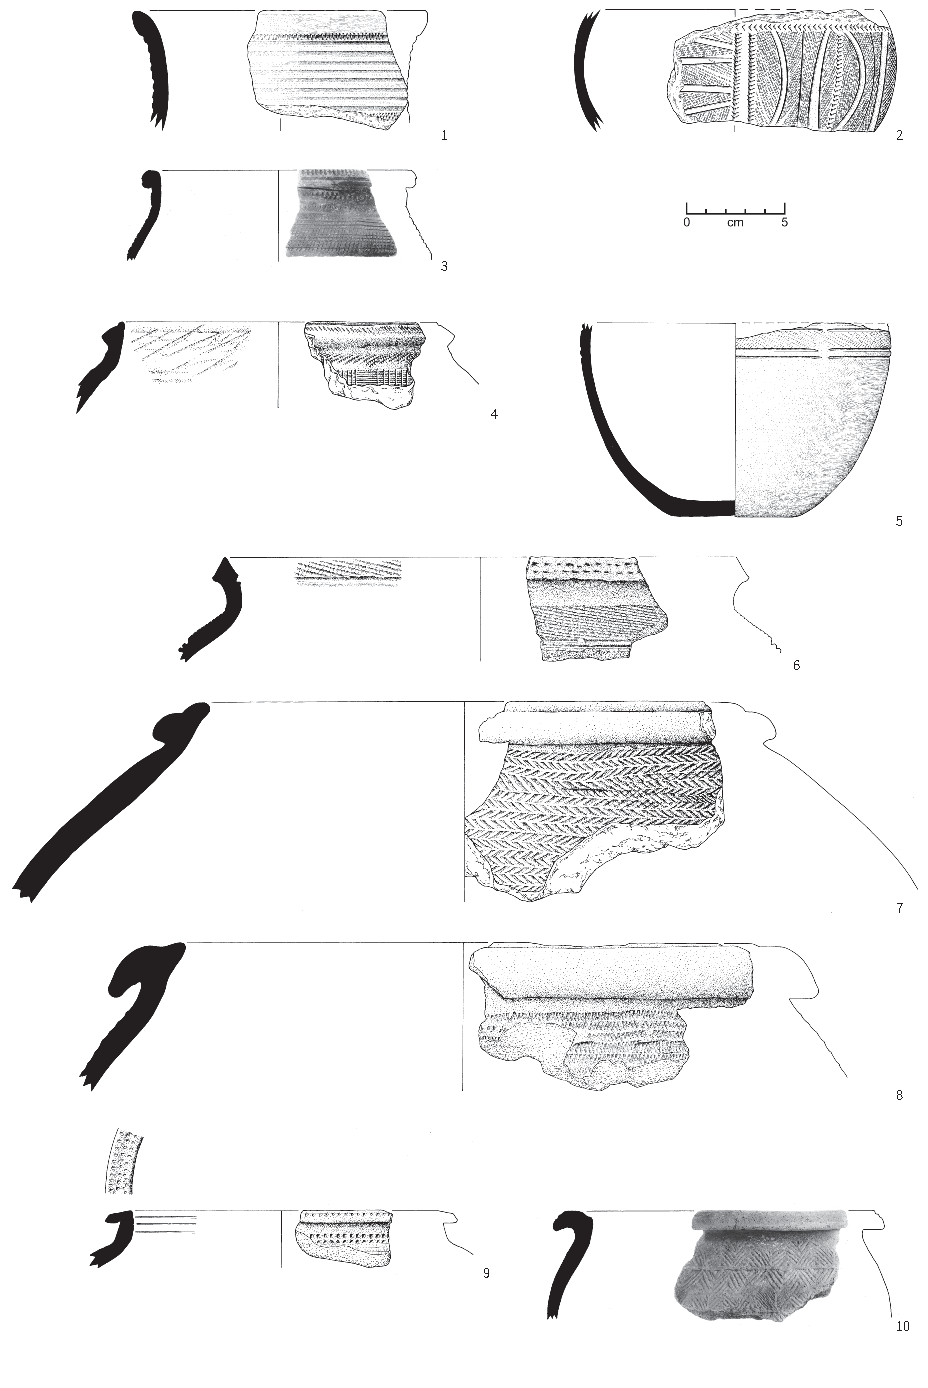
\includegraphics{plt/Taf11.pdf}
	\vspace{.75em}\caption{\mbox{Ubangi}, Oberflächenfunde \\ 1--3 NZA~85/101; 4--10 MTB~85/101.}
	\label{pl:11}
\end{pl}

\begin{pl}[H]
	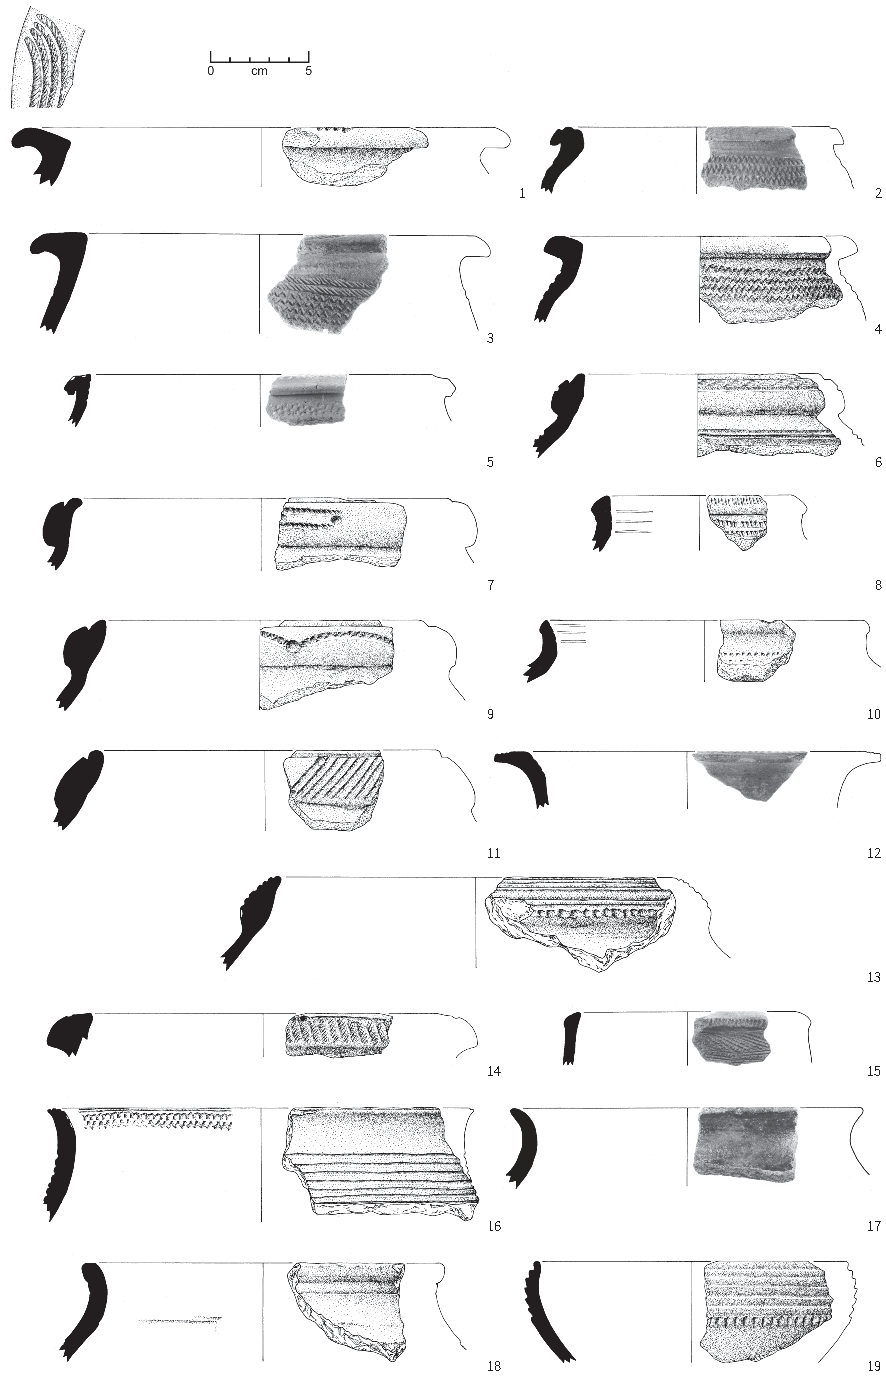
\includegraphics{plt/Taf12.pdf}
	\vspace{.75em}\caption{\mbox{Ubangi}, Oberflächenfunde \\ 1--20 MTB~85/101.}
	\label{pl:12}
\end{pl}

\begin{pl}[H]
	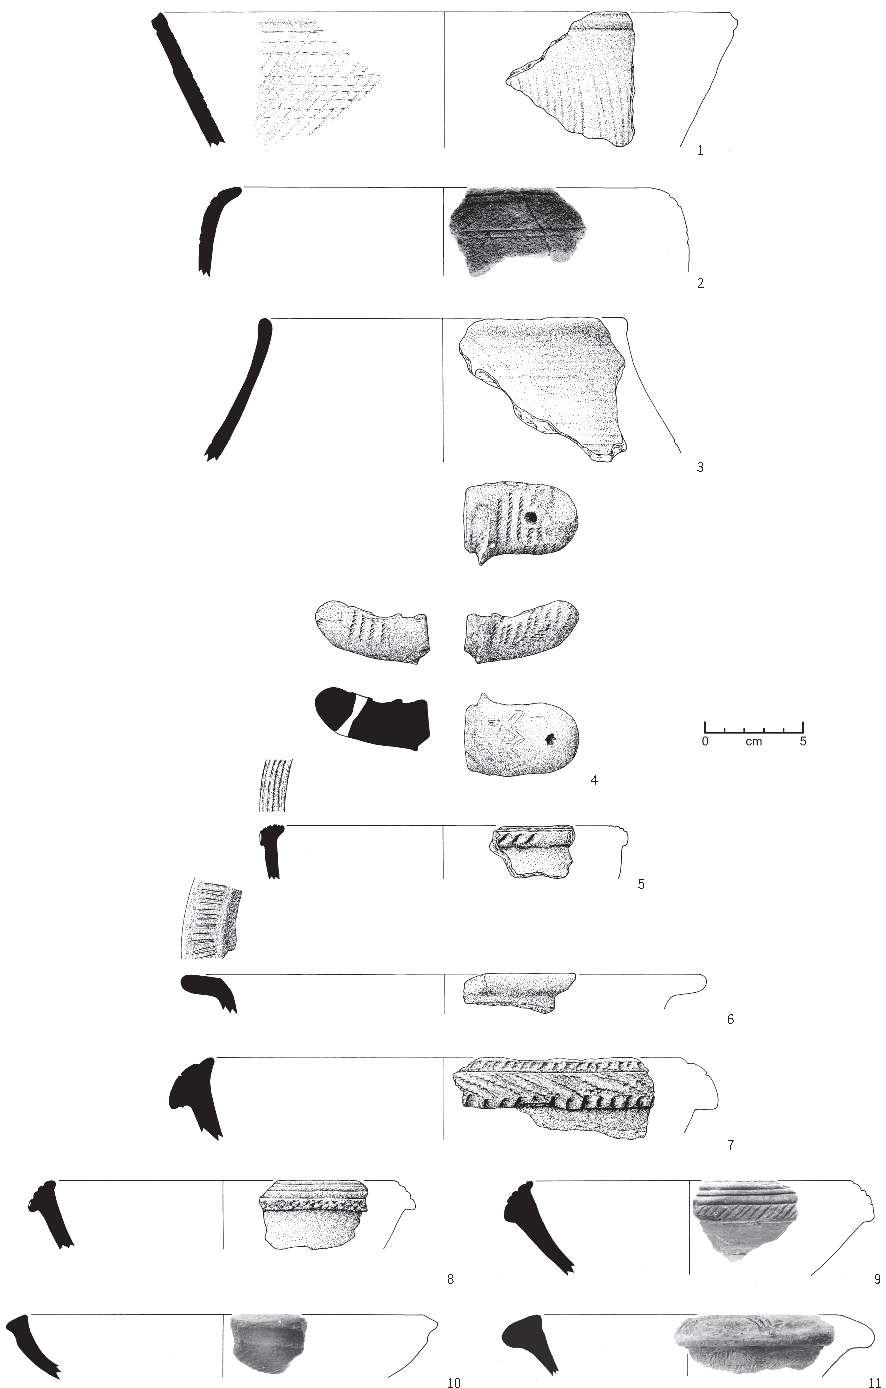
\includegraphics{plt/Taf13.pdf}
	\vspace{.75em}\caption{\mbox{Ubangi}, Oberflächenfunde \\ 1--11 MTB~85/101.}
	\label{pl:13}
\end{pl}

\begin{pl}[H]
	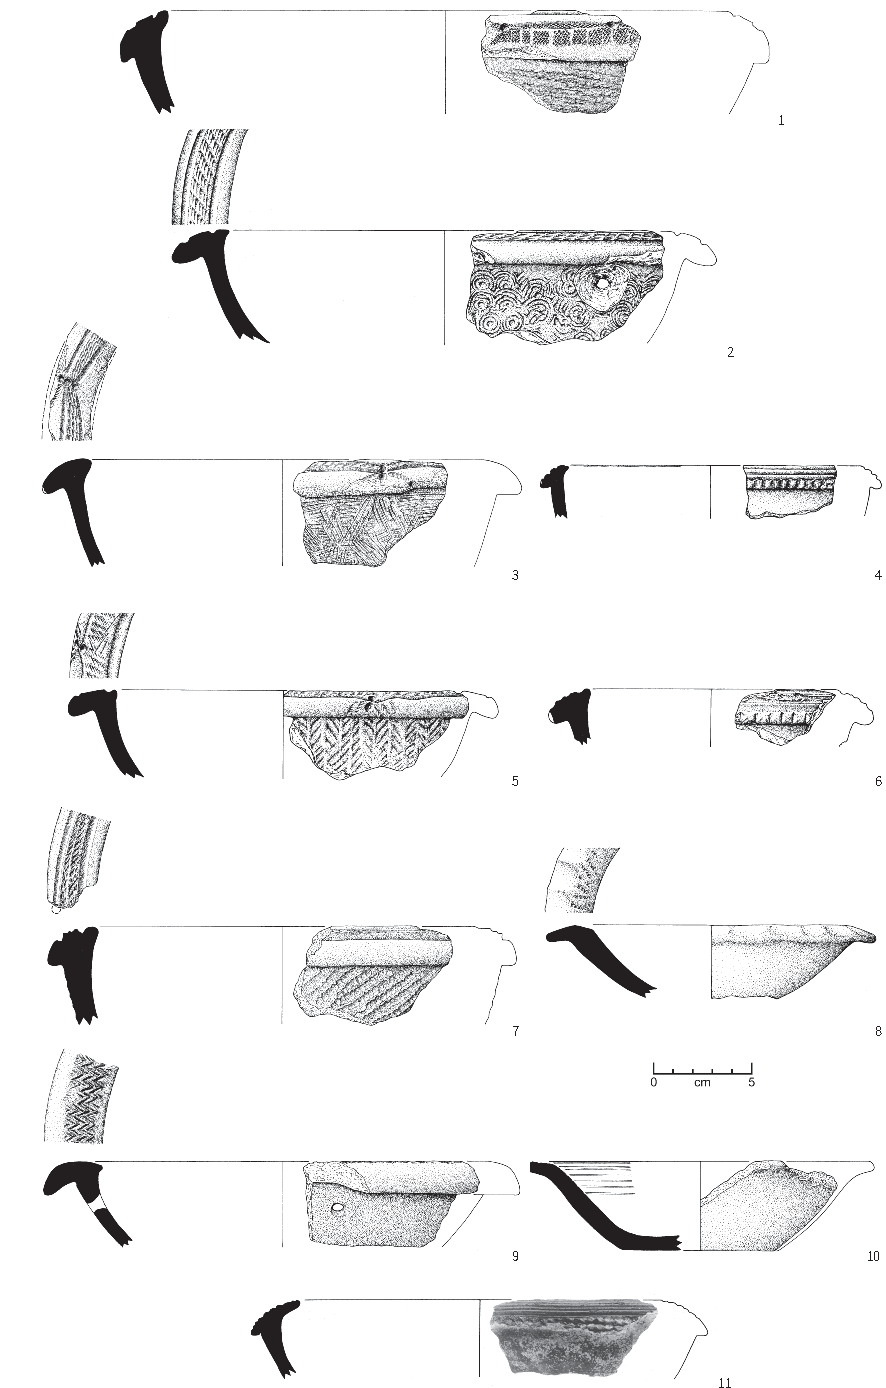
\includegraphics{plt/Taf14.pdf}
	\vspace{.75em}\caption{\mbox{Ubangi}, Oberflächenfunde \\ 1--11 MTB~85/101.}
	\label{pl:14}
\end{pl}

\begin{pl}[H]
	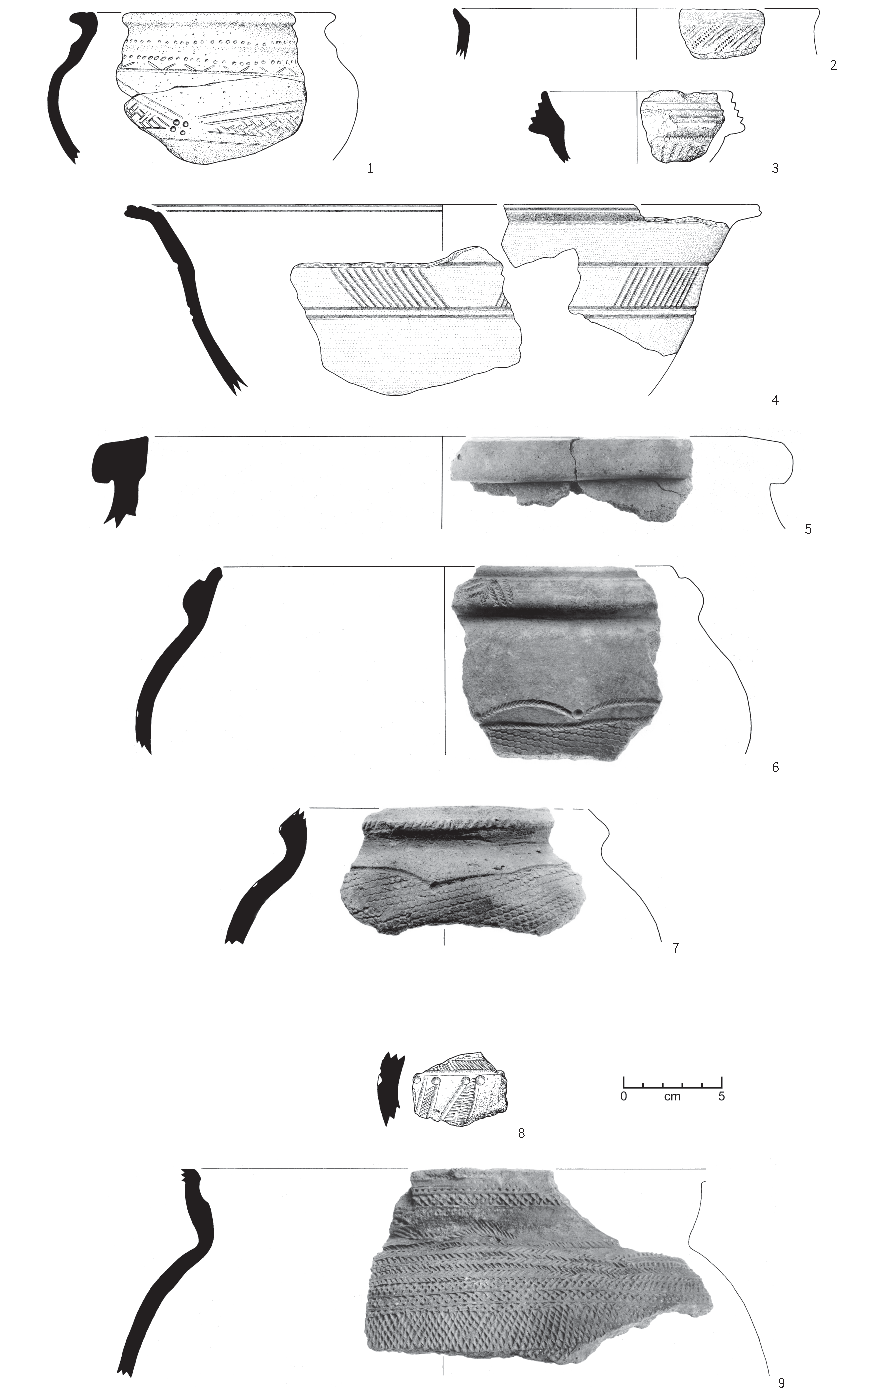
\includegraphics{plt/Taf15.pdf}
	\vspace{.75em}\caption{\mbox{Ubangi}, Oberflächenfunde \\ 1--7 MAO~85/101; 8--9 LIB~85/101.}
	\label{pl:15}
\end{pl}

\begin{pl}[H]
	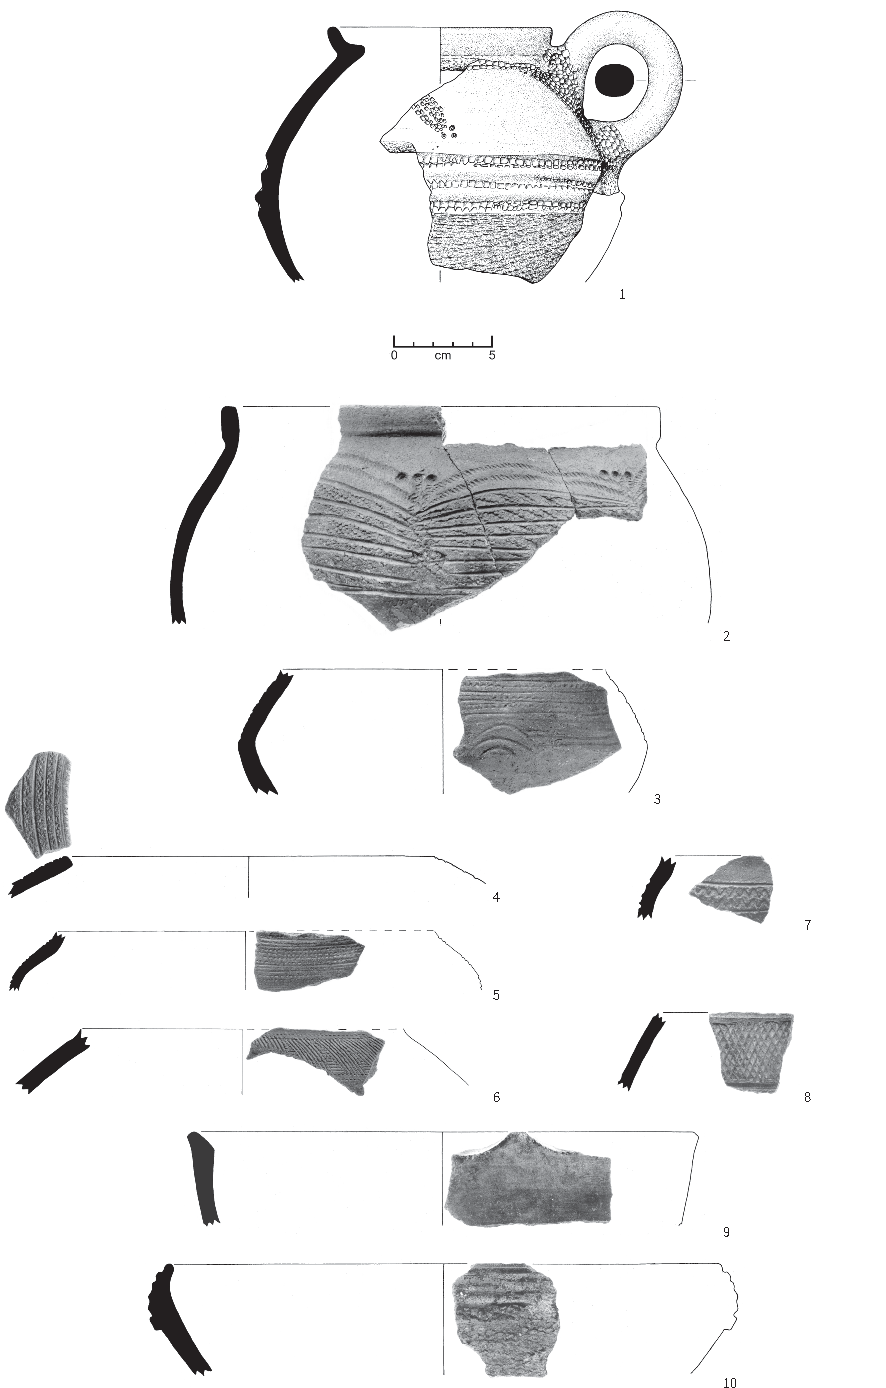
\includegraphics{plt/Taf16.pdf}
	\vspace{.75em}\caption{\mbox{Ubangi}, Oberflächenfunde \\ 1 LIB~85/101; 2--10 BAT~85/101}
	\label{pl:16}
\end{pl}

\begin{pl}[H]
	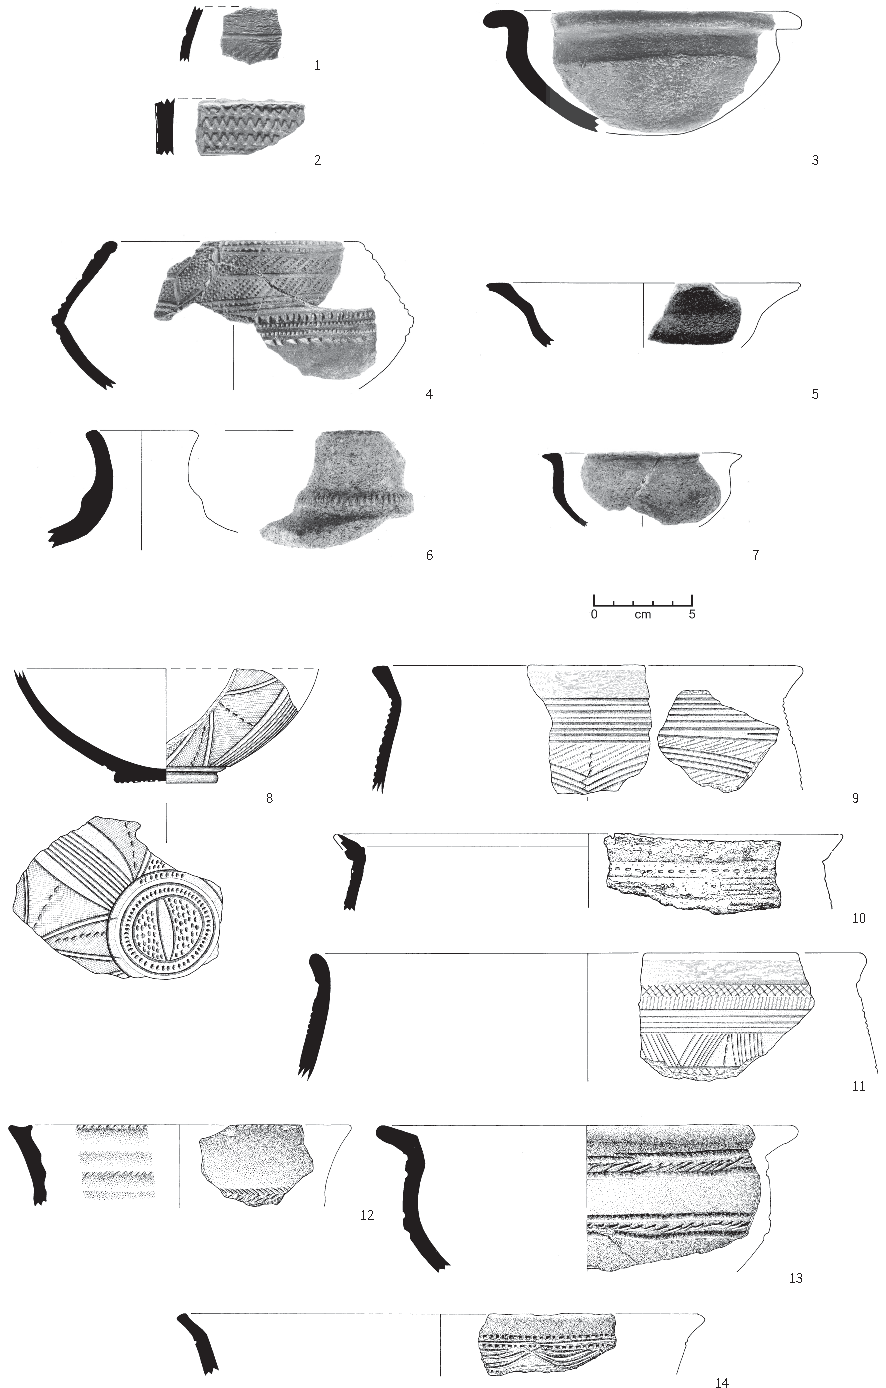
\includegraphics{plt/Taf17.pdf}
	\vspace{.75em}\caption{\mbox{Ubangi}, Oberflächenfunde \\ 1--2 BMK~85/101; 3 MBO~85/101; 4--7 MND~85/101; 8--14 MKL~85/101.}
	\label{pl:17}
\end{pl}


\begin{pl}[H]
	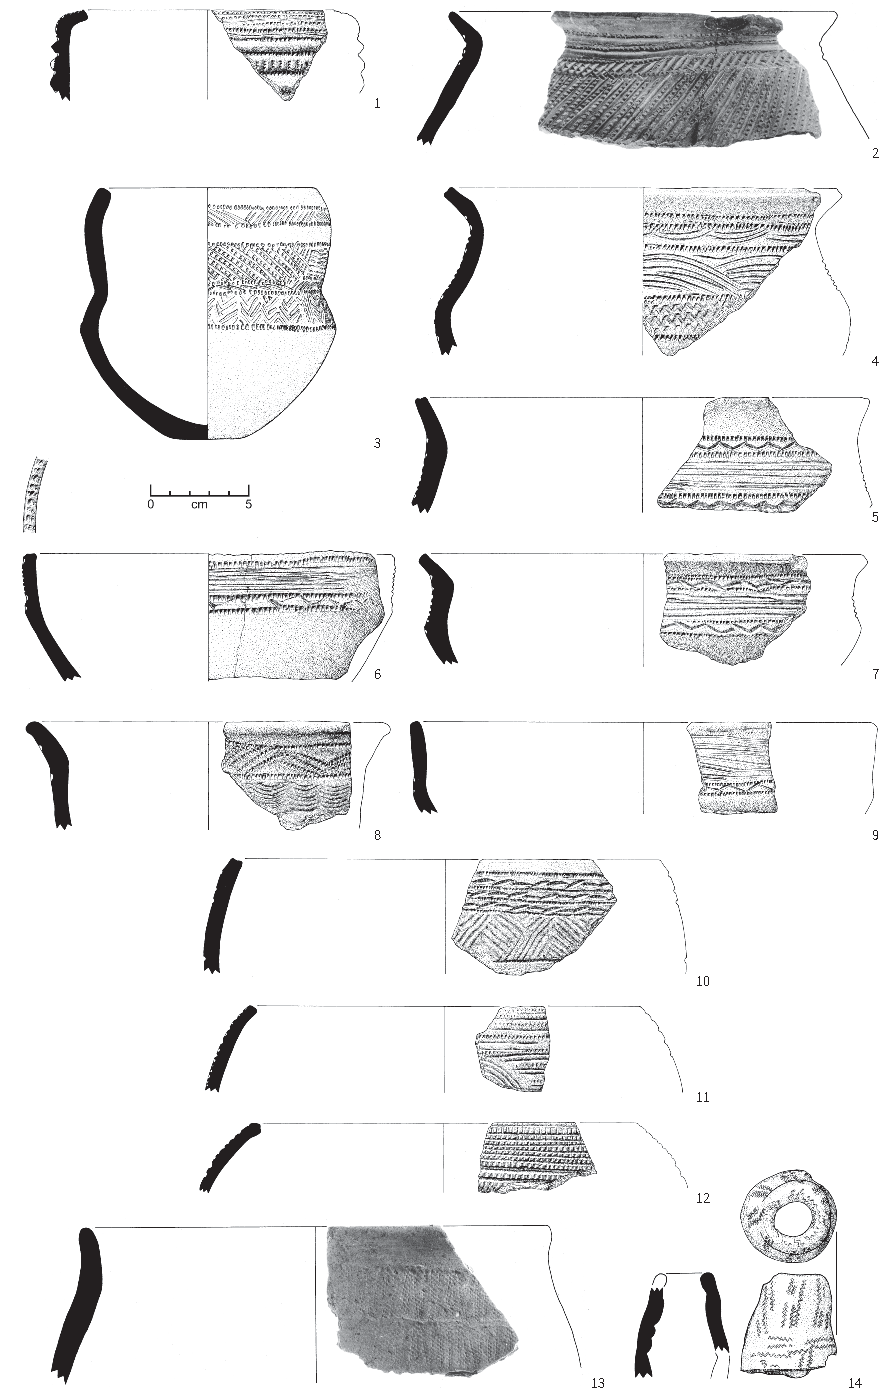
\includegraphics{plt/Taf18.pdf}
	\vspace{.75em}\caption{\mbox{Ubangi}, Oberflächenfunde \\ 1--14 MKL~85/101.}
	\label{pl:18}
\end{pl}

\begin{pl}[H]
	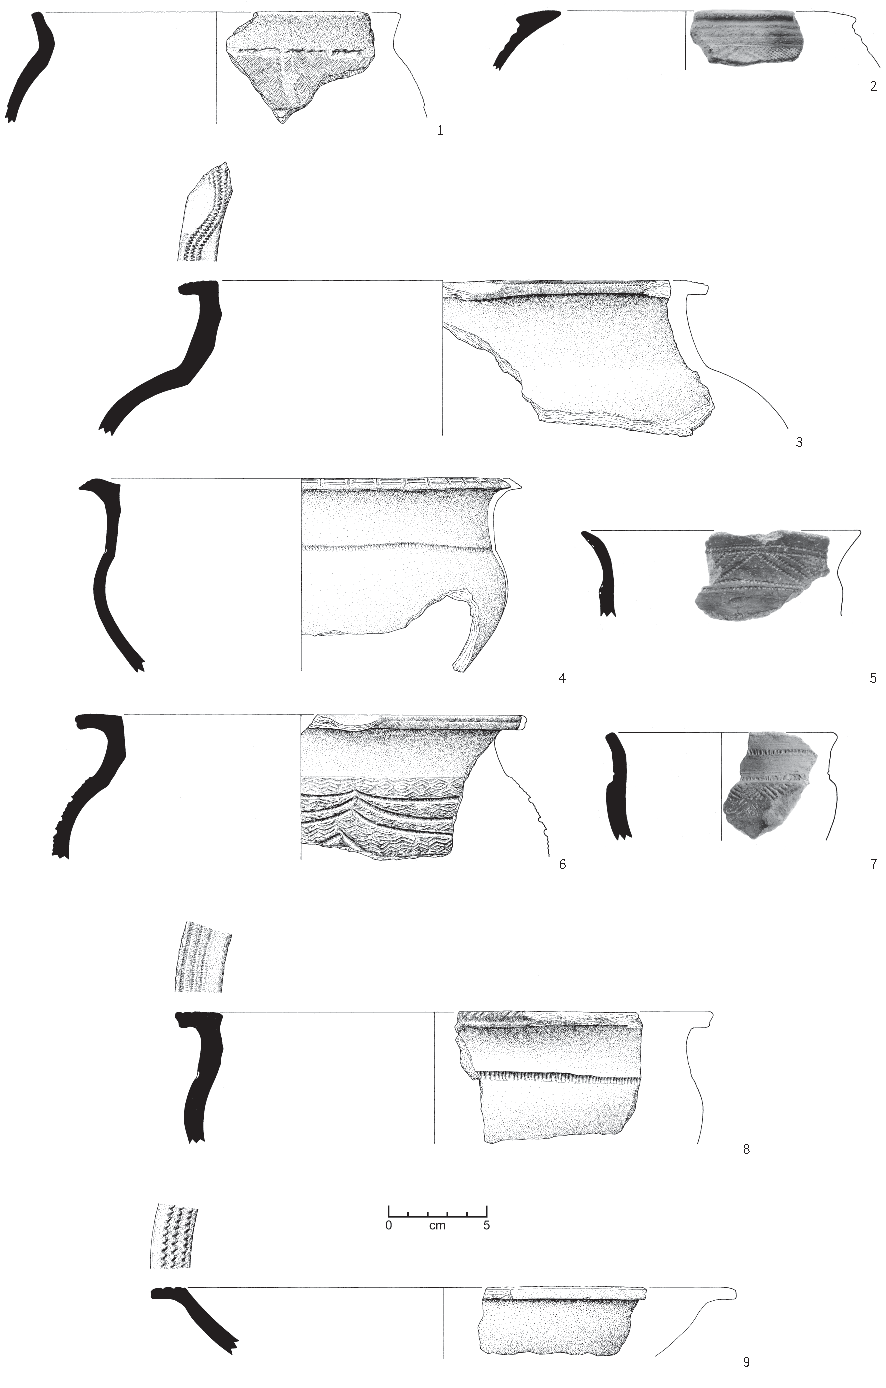
\includegraphics{plt/Taf19.pdf}
	\vspace{.75em}\caption{\mbox{Ubangi}, Oberflächenfunde \\ 1--9 MKL~85/101.}
	\label{pl:19}
\end{pl}

\begin{pl}[H]
	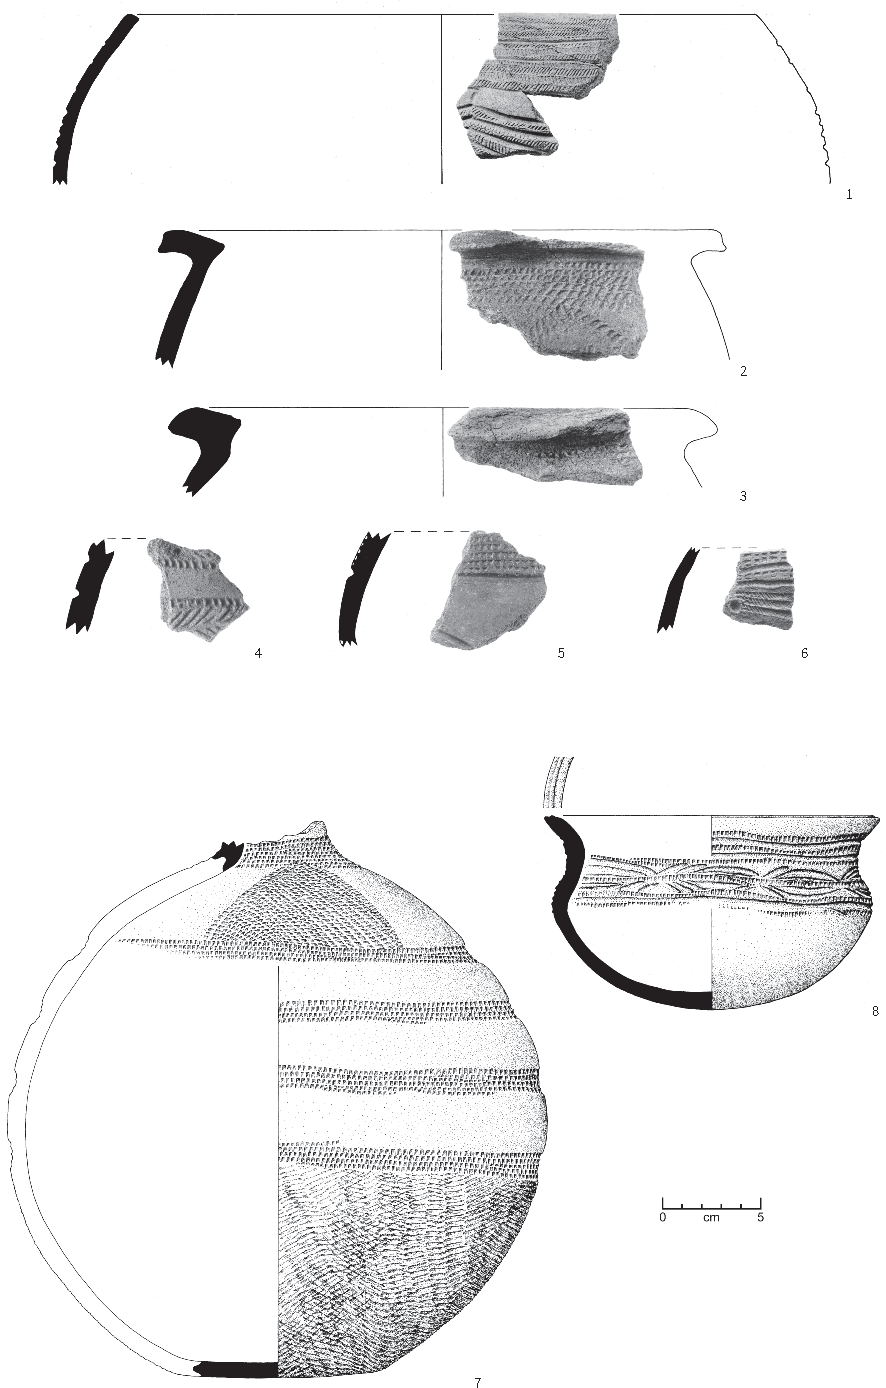
\includegraphics{plt/Taf20.pdf}
	\vspace{.75em}\caption{\mbox{Ubangi}, Oberflächenfunde \\ 1--6 BLN~85/101; 7--8 BLN~85/201.}
	\label{pl:20}
\end{pl}

\begin{pl}[H]
	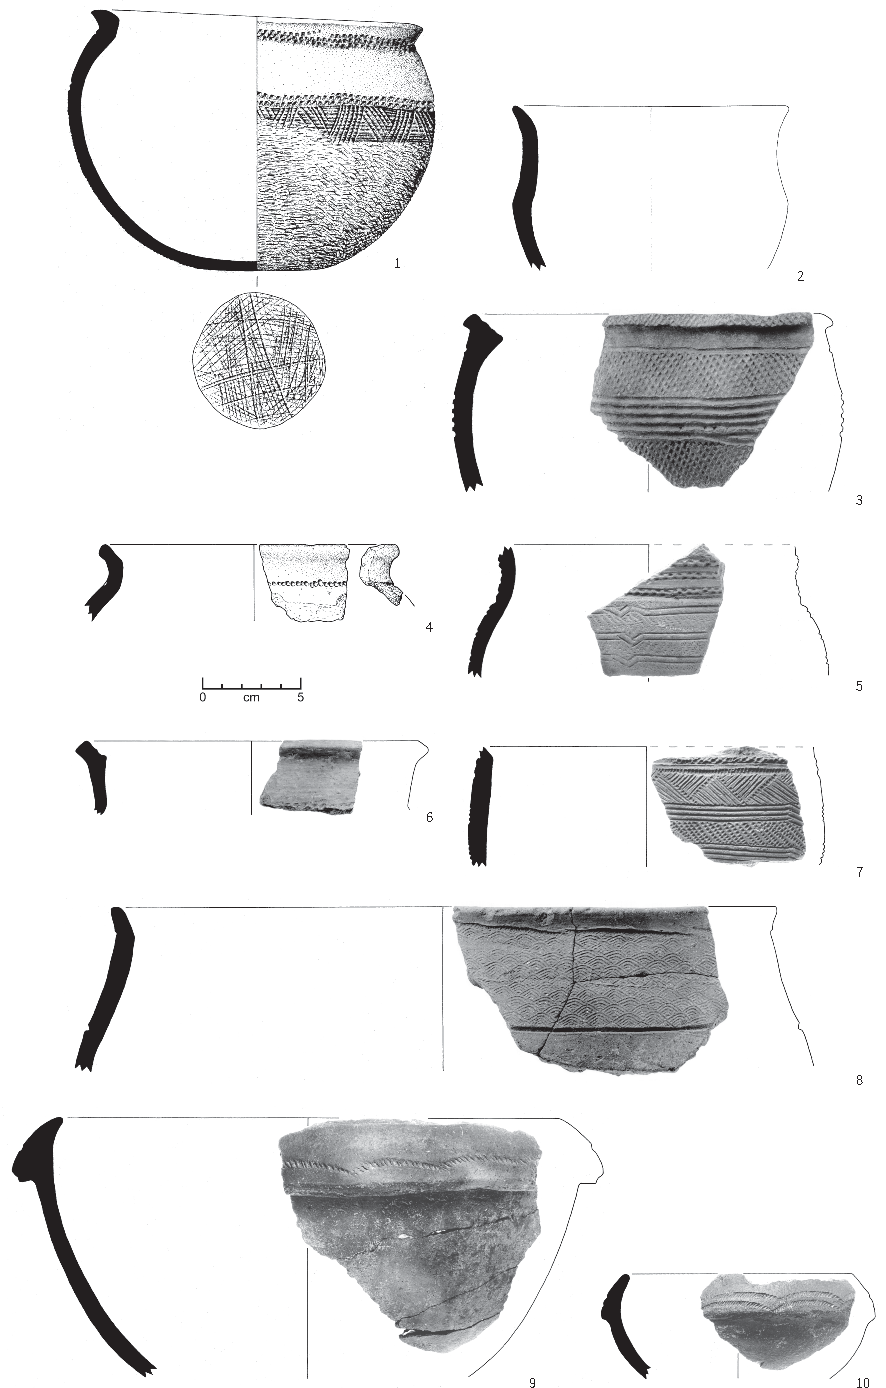
\includegraphics{plt/Taf21.pdf}
	\vspace{.75em}\caption{\mbox{Ubangi}, Oberflächenfunde \\ 1 BAN~85/101; 2--11 MBK~85/101.}
	\label{pl:21}
\end{pl}

\begin{pl}[H]
	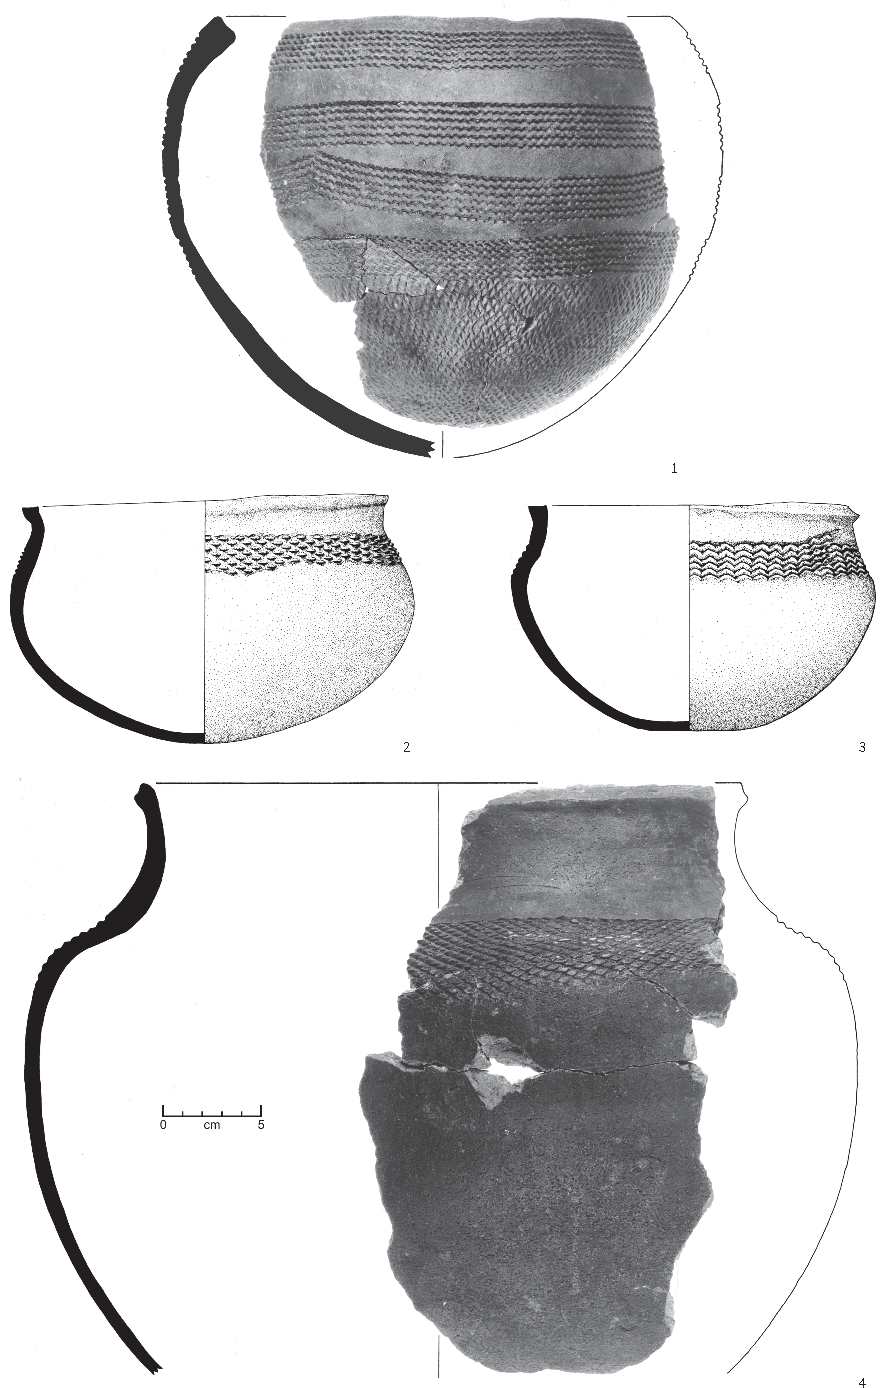
\includegraphics{plt/Taf22.pdf}
	\vspace{.75em}\caption{\mbox{Ubangi}, Oberflächenfunde \& Ankauf (2--3) \\ 1 KPT~85/101; 2--3 DAM~85/503; 4 DOK~85/101.}
	\label{pl:22}
\end{pl}

\begin{pl}[H]
	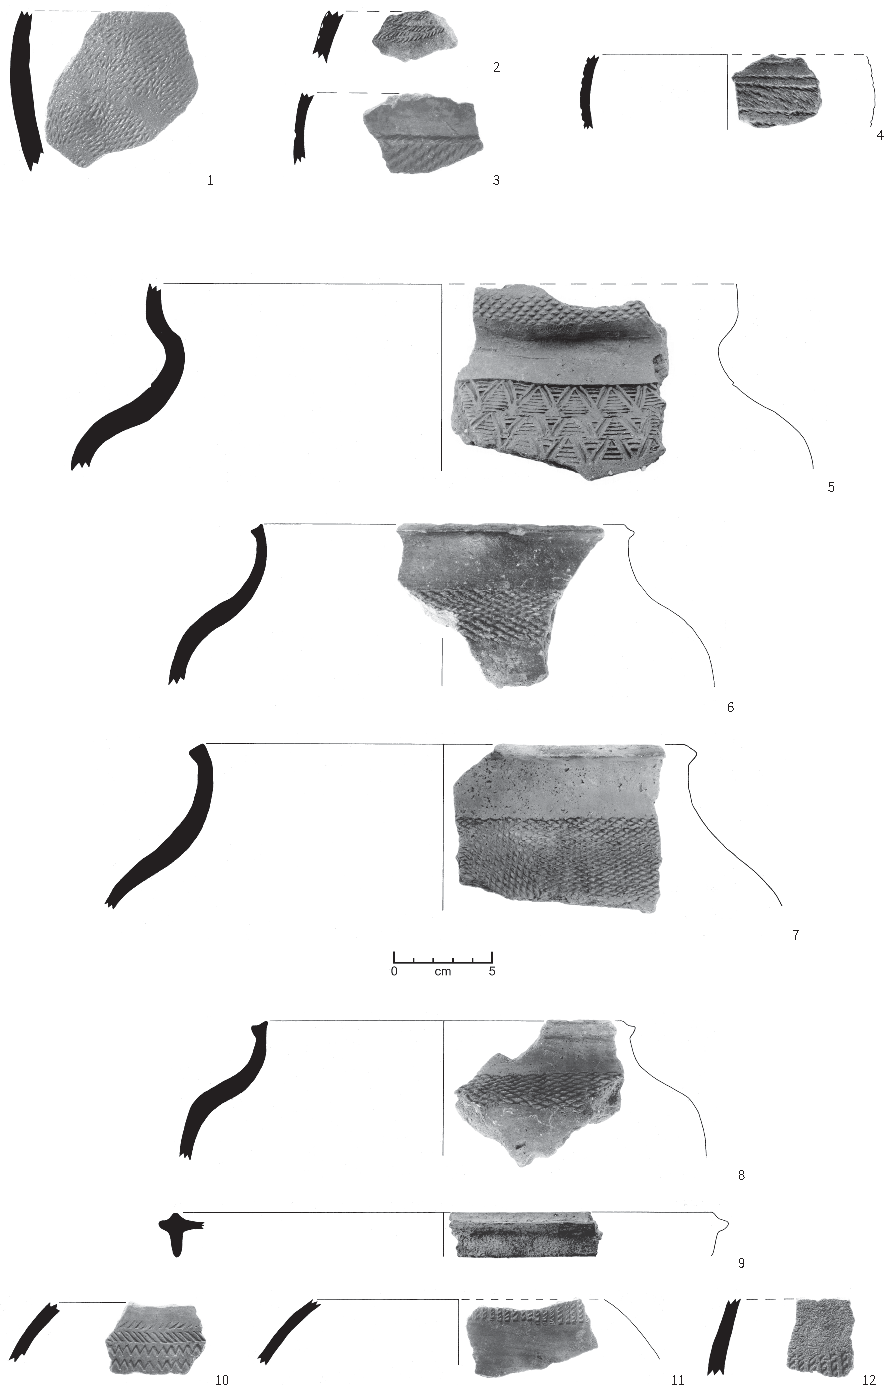
\includegraphics{plt/Taf23.pdf}
	\vspace{.75em}\caption{\mbox{Ubangi}, Oberflächenfunde \\ 1--4 DOK~85/101; 5--7 BOD~85/101; 8--12 GBA~85/101.}
	\label{pl:23}
\end{pl}

\begin{pl}[H]
	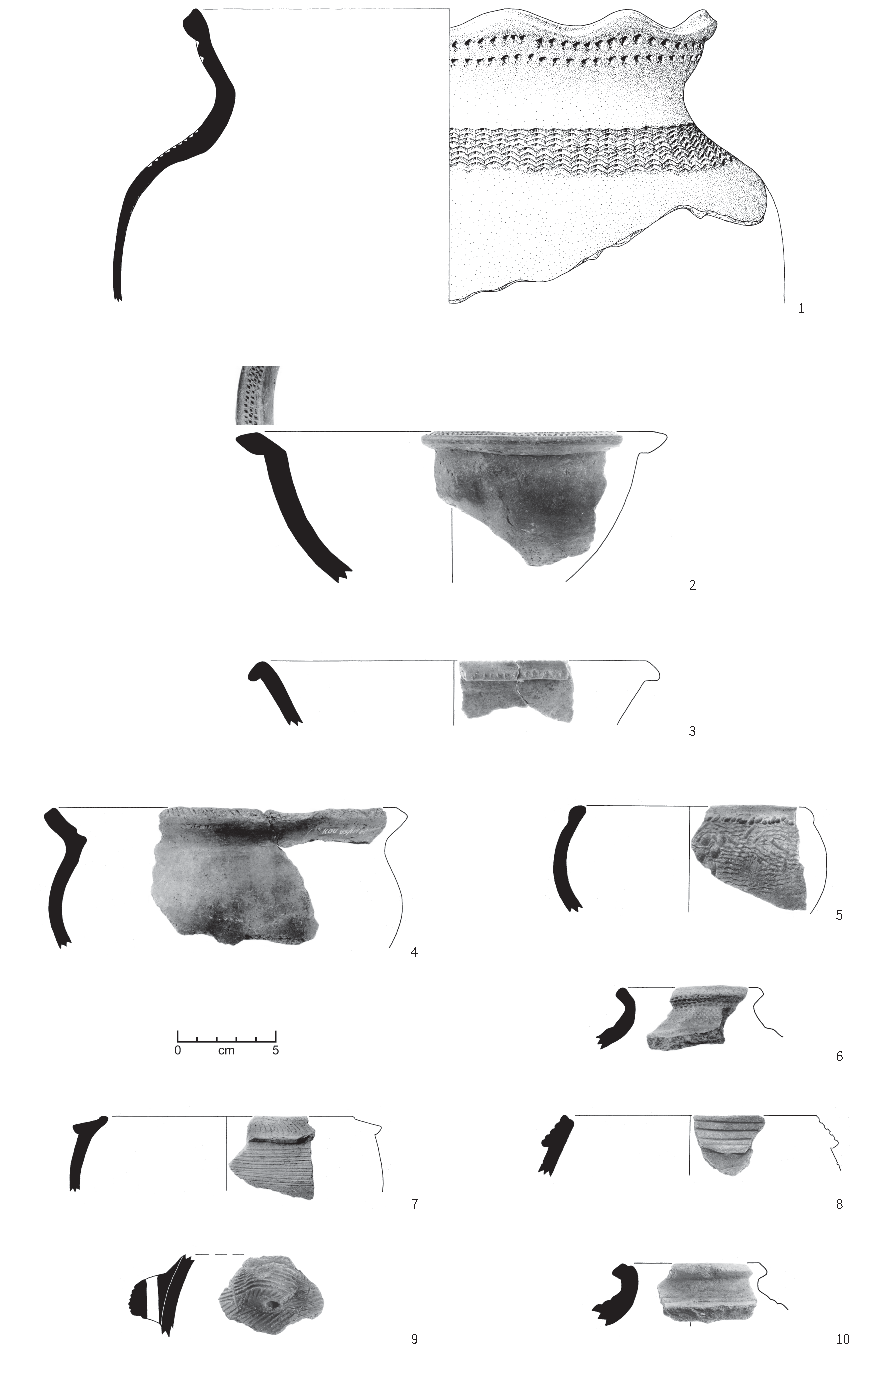
\includegraphics{plt/Taf24.pdf}
	\vspace{.75em}\caption{\mbox{Ubangi} \& Lua, Oberflächenfunde \\ 1 NDG~85/101; 2--7 KOU~85/101; 8--14 MLB~85/101.}
	\label{pl:24}
\end{pl}

\begin{pl}[H]
	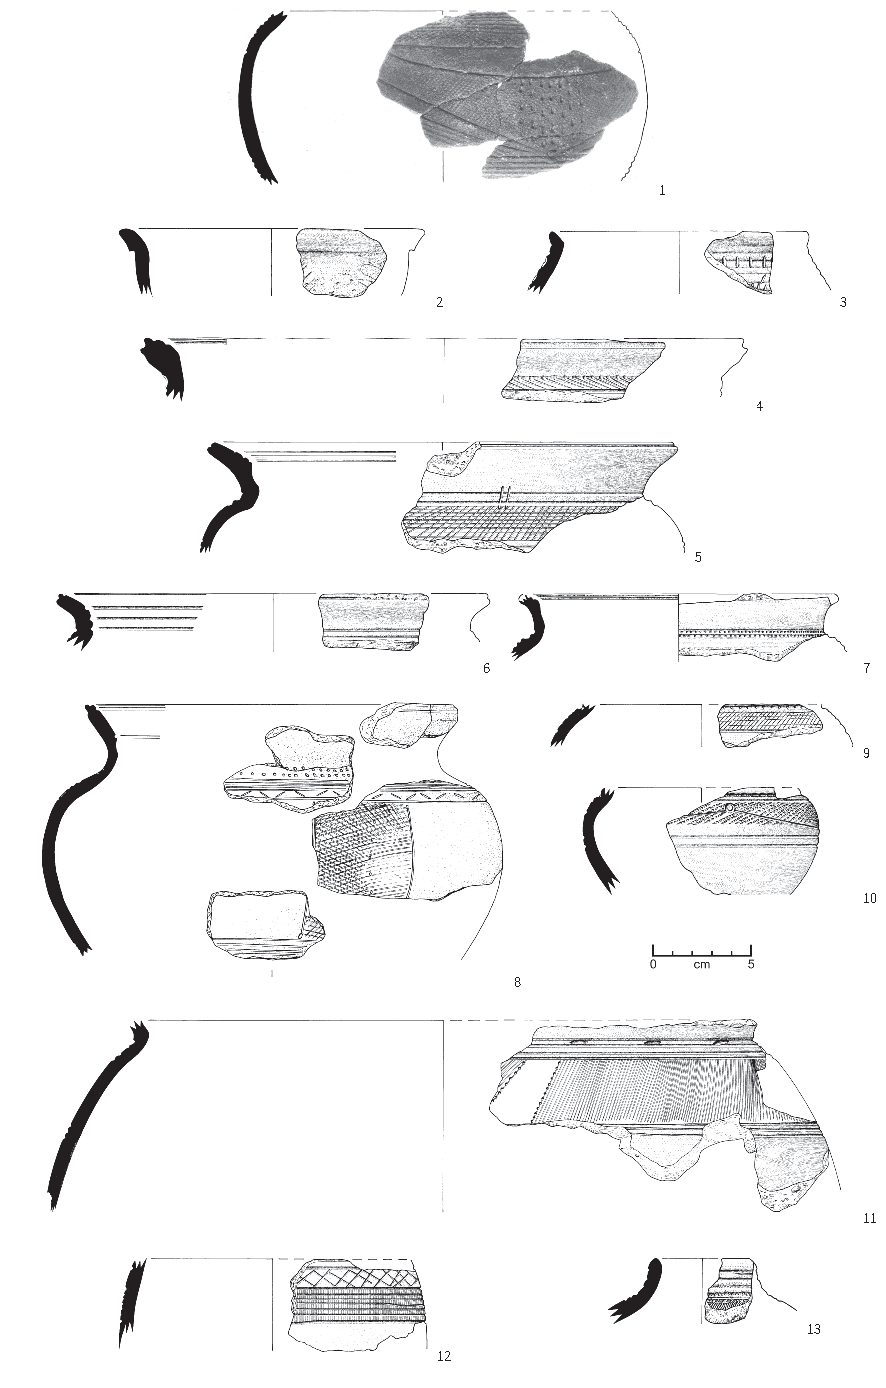
\includegraphics{plt/Taf25.pdf}
	\vspace{.75em}\caption{Lua, Grabungs- \& Oberflächenfunde (1) \\ 1 MLB~85/102; 2--13 MLB~85/1-3-1.}
	\label{pl:25}
\end{pl}

\begin{pl}[H]
	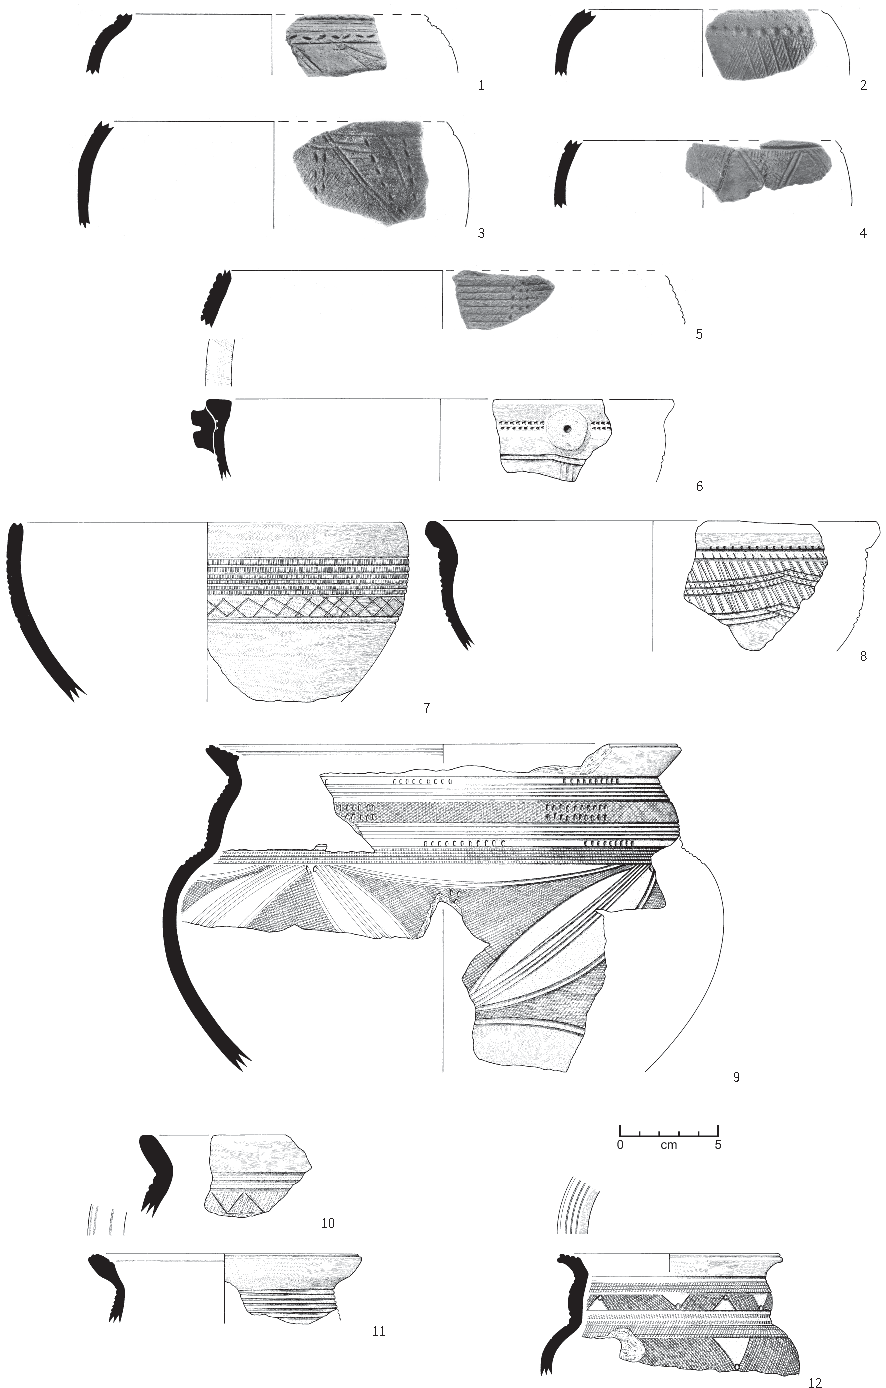
\includegraphics{plt/Taf26.pdf}
	\vspace{.75em}\caption{Lua, Grabungs- \& Oberflächenfunde (9) \\ 1--8 MLB~85/1-3-1; 9 MLB~85/104; 10--12 MLB~85/1-3-2.}
	\label{pl:26}
\end{pl}

\begin{pl}[H]
	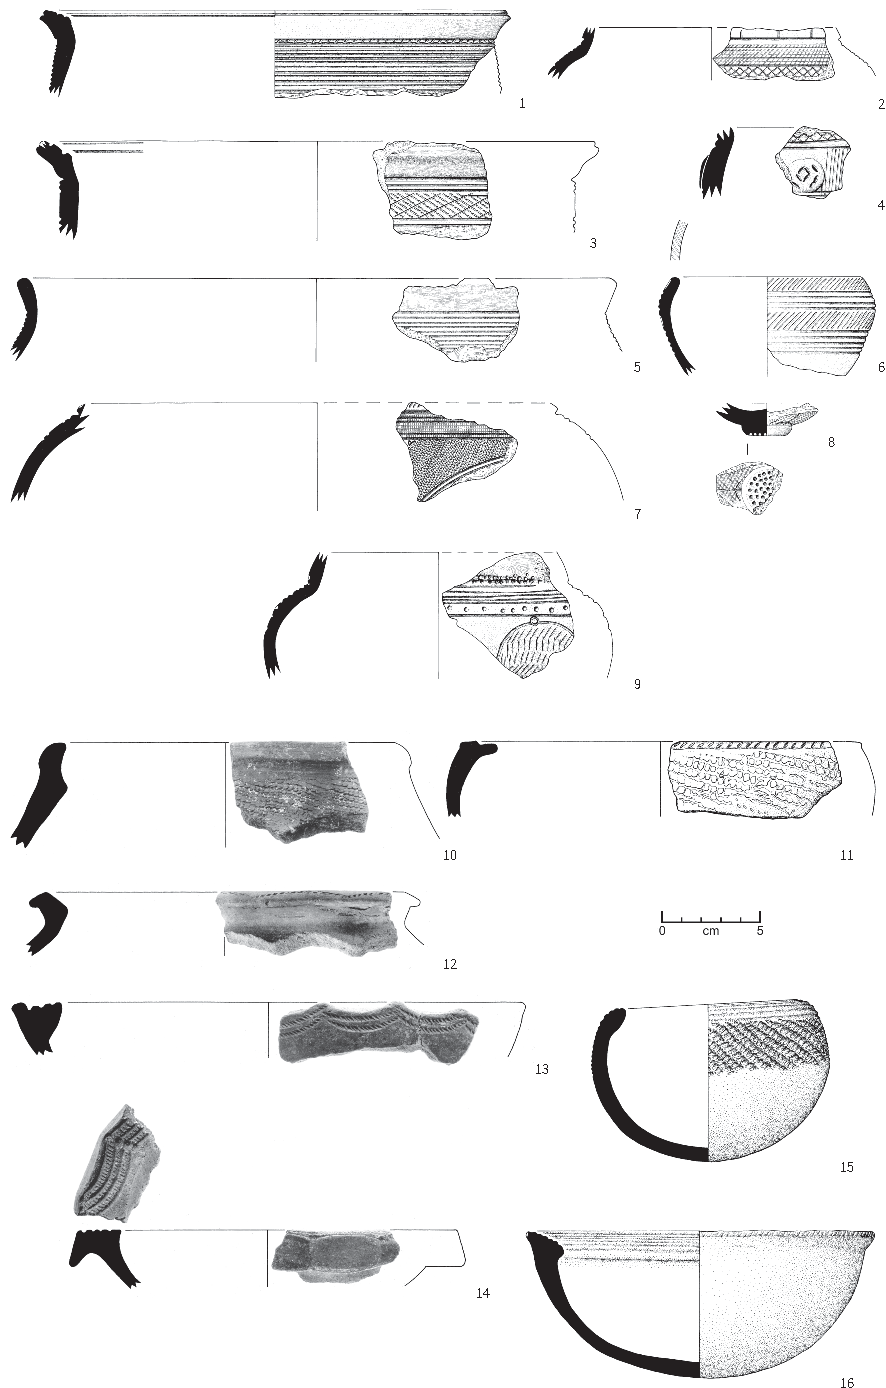
\includegraphics{plt/Taf27.pdf}
	\vspace{.75em}\caption{Lua, Grabungsfunde \& Ankauf (15--16) \\ 1--8 MLB~85/1-3-2; 9 MLB~85/1-4-3; 10--13 MLB~85/103; 14 ILW~85/101; 15--16 ILW~85/501.}
	\label{pl:27}
\end{pl}

\begin{pl}[H]
	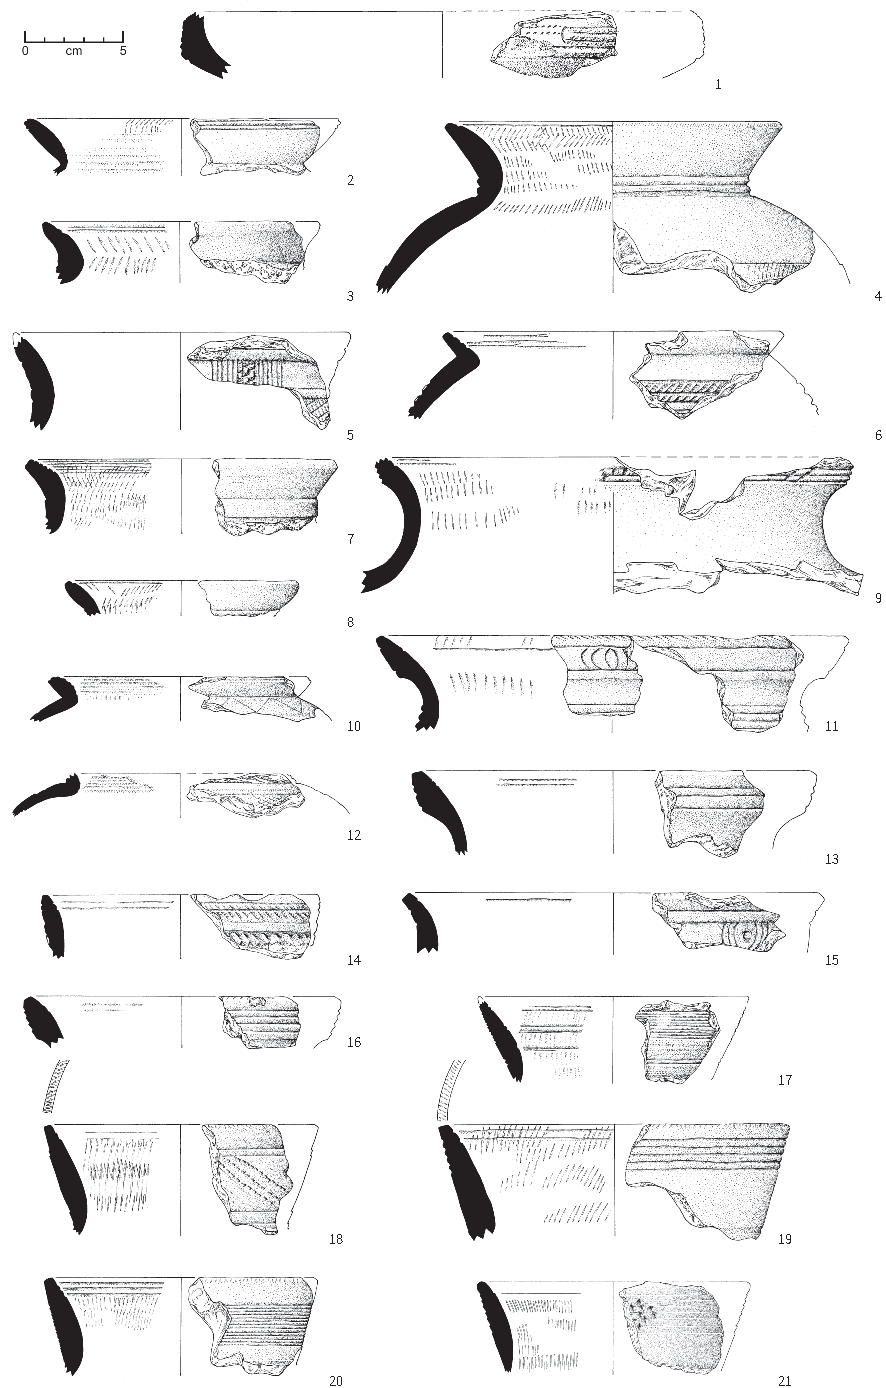
\includegraphics{plt/Taf28.pdf}
	\vspace{.75em}\caption{Kongo, Oberflächenfunde \\ 1 LUZ~87/101; 2--22 MBR~87/101.}
	\label{pl:28}
\end{pl}

\begin{pl}[H]
	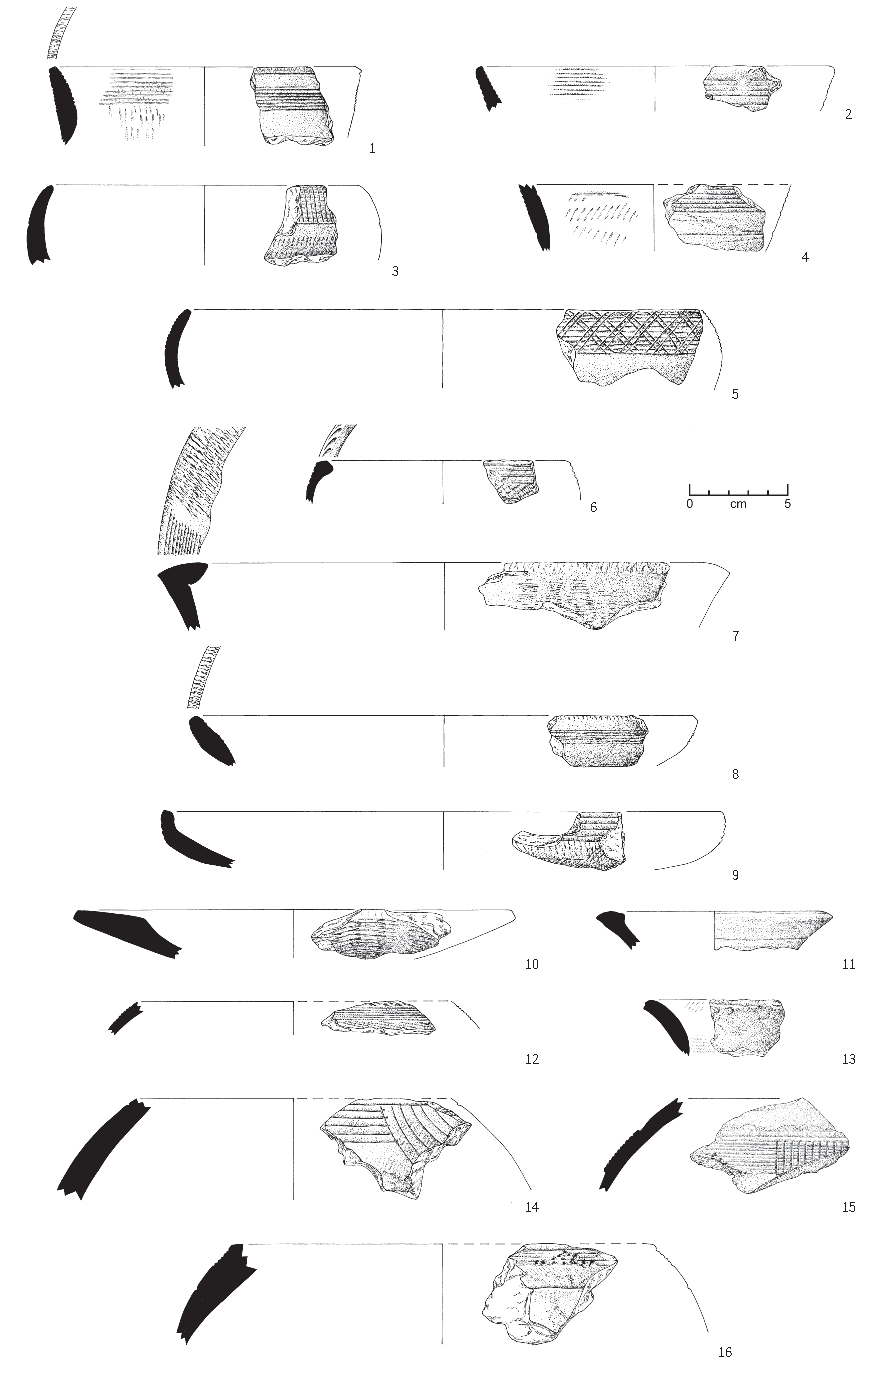
\includegraphics{plt/Taf29.pdf}
	\vspace{.75em}\caption{Kongo, Oberflächenfunde \\ 1--16 MBR~87/101.}
	\label{pl:29}
\end{pl}

\begin{pl}[H]
	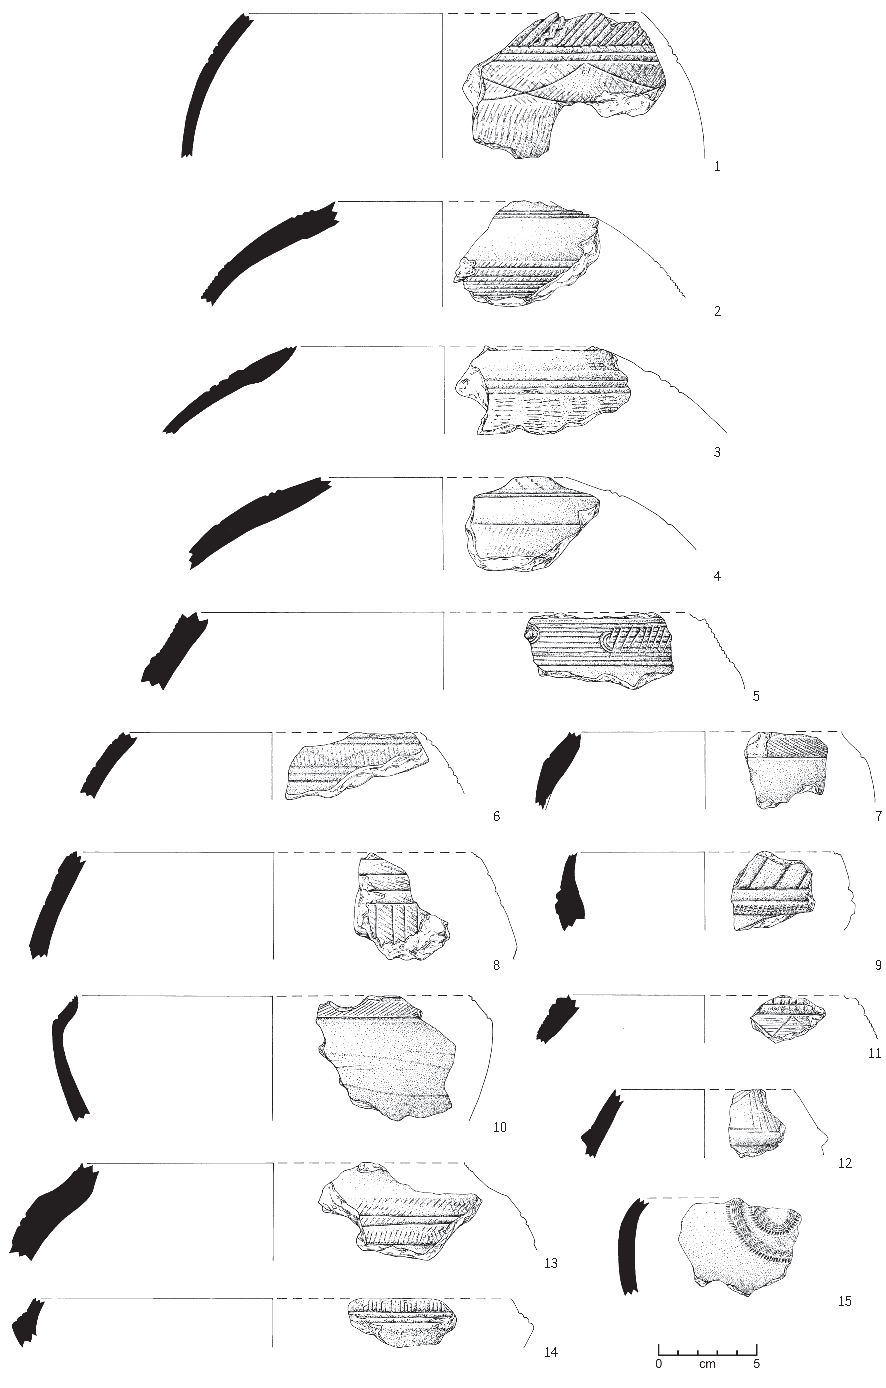
\includegraphics{plt/Taf30.pdf}
	\vspace{.75em}\caption{Kongo, Oberflächenfunde \\ 1--15 MBR~87/101.}
	\label{pl:30}
\end{pl}

\begin{pl}[H]
	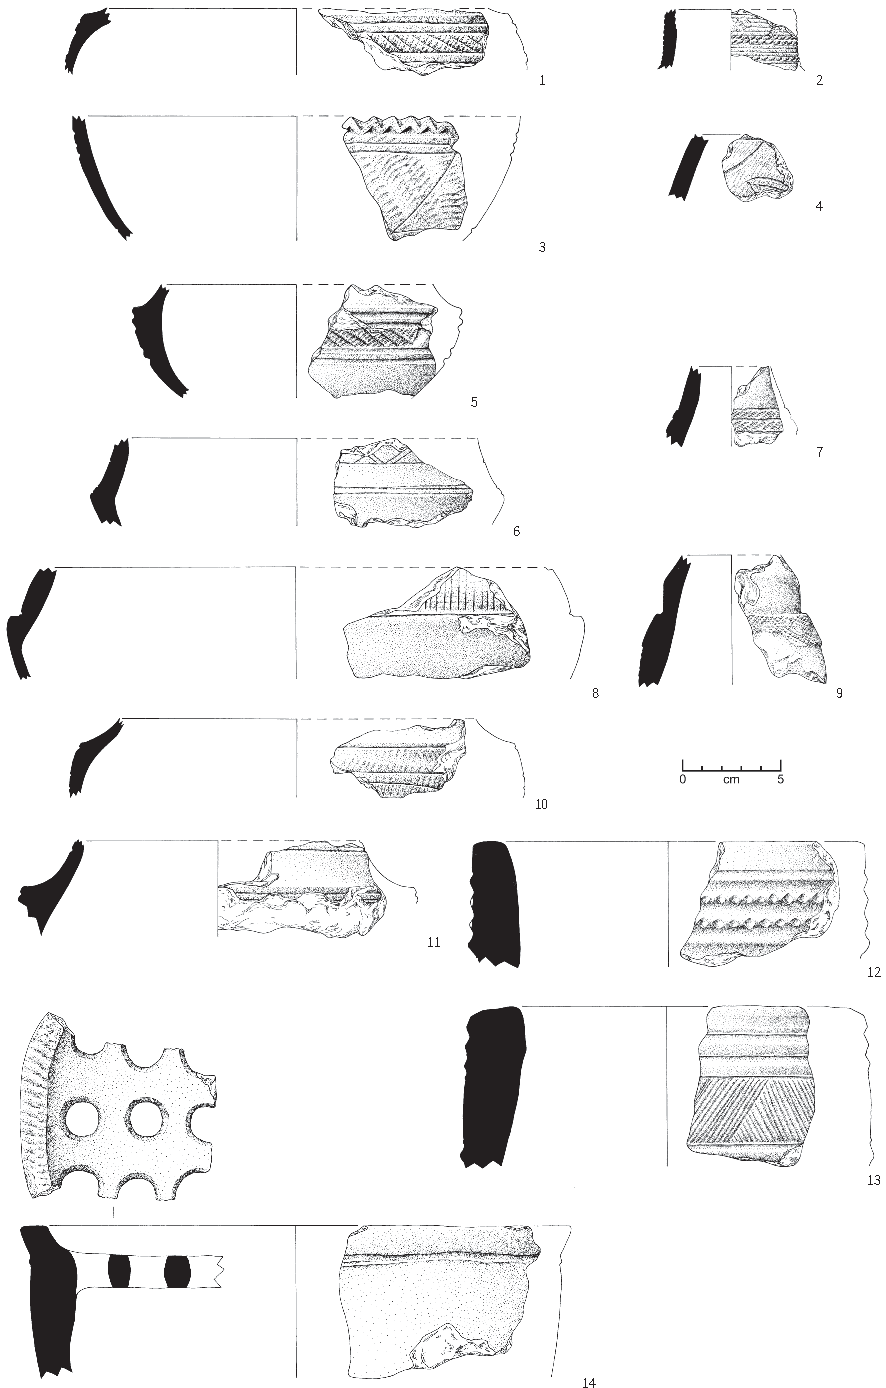
\includegraphics{plt/Taf31.pdf}
	\vspace{.75em}\caption{Kongo, Oberflächenfunde \\ 1--14 MBR~87/101.}
	\label{pl:31}
\end{pl}

\begin{pl}[H]
	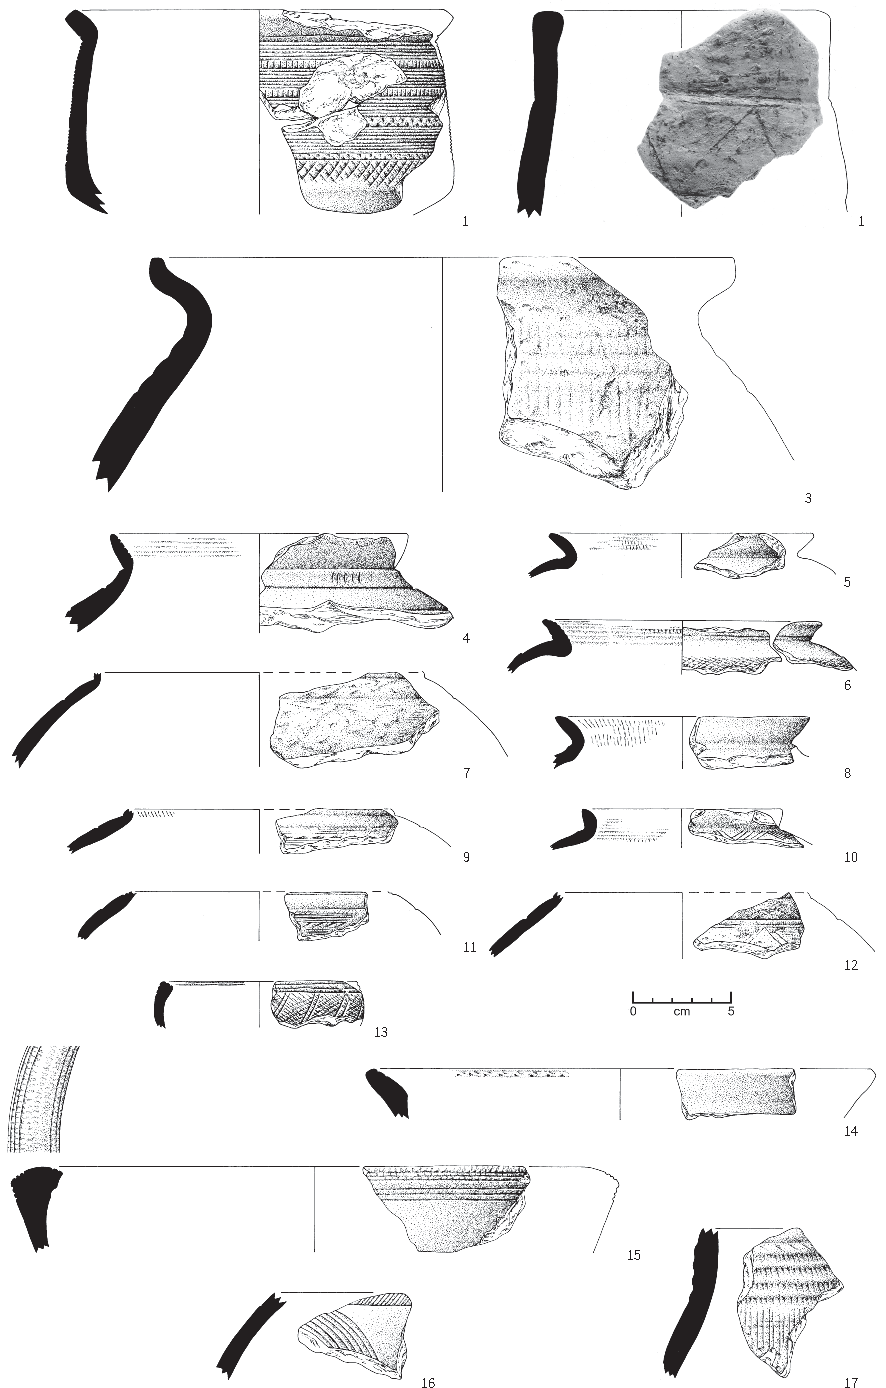
\includegraphics{plt/Taf32.pdf}
	\vspace{.75em}\caption{Kongo, Oberflächenfunde \\ 1--17 SUN~87/101.}
	\label{pl:32}
\end{pl}

\begin{pl}[H]
	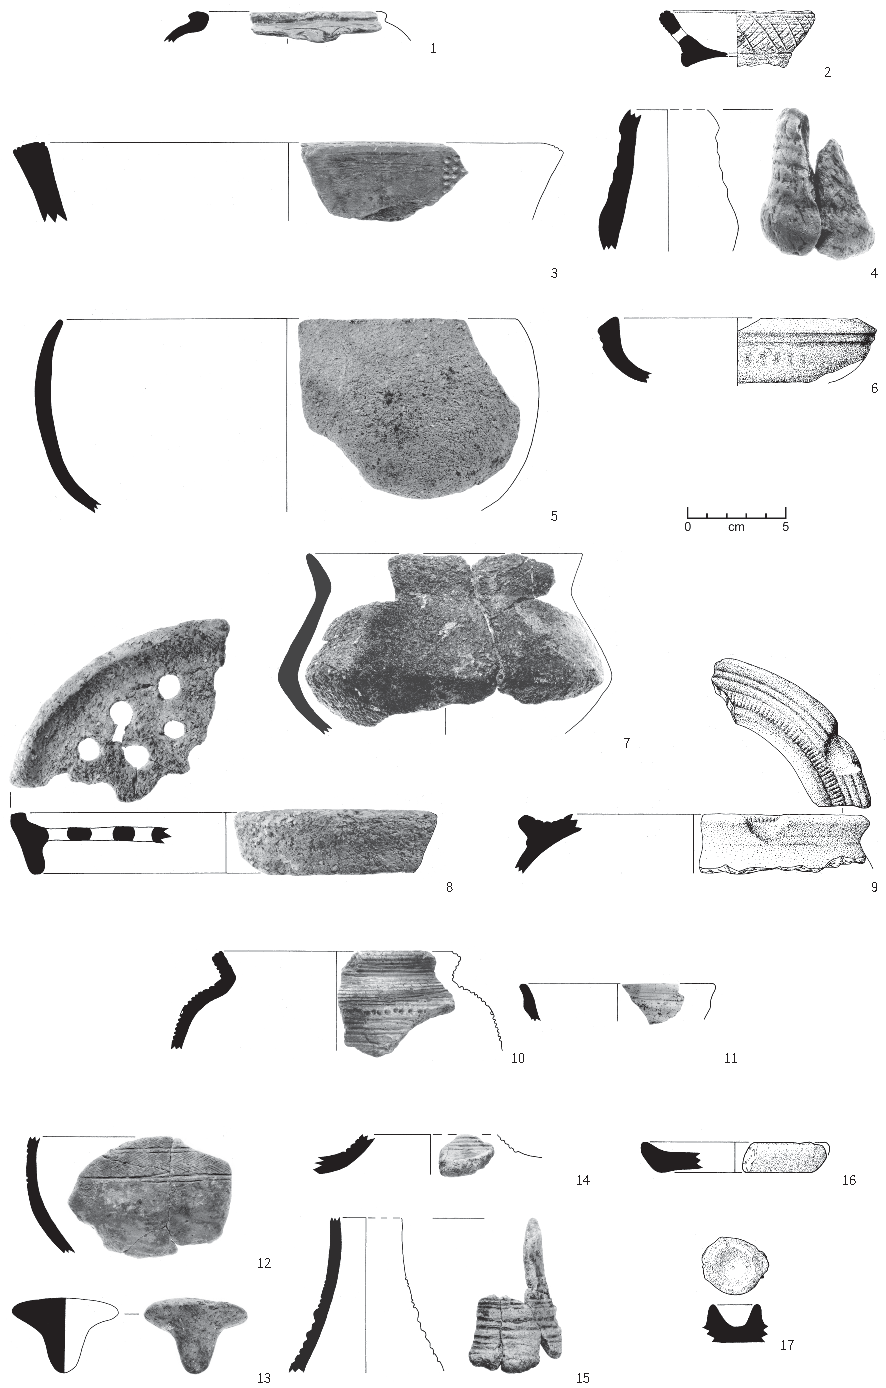
\includegraphics{plt/Taf33.pdf}
	\vspace{.75em}\caption{Kongo \& \mbox{Sangha}, Grabungs- \& Oberflächenfunde (1--10) \\ 1--5 GMB~87/101; 6--10 BGA~87/101; 11--12 BGA~87/102; 13--16 BBS~87/1; 17--18 BBS~87/2.}
	\label{pl:33}
\end{pl}

\begin{pl}[H]
	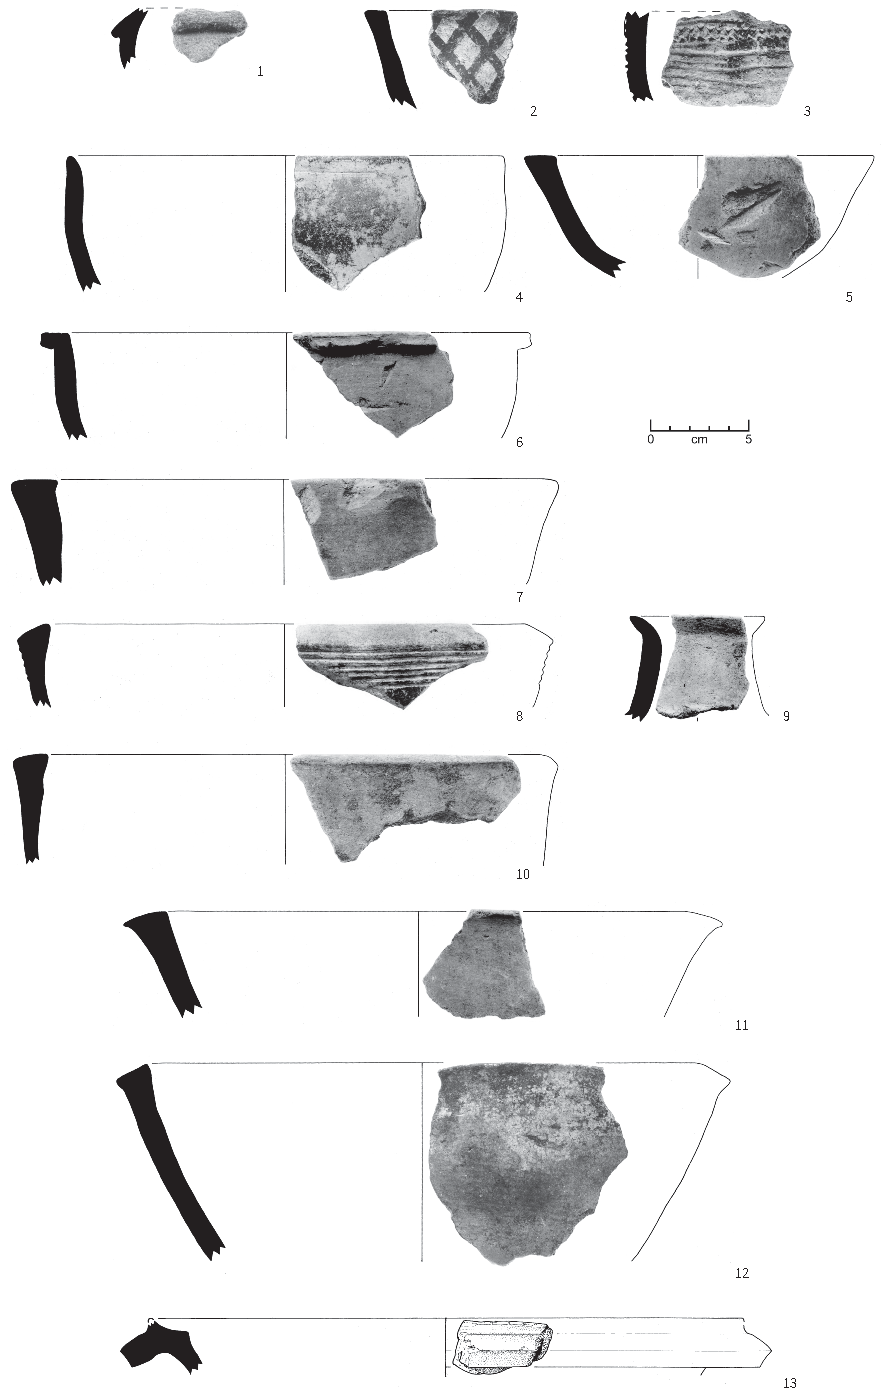
\includegraphics{plt/Taf34.pdf}
	\vspace{.75em}\caption{\mbox{Sangha}, Oberflächenfunde \\ 1--3 BBS~87/101; 4--14 BBS~87/102.}
	\label{pl:34}
\end{pl}

\begin{pl}[H]
	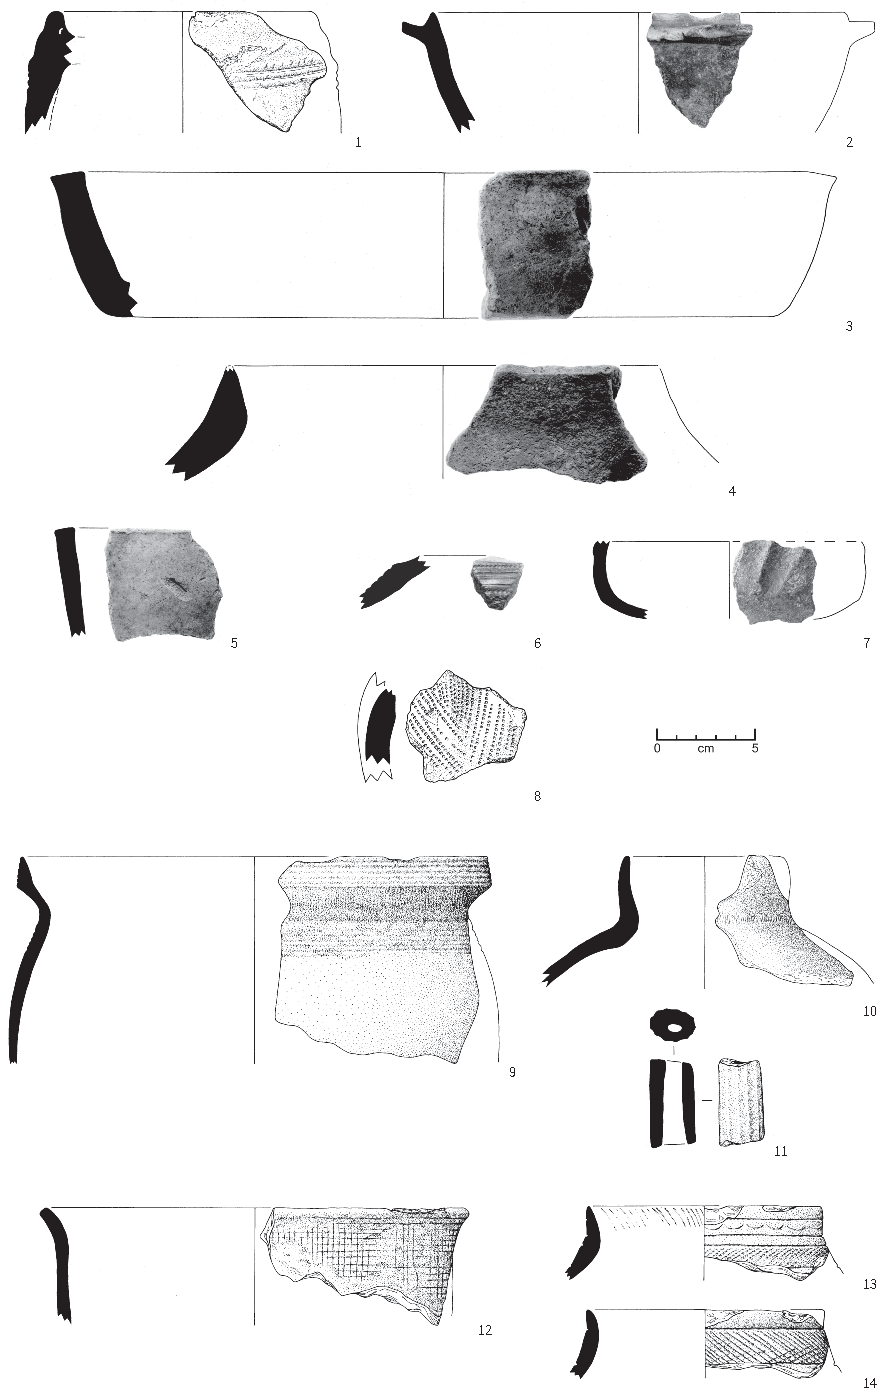
\includegraphics{plt/Taf35.pdf}
	\vspace{.75em}\caption{\mbox{Sangha}, Oberflächenfunde \\ 1--9 BBS~87/102; 10--12 SGH~87/040; 13--15 SSL~87/101.}
	\label{pl:35}
\end{pl}

\begin{pl}[H]
	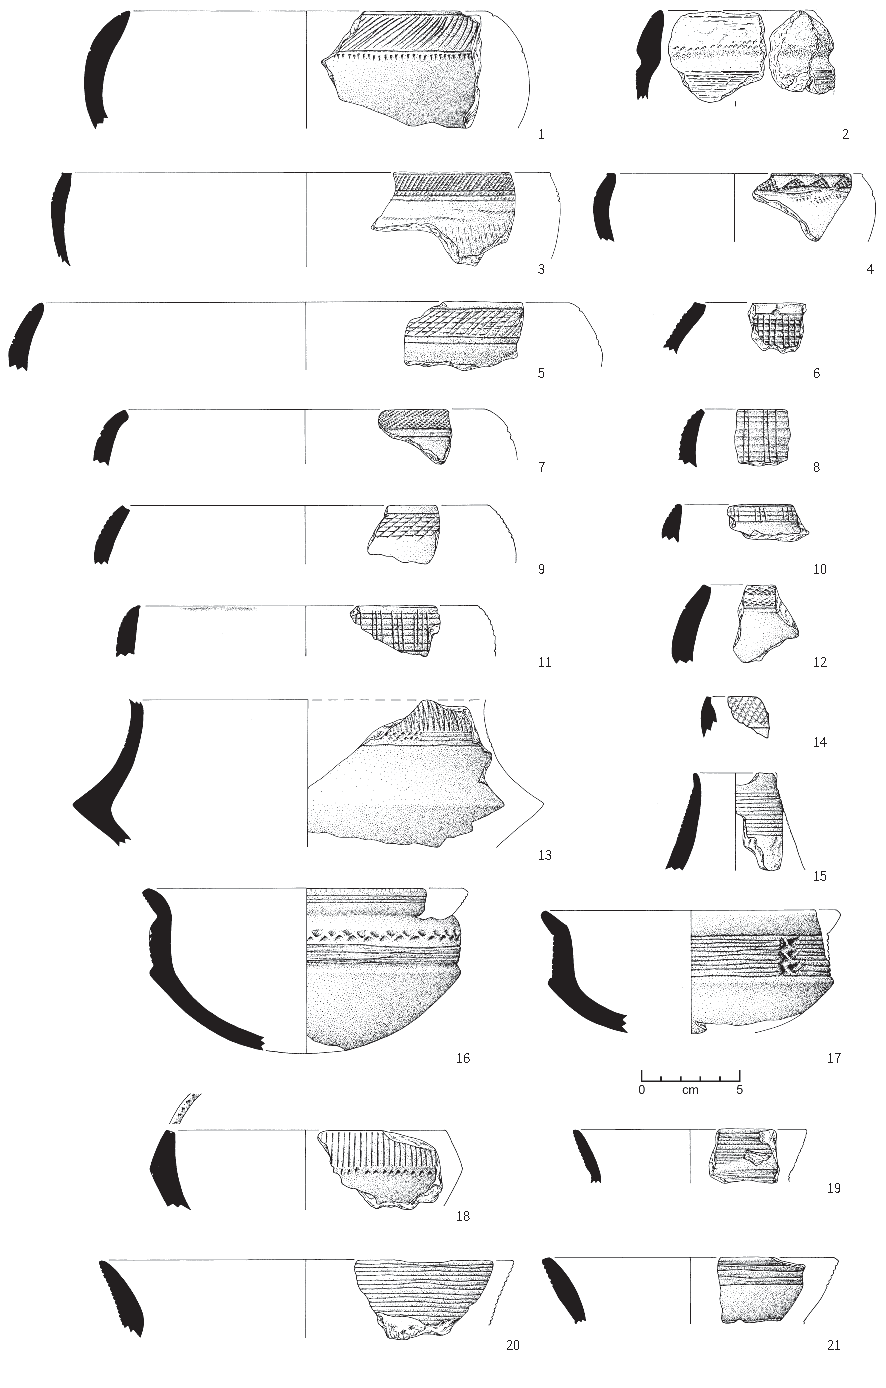
\includegraphics{plt/Taf36.pdf}
	\vspace{.75em}\caption{\mbox{Sangha}, Oberflächenfunde \\ 1--21 SSL~87/101.}
	\label{pl:36}
\end{pl}

\begin{pl}[H]
	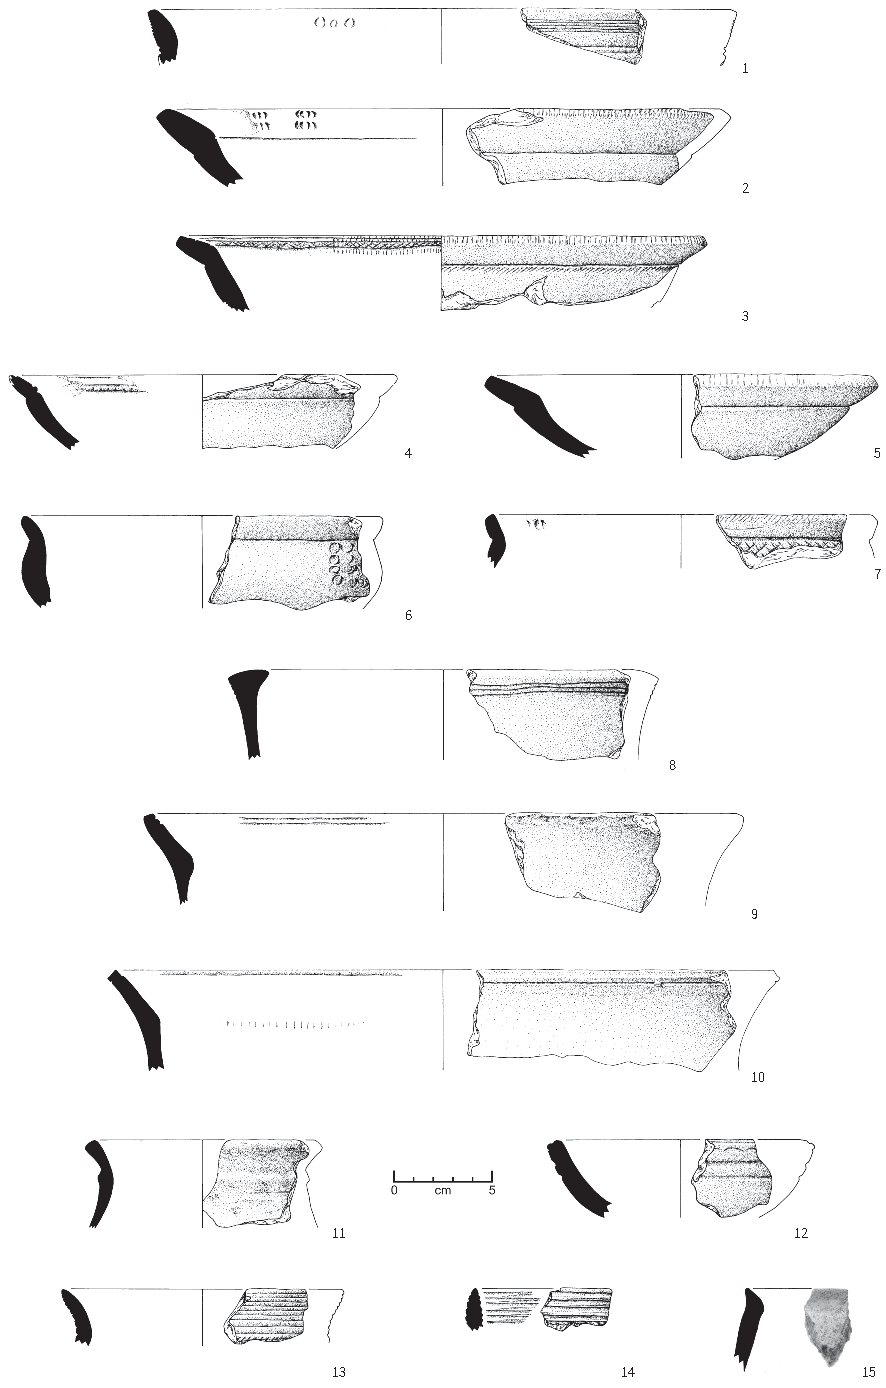
\includegraphics{plt/Taf37.pdf}
	\vspace{.75em}\caption{\mbox{Sangha}, Oberflächenfunde \\ 1--17 SSL~87/101.}
	\label{pl:37}
\end{pl}

\begin{pl}[H]
	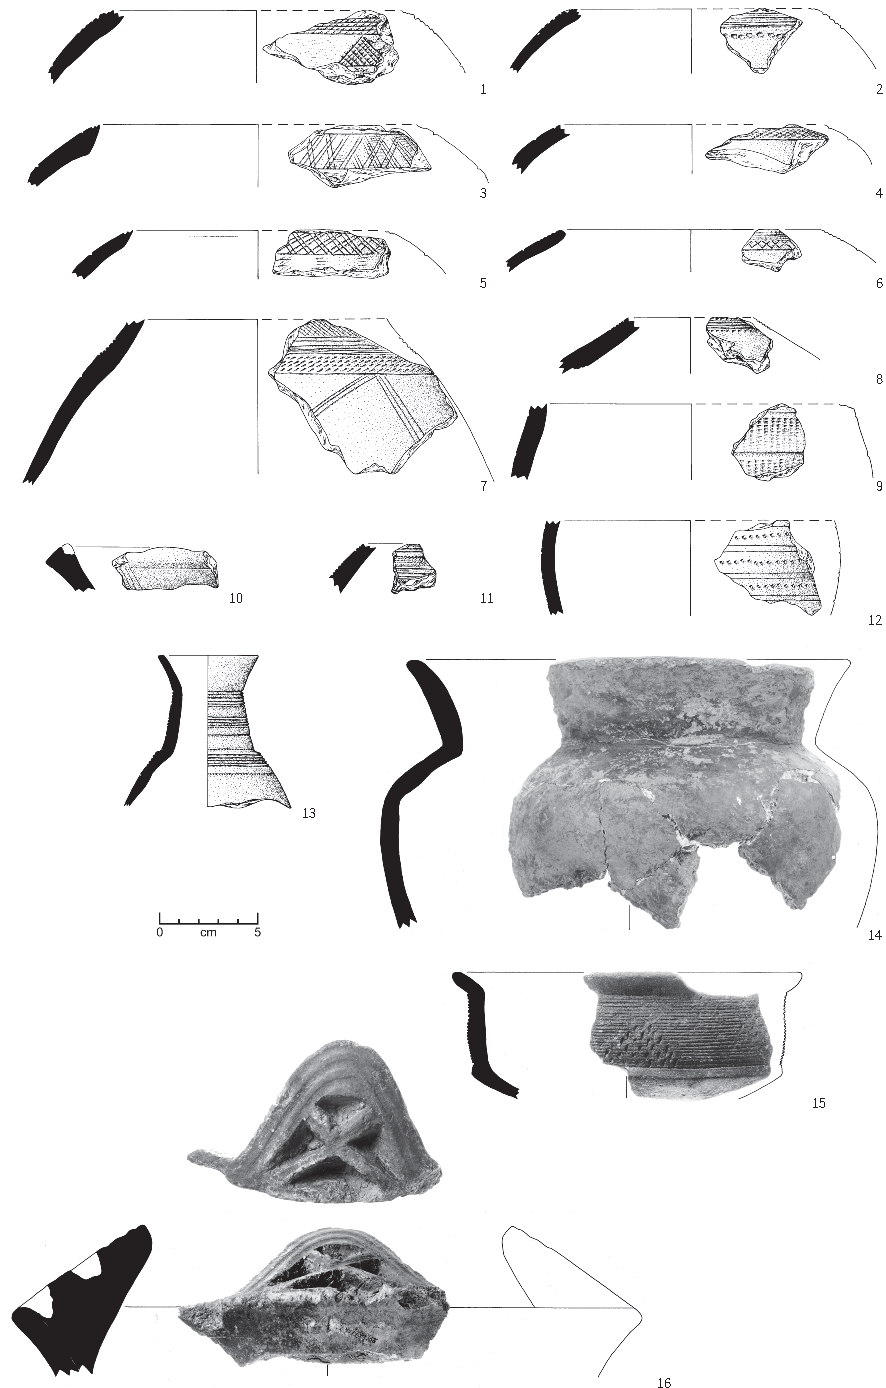
\includegraphics{plt/Taf38.pdf}
	\vspace{.75em}\caption{\mbox{Sangha}, Oberflächenfunde \\ 1--12 SSL~87/101; 13 SGH~87/072; 14--16 MJL~87/101.}
	\label{pl:38}
\end{pl}

\begin{pl}[H]
	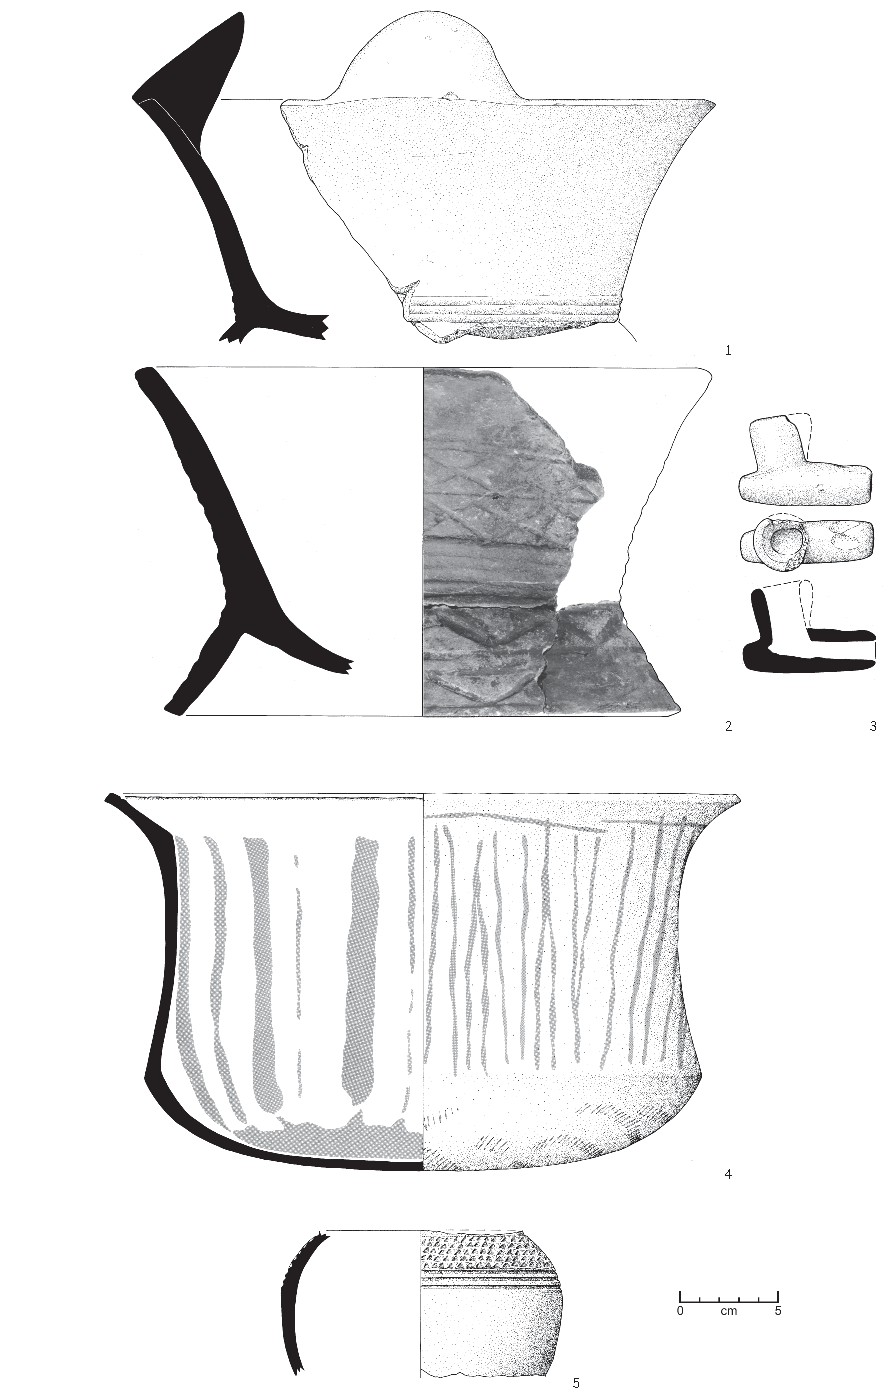
\includegraphics{plt/Taf39.pdf}
	\vspace{.75em}\caption{\mbox{Sangha}, Oberflächenfunde \\ 1--3 MJL~87/101; 4 MKA~87/101; 5 MKA~87/102.}
	\label{pl:39}
\end{pl}

\begin{pl}[H]
	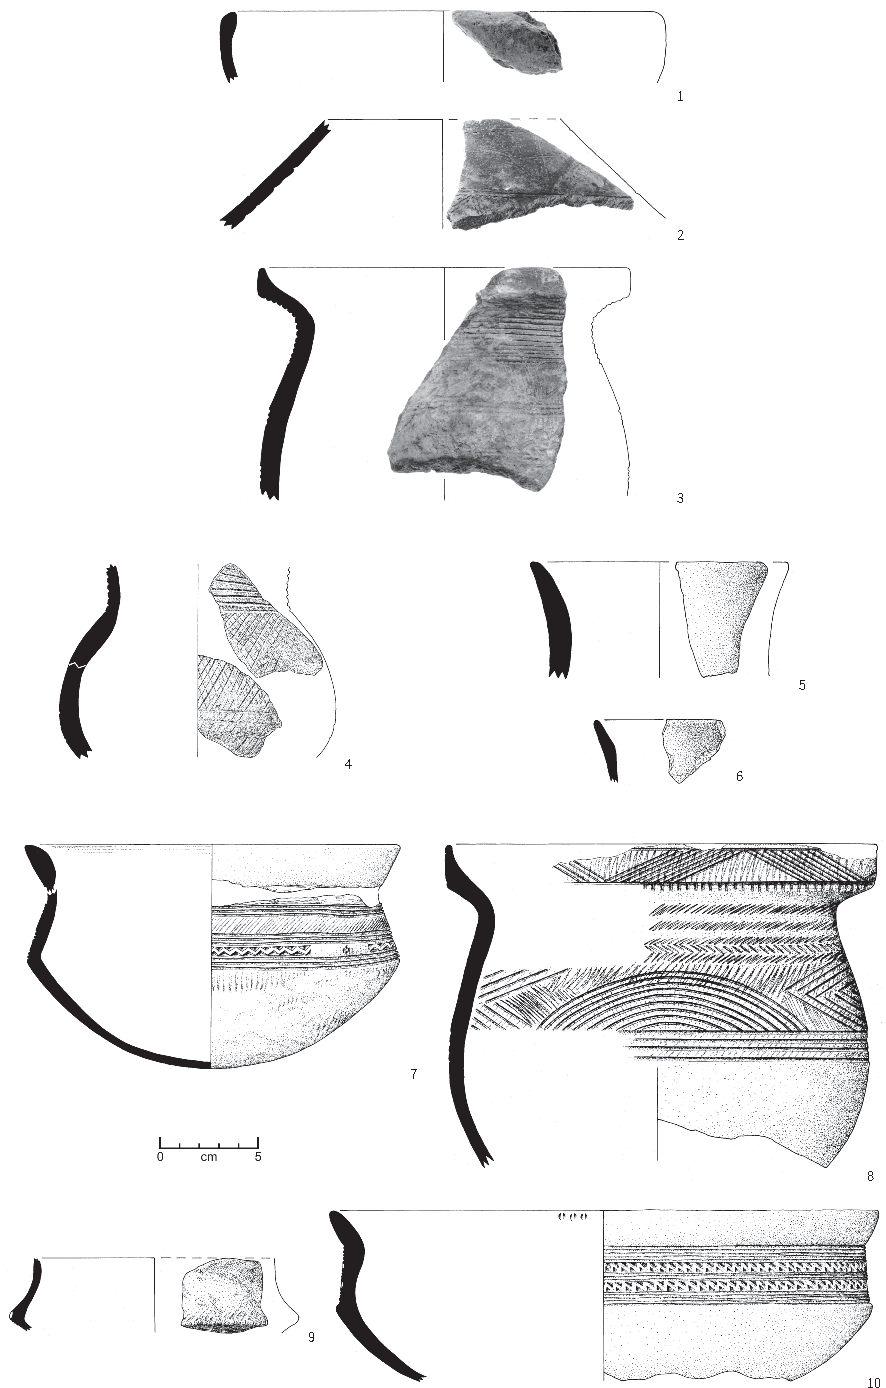
\includegraphics{plt/Taf40.pdf}
	\vspace{.75em}\caption{\mbox{Sangha}, Oberflächenfunde \\ 1--5 LBK~87/101; 6--8 INS~87/101; 9 INS~87/102; 10 BOG~87/101; 11--12 BOG~87/102.}
	\label{pl:40}
\end{pl}

\begin{pl}[H]
	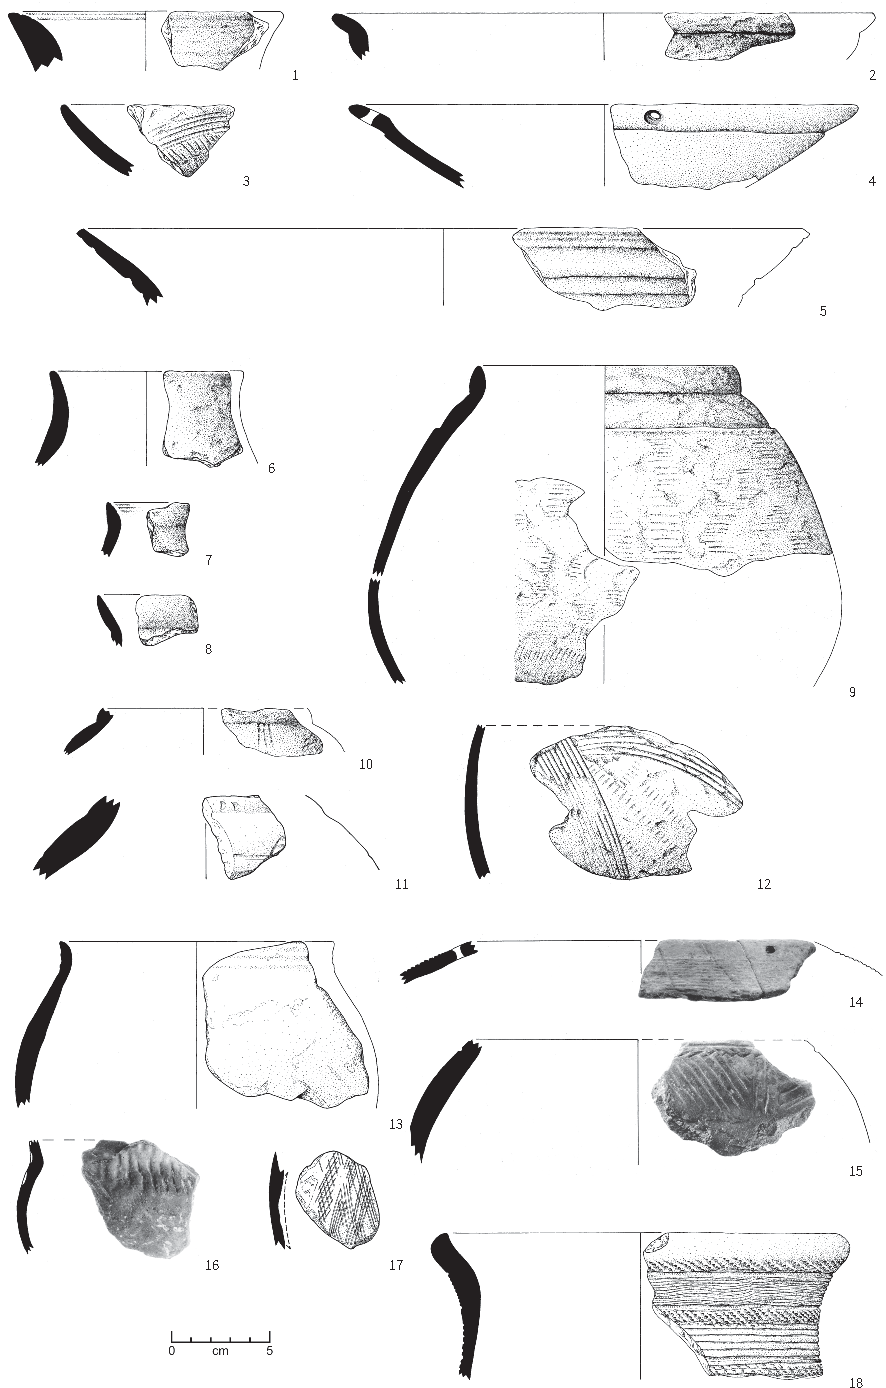
\includegraphics{plt/Taf41.pdf}
	\vspace{.75em}\caption{\mbox{Sangha}, Oberflächenfunde \\ 1--5 BOG~87/102; 6--12 BOG~87/103; 13--17 MIT~87/101; 18 MIT~87/102.}
	\label{pl:41}
\end{pl}

\begin{pl}[H]
	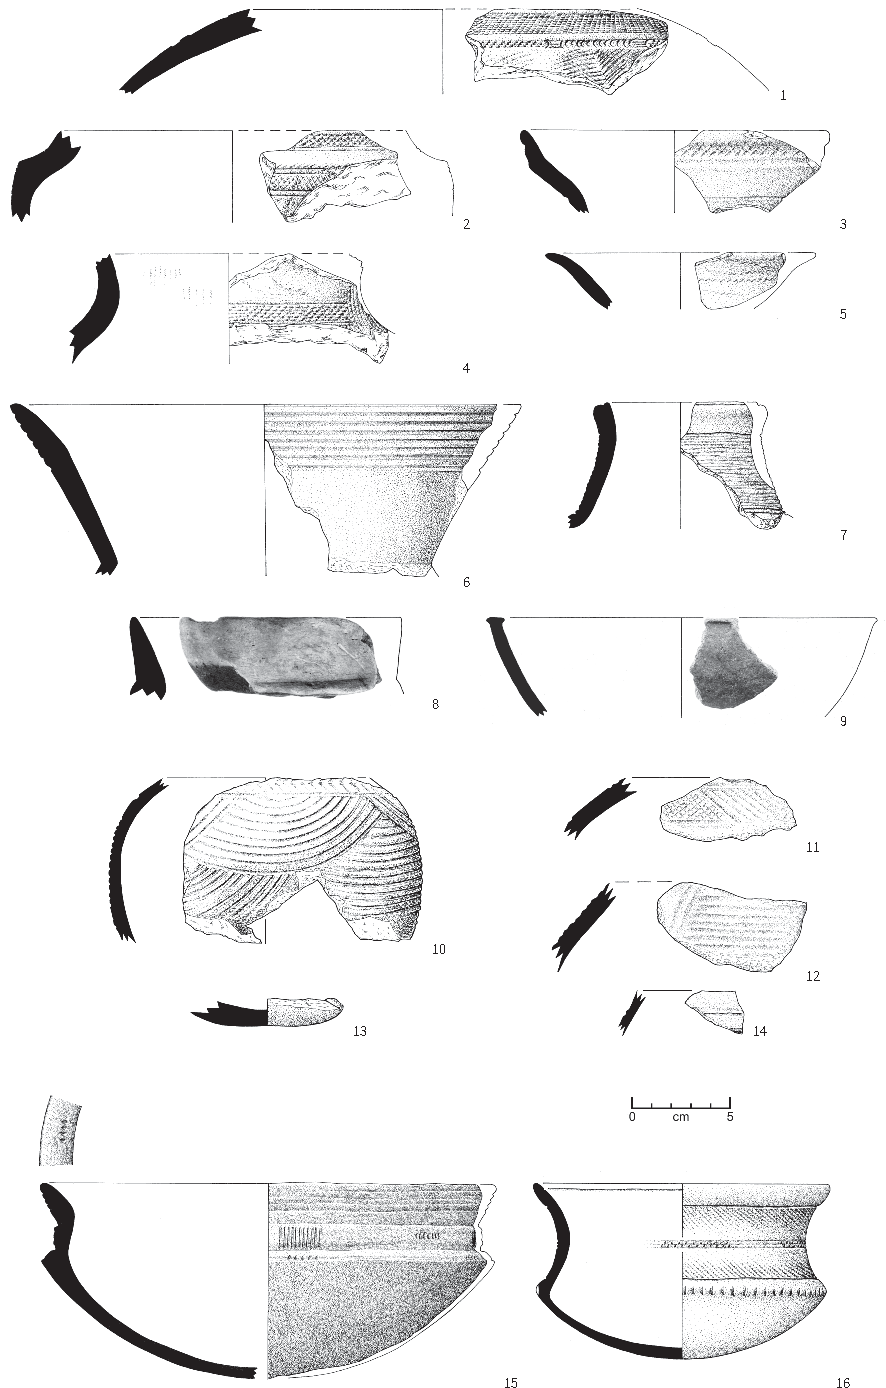
\includegraphics{plt/Taf42.pdf}
	\vspace{.75em}\caption{\mbox{Sangha}, Grabungs- (10--14) \& Oberflächenfunde \\ 1--9 MIT~87/102; 10--14 MIT~87/103; 15--16 NGO~87/102.}
	\label{pl:42}
\end{pl}

\begin{pl}[H]
	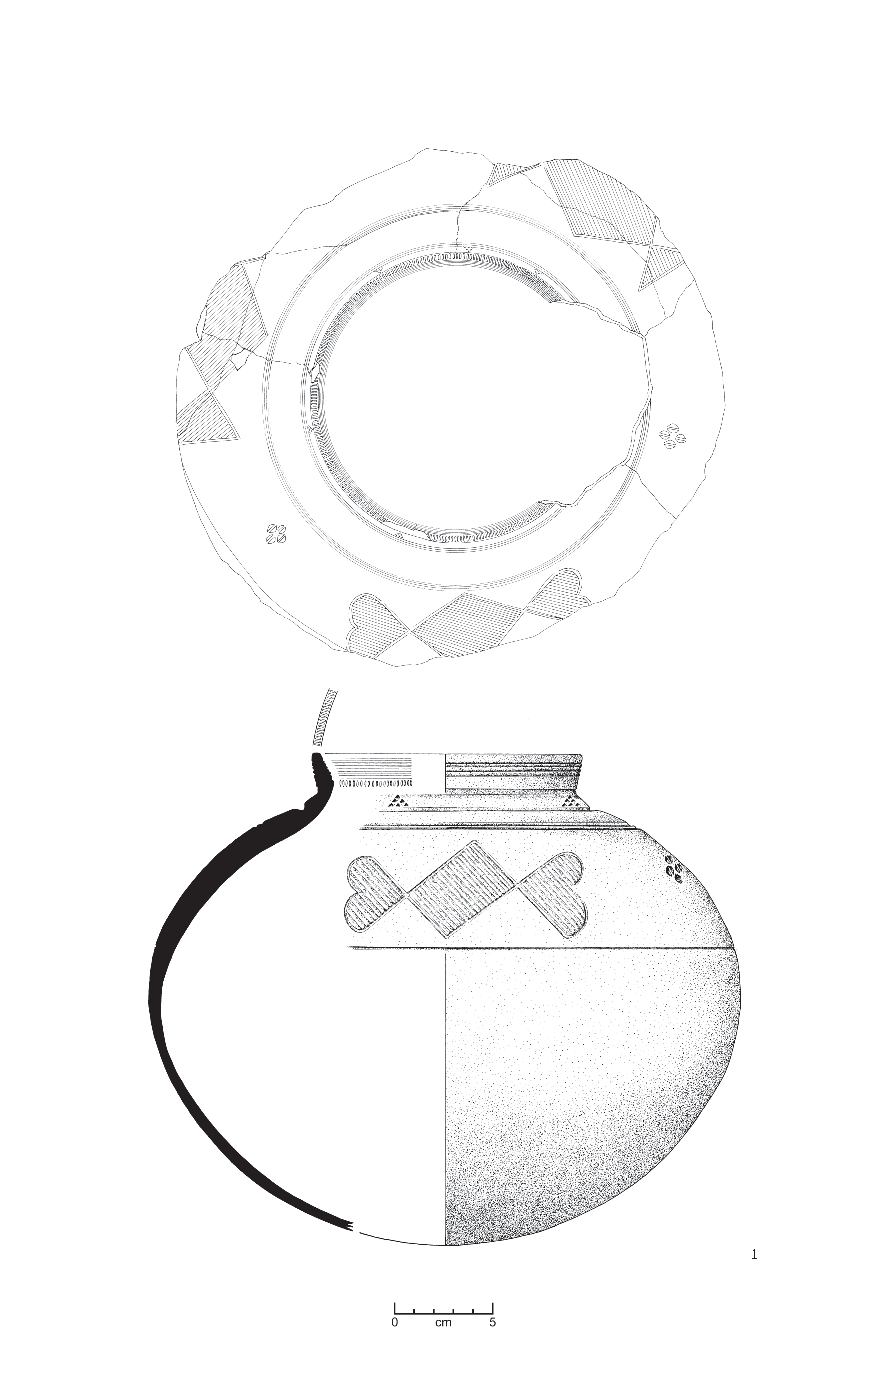
\includegraphics{plt/Taf43.pdf}
	\vspace{.75em}\caption{\mbox{Sangha}, Grabungsfunde \\ 1 NGO~87/102.}
	\label{pl:43}
\end{pl}

\begin{pl}[H]
	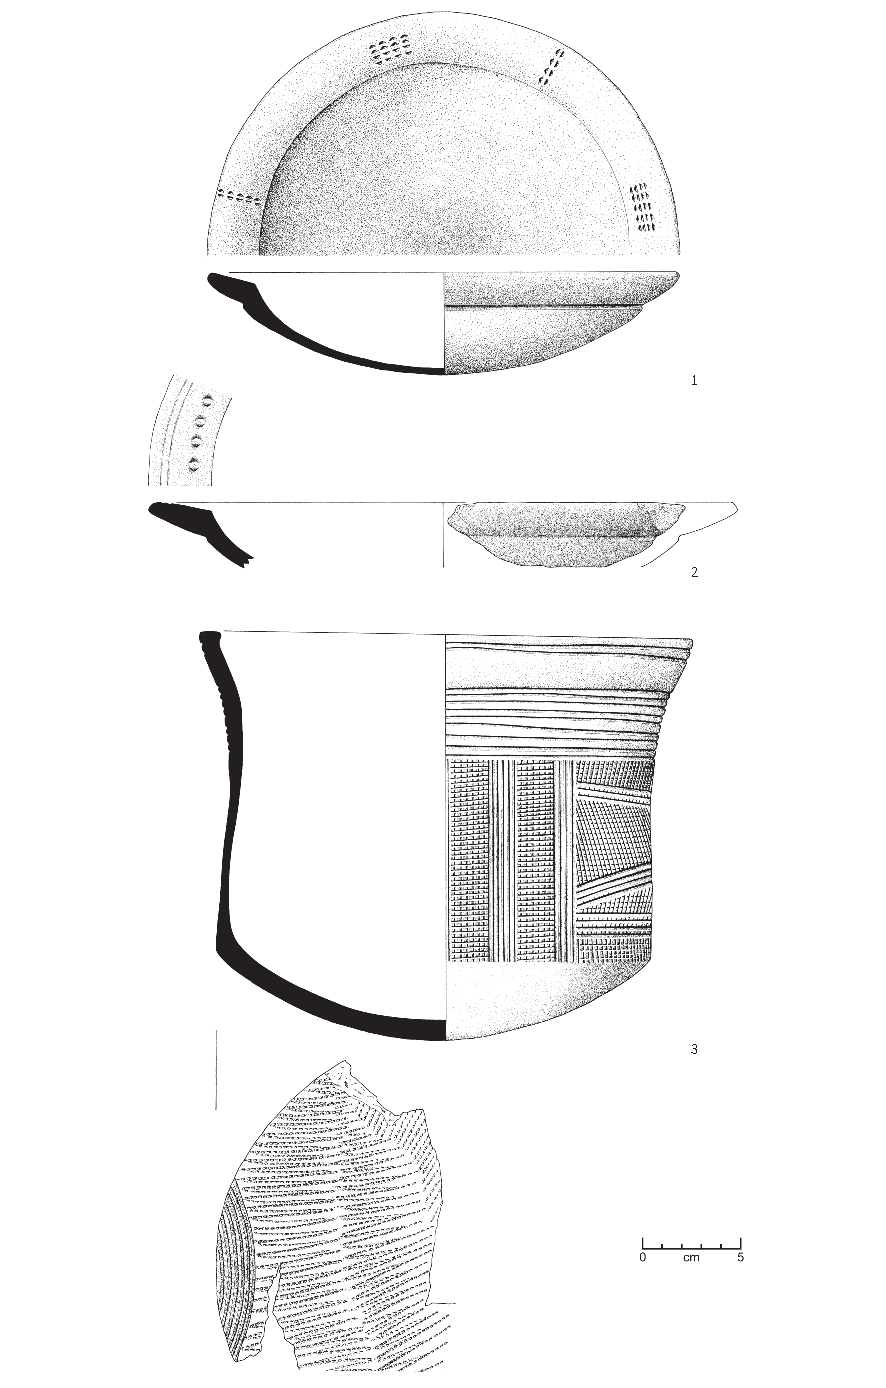
\includegraphics{plt/Taf44.pdf}
	\vspace{.75em}\caption{\mbox{Sangha}, Grabungsfunde \\ 1--2 NGO~87/102; 3 PIK~87/1.}
	\label{pl:44}
\end{pl}

\begin{pl}[H]
	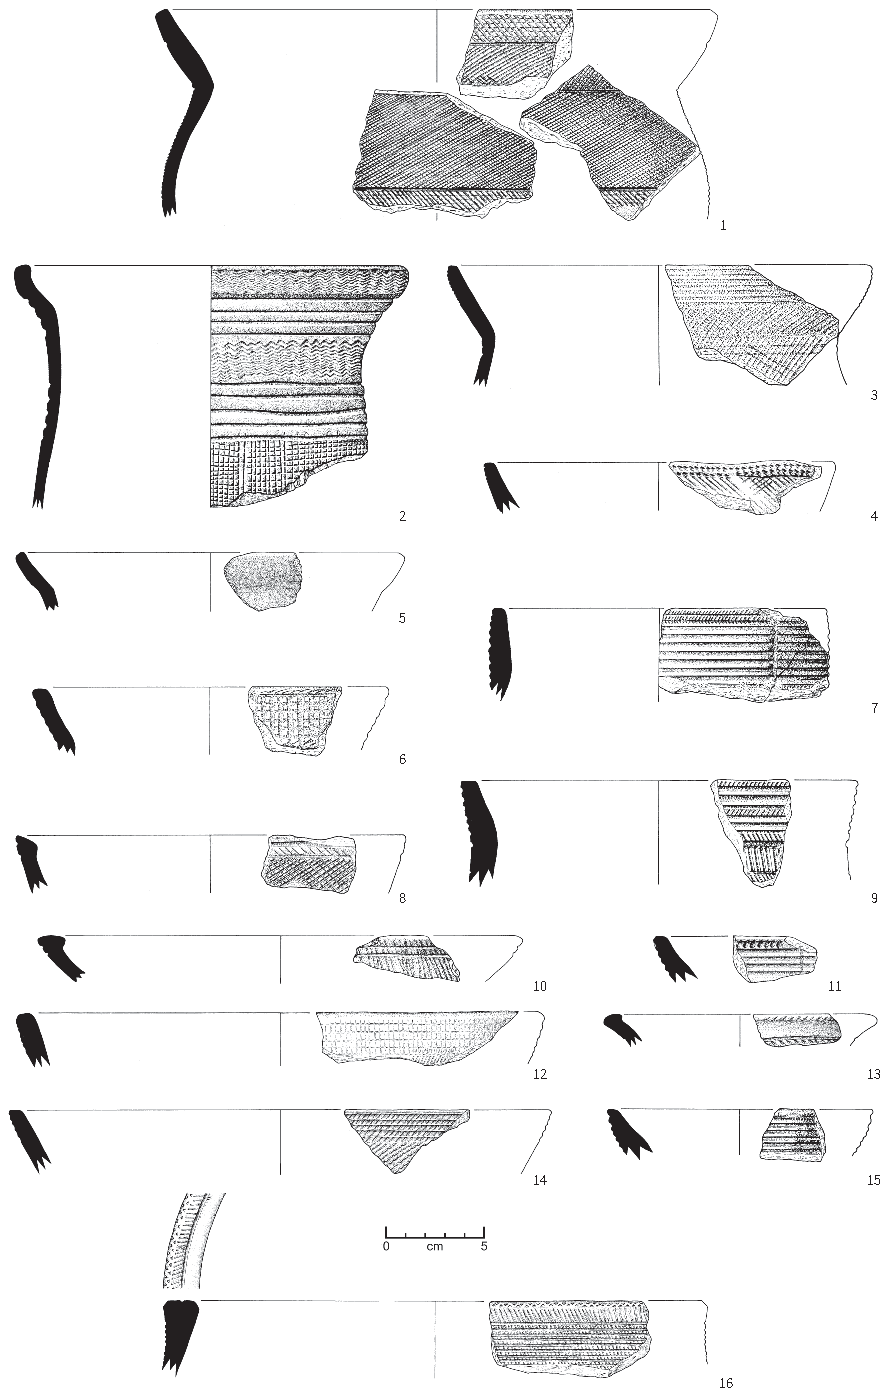
\includegraphics{plt/Taf45.pdf}
	\vspace{.75em}\caption{\mbox{Sangha}, Grabungsfunde \\ 1--17 PIK~87/1.}
	\label{pl:45}
\end{pl}

\begin{pl}[H]
	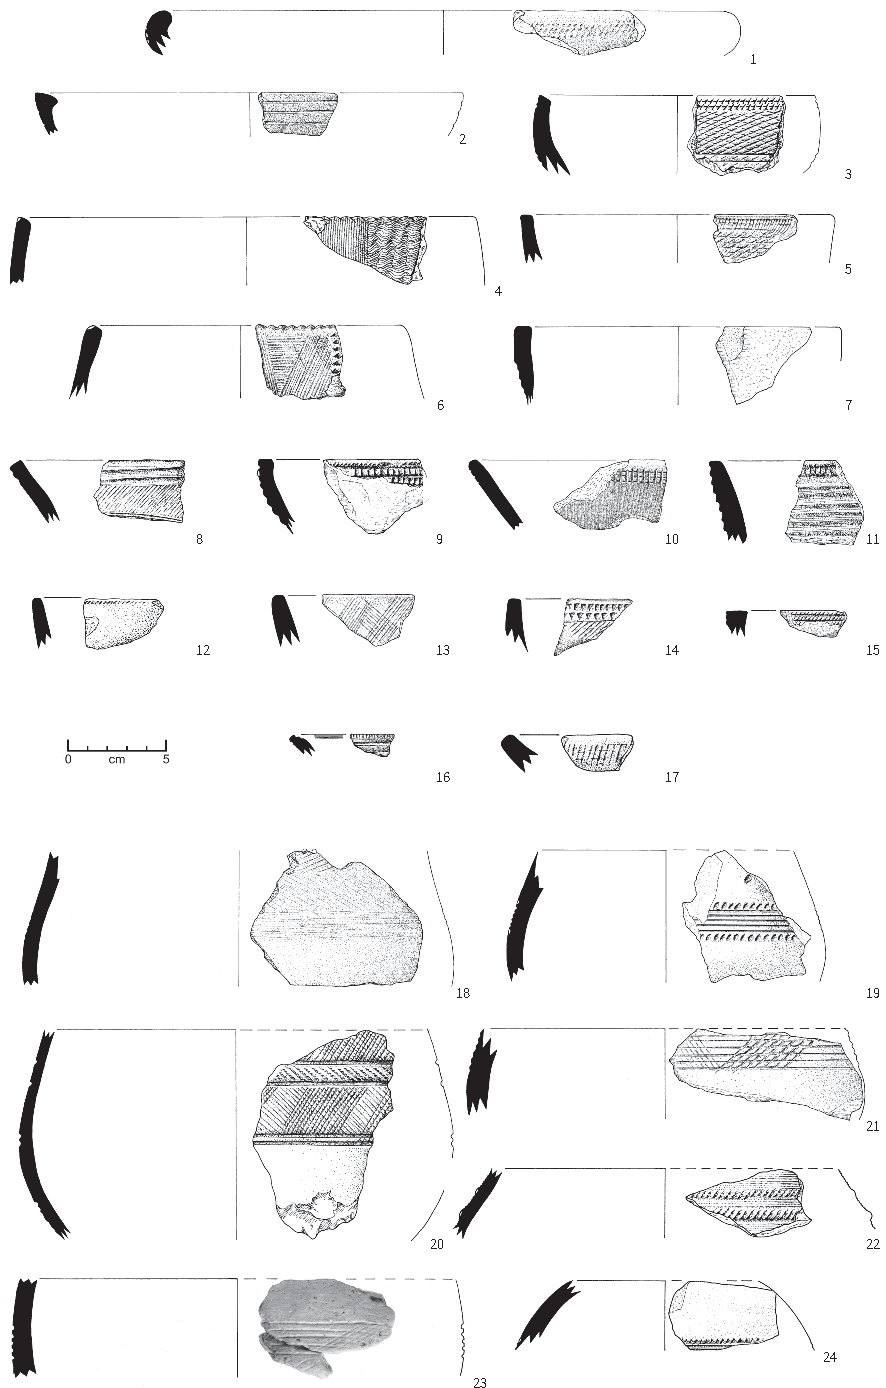
\includegraphics{plt/Taf46.pdf}
	\vspace{.75em}\caption{\mbox{Sangha}, Grabungsfunde \\ 1--26 PIK~87/1.}
	\label{pl:46}
\end{pl}

\begin{pl}[H]
	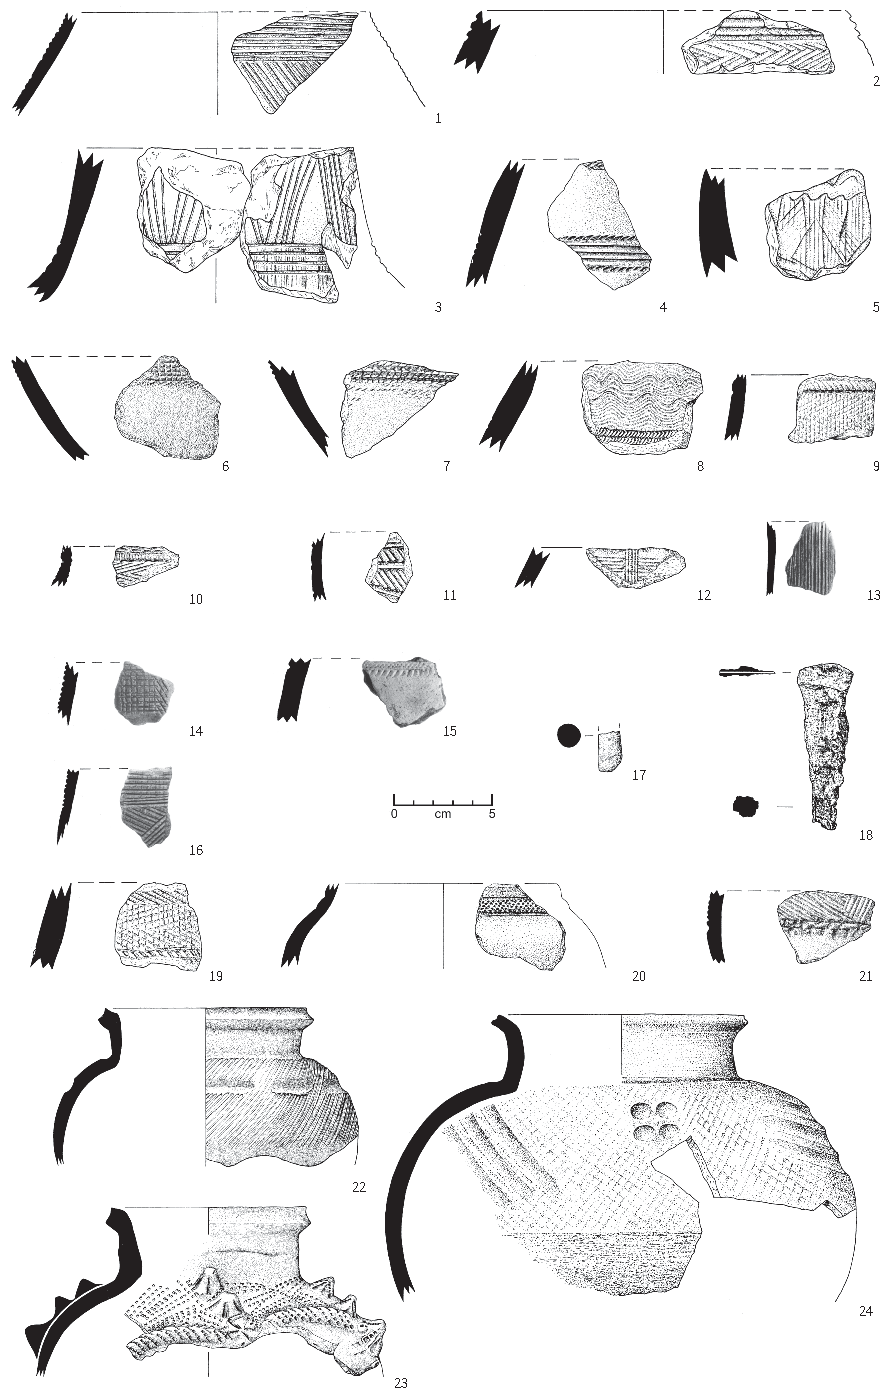
\includegraphics{plt/Taf47.pdf}
	\vspace{.75em}\caption{\mbox{Sangha}, Grabungsfunde \\ 1--25 PIK~87/1.}
	\label{pl:47}
\end{pl}

\begin{pl}[H]
	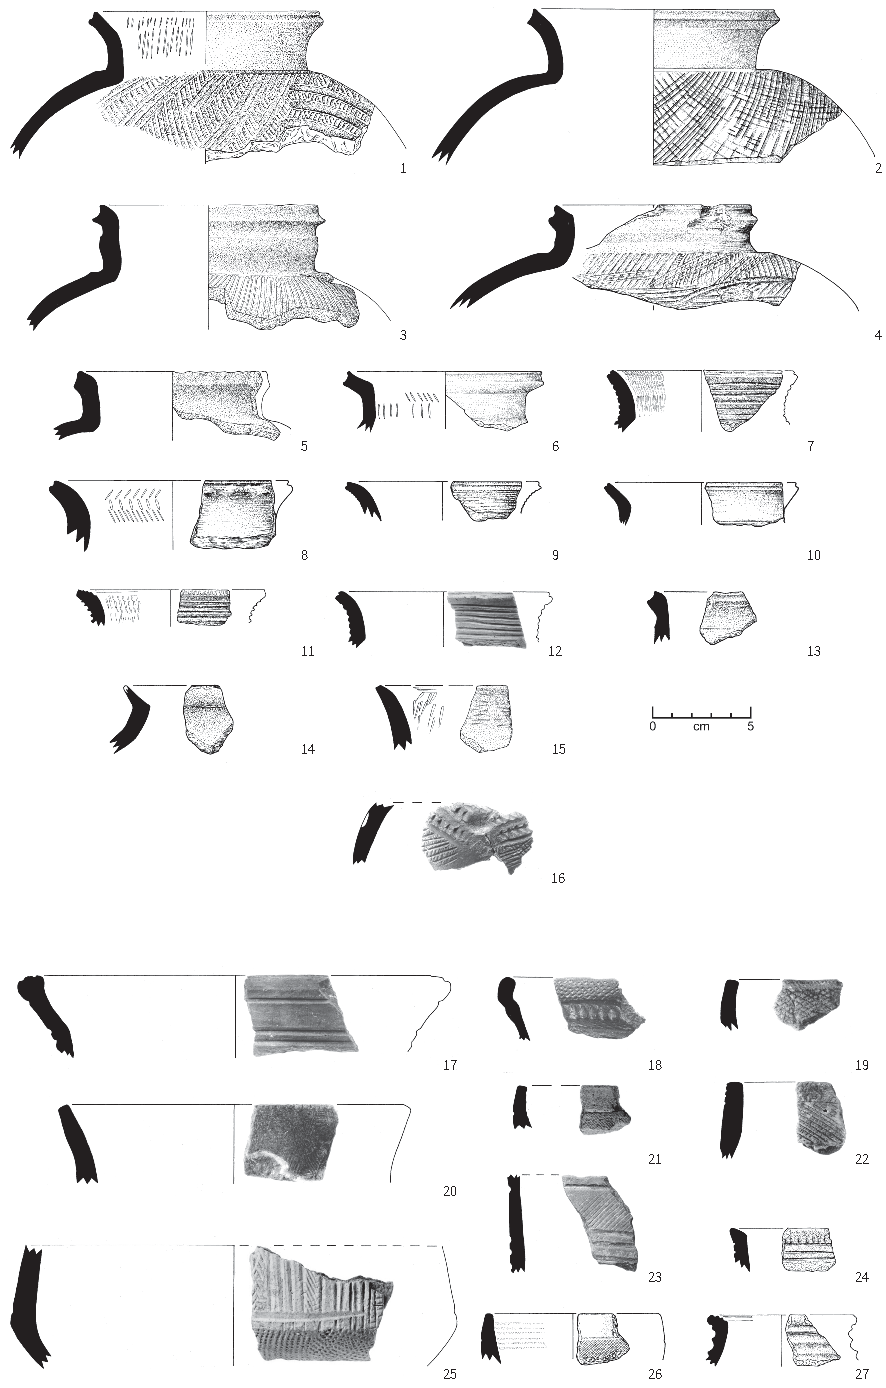
\includegraphics{plt/Taf48.pdf}
	\vspace{.75em}\caption{\mbox{Sangha}, Grabungsfunde \\ 1--19 PIK~87/1; 20--30 PIK~87/2.}
	\label{pl:48}
\end{pl}

\begin{pl}[H]
	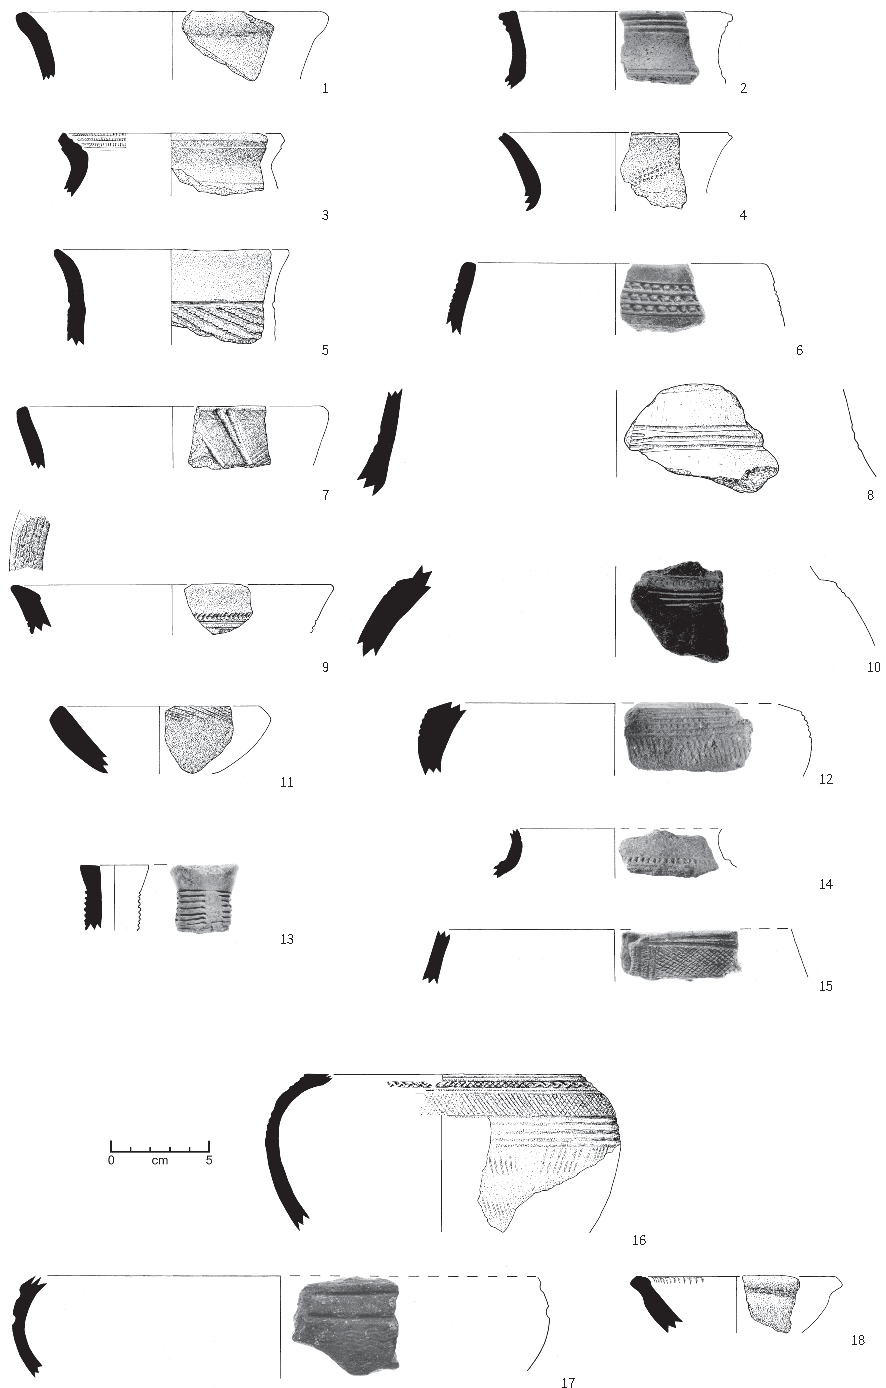
\includegraphics{plt/Taf49.pdf}
	\vspace{.75em}\caption{\mbox{Sangha}, Grabungsfunde \\ 1--16 PIK~87/2; 17--19 PIK~87/3.}
	\label{pl:49}
\end{pl}

\begin{pl}[H]
	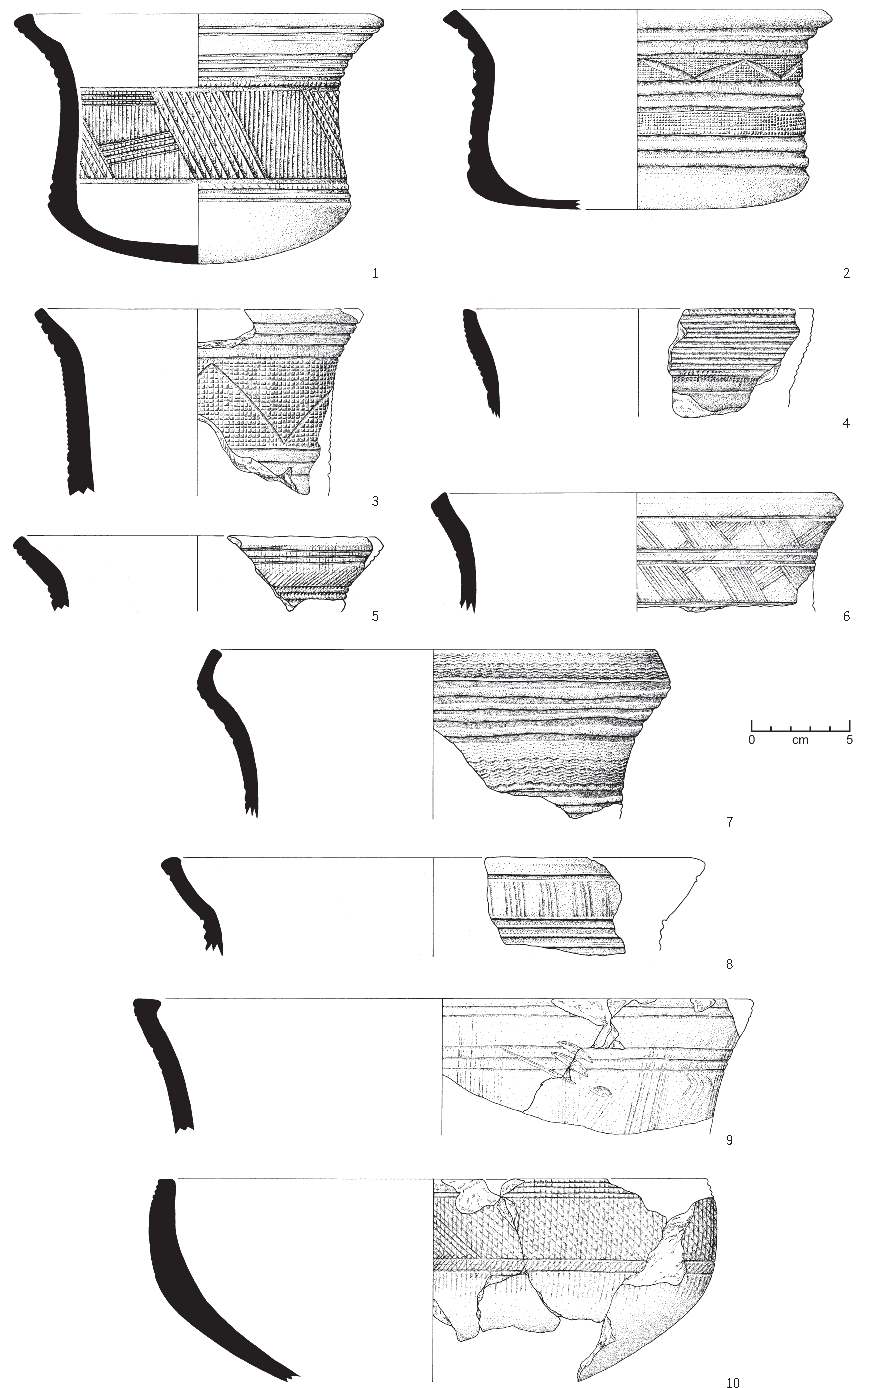
\includegraphics{plt/Taf50.pdf}
	\vspace{.75em}\caption{\mbox{Sangha}, Oberflächenfunde \\ 1--11 PIK~87/101.}
	\label{pl:50}
\end{pl}

\begin{pl}[H]
	\includegraphics{plt/Taf51.pdf}
	\vspace{.75em}\caption{\mbox{Sangha}, Oberflächenfunde \\ 1--13 PIK~87/101.}
	\label{pl:51}
\end{pl}

\begin{pl}[H]
	\includegraphics{plt/Taf52.pdf}
	\vspace{.75em}\caption{\mbox{Sangha}, Oberflächenfunde \\ 1--22 PIK~87/101.}
	\label{pl:52}
\end{pl}

\begin{pl}[H]
	\includegraphics{plt/Taf53.pdf}
	\vspace{.75em}\caption{\mbox{Sangha}, Oberflächenfunde \\ 1--15 PIK~87/101.}
	\label{pl:53}
\end{pl}

\begin{pl}[H]
	\includegraphics{plt/Taf54.pdf}
	\vspace{.75em}\caption{\mbox{Sangha}, Oberflächenfunde \\ 1--17 PIK~87/101.}
	\label{pl:54}
\end{pl}

\begin{pl}[H]
	\includegraphics{plt/Taf55.pdf}
	\vspace{.75em}\caption{\mbox{Sangha}, Oberflächenfunde \\ 1--17 PIK~87/101.}
	\label{pl:55}
\end{pl}

\begin{pl}[H]
	\includegraphics{plt/Taf56.pdf}
	\vspace{.75em}\caption{\mbox{Sangha}, Oberflächenfunde \\ 1--15 PIK~87/101; 16 PIK~87/102.}
	\label{pl:56}
\end{pl}

\begin{pl}[H]
	\includegraphics{plt/Taf57.pdf}
	\vspace{.75em}\caption{\mbox{Sangha}, Oberflächenfunde \\ 1--7 MLD~87/101; 8 MLD~87/102; 9--11 MLD~87/103; 12--27 MDB~87/101.}
	\label{pl:57}
\end{pl}

\begin{pl}[H]
	\includegraphics{plt/Taf58.pdf}
	\vspace{.75em}\caption{\mbox{Sangha}, Oberflächenfunde \\ 1--10 MDB~87/101; 11--25 IKM~87/101.}
	\label{pl:58}
\end{pl}

\begin{pl}[H]
	\includegraphics{plt/Taf59.pdf}
	\vspace{.75em}\caption{\mbox{Sangha}, Oberflächenfunde \\ 1--24 IKM~87/101; 25 MOS~87/101; 26--31 MAT~87/101.}
	\label{pl:59}
\end{pl}

\begin{pl}[H]
	\includegraphics{plt/Taf60.pdf}
	\vspace{.75em}\caption{\mbox{Sangha}, Oberflächenfunde \\ 1--18 MAT~87/101; 19--26 MAB~87/101.}
	\label{pl:60}
\end{pl}

\begin{pl}[H]
	\includegraphics{plt/Taf61.pdf}
	\vspace{.75em}\caption{\mbox{Sangha}, Oberflächenfunde \\ 1--15 KON~87/101; 16--17 LMS~87/101.}
	\label{pl:61}
\end{pl}

\begin{pl}[H]
	\includegraphics{plt/Taf62.pdf}
	\vspace{.75em}\caption{\mbox{Sangha}, Oberflächenfunde \\ 1 LMS~87/101; 2--5 MPB~87/101; 6--9 MPB~87/102; 10--14 MPB~87/101; 15--16 BDA~87/101.}
	\label{pl:62}
\end{pl}

\begin{pl}[H]
	\includegraphics{plt/Taf63.pdf}
	\vspace{.75em}\caption{\mbox{Sangha} \& \mbox{Ngoko}, Oberflächenfunde \\ 1--5 SAK~87/101; 6--20 PDM~87/101.}
	\label{pl:63}
\end{pl}

\begin{pl}[H]
	\includegraphics{plt/Taf64.pdf}
	\vspace{.75em}\caption{\mbox{Ngoko}, Oberflächenfunde \\ 1--15 PDM~87/101.}
	\label{pl:64}
\end{pl}

\begin{pl}[H]
	\includegraphics{plt/Taf65.pdf}
	\vspace{.75em}\caption{\mbox{Ngoko}, Oberflächenfunde \\ 1--10 PDM~87/101; 11--14 PDM~87/102.}
	\label{pl:65}
\end{pl}

\begin{pl}[H]
	\includegraphics{plt/Taf66.pdf}
	\vspace{.75em}\caption{\mbox{Ngoko}, Oberflächenfunde \\ 1--8 PDM~87/102; 9--15 MBJ~87/101; 16--20 NGA~87/101.}
	\label{pl:66}
\end{pl}

\begin{pl}[H]
	\includegraphics{plt/Taf67.pdf}
	\vspace{.75em}\caption{\mbox{Ngoko}, Oberflächenfunde \\ 1--23 NGA~87/101.}
	\label{pl:67}
\end{pl}

\begin{pl}[H]
	\includegraphics{plt/Taf68.pdf}
	\vspace{.75em}\caption{Likwala-aux-Herbes, Grabungs- \& Oberflächenfunde (1--3) \\ 1 NGA~87/101; 2--3 BYN~87/101; 4--5 BLK~87/1.}
	\label{pl:68}
\end{pl}

\begin{pl}[H]
	\includegraphics{plt/Taf69.pdf}
	\vspace{.75em}\caption{Likwala-aux-Herbes, Grabungs- \& Oberflächenfunde (5--8) \\ 1--4 BLK~87/1; 5--8 BLK~87/101.}
	\label{pl:69}
\end{pl}

\begin{pl}[H]
	\includegraphics{plt/Taf70.pdf}
	\vspace{.75em}\caption{Likwala-aux-Herbes, Oberflächenfunde \& Ankauf (5) \\ 1--4 BLK~87/101; 5 BLK~87/501.}
	\label{pl:70}
\end{pl}

\begin{pl}[H]
	\includegraphics{plt/Taf71.pdf}
	\vspace{.75em}\caption{Likwala-aux-Herbes, Oberflächenfunde \\ 1--5 BTW~87/101.}
	\label{pl:71}
\end{pl}

\begin{pl}[H]
	\includegraphics{plt/Taf72.pdf}
	\vspace{.75em}\caption{Likwala-aux-Herbes, Oberflächenfunde \\ 1 ILL~87/101; 2--9 MIS~87/101.}
	\label{pl:72}
\end{pl}

\begin{pl}[H]
	\includegraphics{plt/Taf73.pdf}
	\vspace{.75em}\caption{Likwala-aux-Herbes, Oberflächenfunde \\ 1 YUM~87/101; 2--11 YUM~87/102.}
	\label{pl:73}
\end{pl}

\begin{pl}[H]
	\includegraphics{plt/Taf74.pdf}
	\vspace{.75em}\caption{Likwala-aux-Herbes, Oberflächenfunde \\ 1--3 YUM~87/102; 4--10 YUM~87/103.}
	\label{pl:74}
\end{pl}

\begin{pl}[H]
	\includegraphics{plt/Taf75.pdf}
	\vspace{.75em}\caption{Likwala-aux-Herbes, Oberflächenfunde \\ 1--9 YUM~87/103.}
	\label{pl:75}
\end{pl}

\begin{pl}[H]
	\includegraphics{plt/Taf76.pdf}
	\vspace{.75em}\caption{Likwala-aux-Herbes, Oberflächenfunde \\ 1--11 LKW~87/186; 12--17 BJJ~87/101.}
	\label{pl:76}
\end{pl}

\begin{pl}[H]
	\includegraphics{plt/Taf77.pdf}
	\vspace{.75em}\caption{Likwala-aux-Herbes, Oberflächenfunde \\ 1--19 BJJ~87/101.}
	\label{pl:77}
\end{pl}

\begin{pl}[H]
	\includegraphics{plt/Taf78.pdf}
	\vspace{.75em}\caption{Likwala-aux-Herbes, Oberflächenfunde \\ 1--17 BJJ~87/101.}
	\label{pl:78}
\end{pl}

\begin{pl}[H]
	\includegraphics{plt/Taf79.pdf}
	\vspace{.75em}\caption{Likwala-aux-Herbes, Oberflächenfunde \\ 1--3 BJJ~87/101; 4 BKA~87/101; 5--10 MSN~87/101.}
	\label{pl:79}
\end{pl}

\begin{pl}[H]
	\includegraphics{plt/Taf80.pdf}
	\vspace{.75em}\caption{Likwala-aux-Herbes, Oberflächenfunde \\ 1--9 MSN~87/101.}
	\label{pl:80}
\end{pl}

\begin{pl}[H]
	\includegraphics{plt/Taf81.pdf}
	\vspace{.75em}\caption{Likwala-aux-Herbes, Oberflächenfunde \\ 1--18 EBA~87/101.}
	\label{pl:81}
\end{pl}

\begin{pl}[H]
	\includegraphics{plt/Taf82.pdf}
	\vspace{.75em}\caption{Likwala-aux-Herbes, Oberflächenfunde \\ 1--12 EBA~87/101.}
	\label{pl:82}
\end{pl}

\begin{pl}[H]
	\includegraphics{plt/Taf83.pdf}
	\vspace{.75em}\caption{Likwala-aux-Herbes, Oberflächenfunde \\ 1--15 EBA~87/101.}
	\label{pl:83}
\end{pl}

\begin{pl}[H]
	\includegraphics{plt/Taf84.pdf}
	\vspace{.75em}\caption{Likwala-aux-Herbes, Oberflächenfunde \\ 1 BWA~87/102; 2--9 MSG~87/101.}
	\label{pl:84}
\end{pl}

\begin{pl}[H]
	\includegraphics{plt/Taf85.pdf}
	\vspace{.75em}\caption{Likwala-aux-Herbes, Oberflächenfunde \\ 1--3 MSG~87/101; 4--8 MSG~87/102.}
	\label{pl:85}
\end{pl}

\begin{pl}[H]
	\includegraphics{plt/Taf86.pdf}
	\vspace{.75em}\caption{Likwala-aux-Herbes, Oberflächenfunde \\ 1--2 MSG~87/102; 3--6 LKN~87/101.}
	\label{pl:86}
\end{pl}

\begin{pl}[H]
	\includegraphics{plt/Taf87.pdf}
	\vspace{.75em}\caption{Likwala-aux-Herbes, Oberflächenfunde \\ 1--2 LKN~87/101; 3 LKW~87/401; 4--9 EPE~87/101.}
	\label{pl:87}
\end{pl}

\begin{pl}[H]
	\includegraphics{plt/Taf88.pdf}
	\vspace{.75em}\caption{Likwala-aux-Herbes, Grabungs- \& Oberflächenfunde (1--5) \\ 1--5 EPE~87/101; 6--11 MUN~87/1.}
	\label{pl:88}
\end{pl}

\begin{pl}[H]
	\includegraphics{plt/Taf89.pdf}
	\vspace{.75em}\caption{Likwala-aux-Herbes, Grabungsfunde \\ 1--8 MUN 87/1.}
	\label{pl:89}
\end{pl}

\begin{pl}[H]
	\includegraphics{plt/Taf90.pdf}
	\vspace{.75em}\caption{Likwala-aux-Herbes, Grabungsfunde \\ 1--2 MUN 87/1.}
	\label{pl:90}
\end{pl}

\begin{pl}[H]
	\includegraphics{plt/Taf91.pdf}
	\vspace{.75em}\caption{Likwala-aux-Herbes, Grabungsfunde \\ 1--8 MUN~87/2-1-1.}
	\label{pl:91}
\end{pl}

\begin{pl}[H]
	\includegraphics{plt/Taf92.pdf}
	\vspace{.75em}\caption{Likwala-aux-Herbes, Grabungsfunde \\ 1--9 MUN~87/2-1-3.}
	\label{pl:92}
\end{pl}

\begin{pl}[H]
	\includegraphics{plt/Taf93.pdf}
	\vspace{.75em}\caption{Likwala-aux-Herbes, Grabungsfunde \\ 1--8 MUN~87/2-1-3.}
	\label{pl:93}
\end{pl}

\begin{pl}[H]
	\includegraphics{plt/Taf94.pdf}
	\vspace{.75em}\caption{Likwala-aux-Herbes, Grabungsfunde \\ 1--3 MUN~87/3; 4--5 MUN~87/101; 6--9 ITN~87/101.}
	\label{pl:94}
\end{pl}

\begin{pl}[H]
	\includegraphics{plt/Taf95.pdf}
	\vspace{.75em}\caption{Likwala-aux-Herbes, Oberflächenfunde \\ 1--5 ITN~87/101.}
	\label{pl:95}
\end{pl}

\begin{pl}[H]
	\includegraphics{plt/Taf96.pdf}
	\vspace{.75em}\caption{Likwala-aux-Herbes, Oberflächenfunde \\ 1--3 ITN~87/101.}
	\label{pl:96}
\end{pl}

\begin{pl}[H]
	\includegraphics{plt/Taf97.pdf}
	\vspace{.75em}\caption{Likwala-aux-Herbes, Oberflächenfunde \\ 1--6 ITN~87/101; 7--9 EPE~87/101.}
	\label{pl:97}
\end{pl}

\begin{pl}[H]
	\includegraphics{plt/Taf98.pdf}
	\vspace{.75em}\caption{\mbox{Sangha}, Oberflächenfunde \\ OUE~87/101: 1 Faustkeil; 2--6 Abschläge (Fotos: D.~Seidensticker).}
	\label{pl:98}
\end{pl}